\documentclass{article}
\usepackage{graphicx} % Required for inserting images
\usepackage{hyperref}
\usepackage{tikz}
\usepackage{amsmath}
\usepackage{amssymb}
\usepackage{algorithm}
\usepackage{algpseudocode}
\algrenewcommand{\algorithmiccomment}[1]{\hfill\textcolor{black!50}{\footnotesize\itshape$\triangleright$\,#1}}
\usetikzlibrary{arrows.meta,calc,decorations.pathmorphing,decorations.pathreplacing}
\usepackage[scr=boondox]{mathalpha}
\usepackage[font=footnotesize,margin=-2.5em,skip=7pt]{caption}
\newcommand{\logits}{\mathrm{logits}}
\newcommand{\smax}{\mathrm{Softmax}}
\newcommand{\norm}{\mathrm{norm}}
\newcommand{\jlens}{\mathscr{L}}
\newcommand{\jspace}{\mathscr{S}}
\newcommand{\dispersion}{\mathscr{D}}
\newcommand{\alignment}{\mathscr{A}}
\newcommand{\dmodel}{d_{\text{model}}}
\DeclareMathOperator*{\argmin}{arg\,min}
\DeclareMathOperator*{\argmax}{arg\,max}

\tikzset{
  jblock/.style={draw,thick,fill=gray!12,minimum width=15mm,minimum height=7mm,font=\small},
  jslab/.style={draw,thick,fill=gray!10,minimum width=82mm,minimum height=8mm},
  jmini/.style={draw,thick,fill=gray!12,minimum width=9mm,minimum height=5mm,font=\scriptsize},
  jattn/.style={-{Stealth[length=2mm]},thin,gray!55},
  jattnS/.style={-{Stealth[length=1.6mm]},thin,gray!55},
  jresid/.style={line width=1.1pt},
  jlab/.style={font=\small},
  jlabS/.style={font=\scriptsize},
  cordJ/.style={line width=1pt,gray!55},
  jband/.style={draw,thick,fill=gray!14,minimum width=22mm,minimum height=5mm,font=\scriptsize},
}

\colorlet{jyel}{yellow!85!orange!90!black}
\colorlet{jblu}{blue!65}
\colorlet{jred}{red!75}
\colorlet{jgrn}{green!55!black}
\colorlet{jdn}{red!65!black}
\colorlet{jvio}{violet!85!black}
\colorlet{jtea}{teal!65!black}
\colorlet{jorg}{orange!90!black}
% --- Figure 2 content-mixing (pigment) colors: yellow+blue=green, +red=brown ---
\colorlet{jmixYB}{green!65!black}
\colorlet{jmixBR}{purple!80!black}
\colorlet{jmixYBR}{brown!70!black}
% --- J-space figure colors (A: RGB basis; B: red->green band + stranded blue) ---
\definecolor{hrust}{RGB}{184,87,31}\definecolor{hteal}{RGB}{31,133,143}\definecolor{hplum}{RGB}{133,56,148}
\definecolor{primR}{RGB}{224,38,38}\definecolor{primG}{RGB}{30,182,60}\definecolor{primB}{RGB}{44,72,224}
\definecolor{Ddr}{RGB}{230,20,20}\definecolor{Ddo}{RGB}{255,128,0}\definecolor{Ddc}{RGB}{128,220,0}\definecolor{Ddg}{RGB}{0,200,0}
\definecolor{BhT}{RGB}{217,217,140}\definecolor{BrA}{RGB}{0,87,140}\definecolor{BrB}{RGB}{0,0,140}
% --- frequency figure colors ---
\definecolor{fgrab}{RGB}{42,125,42}\definecolor{frem}{RGB}{192,32,32}

\newcommand{\jlogits}[2]{% #1 = x center, #2 = y of baseline
  \draw (#1-0.62,#2+0.85) -| (#1-0.74,#2-0.35) -- (#1-0.62,#2-0.35);
  \draw (#1+0.62,#2+0.85) -| (#1+0.74,#2-0.35) -- (#1+0.62,#2-0.35);
  \draw[gray!40,thin] (#1-0.55,#2) -- (#1+0.55,#2);
  \foreach \i/\v in {0/0.35,1/-0.15,2/0.7,3/0.2,4/-0.3,5/0.55,6/0.1}{
    \draw[line width=0.9pt] (#1-0.45+\i*0.15,#2) -- ++(0,\v);}}

\newcommand{\jglyph}[3]{% #1 = y center (x=0 local), #2 = J-part color, #3 = remainder color
  \draw (-0.5,#1+0.45) -| (-0.62,#1-0.45) -- (-0.5,#1-0.45);
  \draw (0.5,#1+0.45) -| (0.62,#1-0.45) -- (0.5,#1-0.45);
  \draw[#2,line width=2.8pt] (0,#1+0.38) -- (0,#1+0.2);
  \draw[#3,line width=2.8pt] (0,#1+0.08) -- (0,#1-0.38);}

\newcommand{\jbarframe}[2]{% #1 = x center, #2 = y of axis
  \draw (#1-0.62,#2+1.15) -| (#1-0.74,#2-0.5) -- (#1-0.62,#2-0.5);
  \draw (#1+0.62,#2+1.15) -| (#1+0.74,#2-0.5) -- (#1+0.62,#2-0.5);
  \draw[gray!40,thin] (#1-0.55,#2) -- (#1+0.55,#2);}

\title{J-Vision}
\author{Ben Meyers}
\date{July 2026}

\begin{document}

\maketitle

\section{Through the Jacobian Lens}

Anthropic's recent \href{https://transformer-circuits.pub/2026/workspace/index.html}{paper} introduce the \textbf{J-lens} and the \textbf{J-space}, a new causal lensing approach to interpret the cognition of Large Language Models (LLMs). 

The contract of deep learning is (1) legible \textit{ends} (input/output) and (2) \textit{end-to-end} differentiability. By configuring our desired behavior (such as predicting text from text) as a program that type-checks the above contract, we invite backpropagation to causally map the network and iteratively realize our goals through it. Training is a series of instantaneous lenses (how can \textit{this error} be related to \textit{these current parameters} and reduced in their terms?), accumulated into expectations (which parameters, in general, have the most bearing on \textit{average} error and how should we change them?), which are then committed as parameter updates. Inference is a local instant---we \textit{want} inference to be local and specific---but with the \textbf{J-lens} we construct an \textit{expected} lens on how those instants behave in general. We trained with expectation, so now let's reverse-engineer with it. Figure~\ref{fig:four-square} shows a matrix of four kinds of lenses endowed by the contract and used in training and interpretability. 

%% The four derivative objects. Reference as Figure~\ref{fig:four-square}.
\begin{figure}[htbp]
\centering
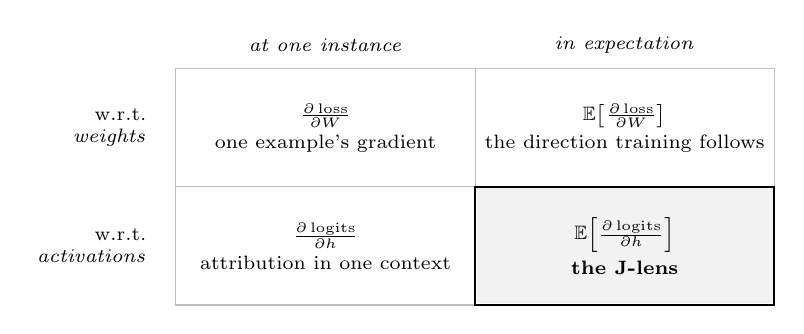
\begin{tikzpicture}[cell/.style={font=\scriptsize,align=center}]
\draw[gray!50] (0,0) rectangle (7.6,3.0);
\draw[gray!50] (3.8,0) -- (3.8,3.0);
\draw[gray!50] (0,1.5) -- (7.6,1.5);
\node[cell] at (1.9,3.3)  {\emph{at one instance}};
\node[cell] at (5.7,3.3)  {\emph{in expectation}};
\node[cell,anchor=east,align=right] at (-0.25,2.25) {w.r.t.\\ \emph{weights}};
\node[cell,anchor=east,align=right] at (-0.25,0.75) {w.r.t.\\ \emph{activations}};
\node[cell] at (1.9,2.25) {$\frac{\partial\,\mathrm{loss}}{\partial W}$\\[2pt] one example's gradient};
\node[cell] at (5.7,2.25) {$\mathbb{E}\!\left[\frac{\partial\,\mathrm{loss}}{\partial W}\right]$\\[2pt] the direction training follows};
\node[cell] at (1.9,0.75) {$\frac{\partial\,\logits}{\partial h}$\\[2pt] attribution in one context};
\fill[gray!10] (3.82,0.02) rectangle (7.58,1.48);
\node[cell] at (5.7,0.75) {$\mathbb{E}\!\left[\frac{\partial\,\logits}{\partial h}\right]$\\[2pt] \textbf{the J-lens}};
\draw[thick] (3.8,0) rectangle (7.6,1.5);
\end{tikzpicture}
\caption{Four derivative objects from the same contract. The top row has always steered \emph{training}; the bottom-left explains single predictions after the fact. The fourth square---activation Jacobians taken \emph{in expectation}---is the new instrument.}
\label{fig:four-square}
\end{figure}


The \textbf{J-lens} is an expected derivative of \textit{logits}---scores given by the model to the tokens at its disposal for sampling next---with respect to \textit{activations}---the forward-propagating internal state of the model. It is a matrix, where each \(v\)-th row represents the logit index for token \(v\) in the vocabulary, and each \(d\)-th column of row \(v\) denotes the influence of activation dimension \(d\) on that \(v\)-th token. It doesn't give us static data about what the activations \textit{stand for}, but instead where they \textit{point}. This matrix can then attribute disposition---in terms of \textit{tokens}, which stand for \textit{concepts}---to the heretofore inscrutable latent space of the model. 

It is important to impress that the \textbf{J-lens} doesn't just \textit{correlate} internal activations with external verbalization potentials. It does not offer a merely statistical picture of interpretability, where statements can be made to the effect of: ``this circuit of neurons always seems to fire when the model discusses dogs, so therefore this circuit may encode something about dogs.'' These networks (when trained) are entirely deterministic and static; these Jacobians speak only the language of analytically-derived \textit{cause}. They allow us to say: ``this bundle of activated neurons reflects that the model is disposed to mention dogs; if we amplify these currently-activated neurons, the model \textit{will} mention dogs more.''

Further, once the directions in the model's activation space are inflected conceptually, we can do better than just \textit{identify} disposition implied by state. We can tap the tools from the abstract formalism of linear algebra to work---steer, perturb and observe, illustratively decompose---in a now-interpretable space with economy. Cue the \textbf{J-space}. The \textbf{J-lens} gives us white light---true, but over-saturated and noisy. The \textbf{J-space} is a prism fit on this light, in the form of a linear decomposition. Through it, we only keep those \textbf{J-lens} directions that hold the disproportionate weight of that disposition.\footnote{If we can expect to see anything like cognition and thoughts inside a language model, we have to hope that they can be put in the reduced terms of a few dozen---not dozens of thousands---of concepts.} The prism proves more than pretty; the \textbf{J-space} has been shown (in diverse though duly limited experiments, detailed in \S\ref{jvizllm}) as a privileged seat of interventional opportunity in LLMs. 


This document will explain the definitions and techniques employed to compute the \textbf{J-lens} and the \textbf{J-space} and will seek to elucidate how fruitful our chosen formulation for deep learning---\textit{differentiable vector spaces}---is and can continue to be. 

\section{Transformer Architecture: Positions, Layers, Logits, the Residual Stream, and Normalization}




%% A (v2.2): one column of weights, S residual streams; Anthropic index convention
\begin{figure}[htbp]
\centering
\resizebox{0.95\textwidth}{!}{%
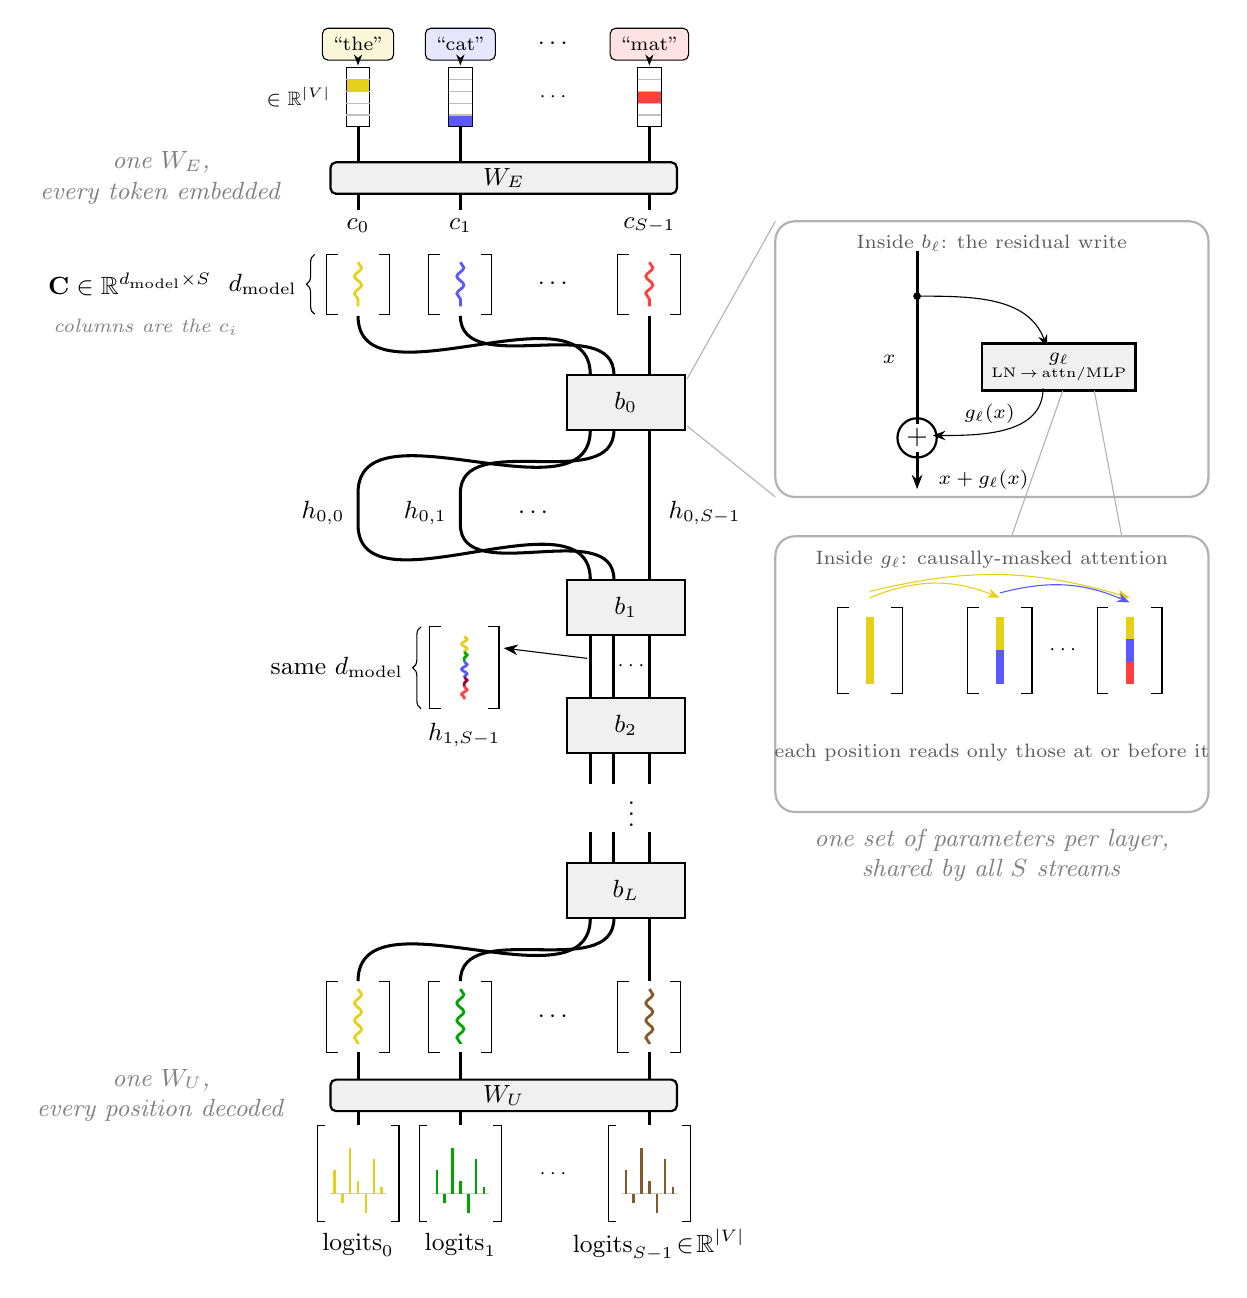
\begin{tikzpicture}
% ---- top: C matrix framing + input context vectors c_0 ... c_S
\node[jlab,align=center] at (-6.3,0.0)
      {$\mathbf{C} \in \mathbb{R}^{\dmodel \times S}$};
% \draw[-{Stealth[length=1.8mm]},gray] (-5.35,-0.15) -- (-4.35,-0.05);
\node[jlabS,gray] at (-6.1,-0.55) {\emph{columns are the $c_i$}};
\node[jlab] at (-3.4,0.75) {$c_0$}; \node[jlab] at (-2.1,0.75) {$c_1$};
\node[jlab] at (-0.9,0.0) {$\cdots$}; \node[jlab] at (0.3,0.75) {$c_{S-1}$};
\foreach \X/\tc in {-3.4/jyel,-2.1/jblu,0.3/jred}{
  \draw (\X-0.26,0.38) -| (\X-0.40,-0.38) -- (\X-0.26,-0.38);
  \draw (\X+0.26,0.38) -| (\X+0.40,-0.38) -- (\X+0.26,-0.38);
  \draw[\tc,line width=1pt,decorate,decoration={snake,amplitude=.45mm,segment length=2.2mm}]
        (\X,0.28) -- (\X,-0.28);}
\draw[decorate,decoration={brace,mirror,amplitude=3pt}] (-3.95,0.38) -- (-3.95,-0.38)
      node[midway,left=3pt,jlab]{$\dmodel$};
% ---- input embedding: text -> one-hots -> one shared W_E -> the c_i (mirror of the unembed below)
\node[draw,rounded corners=2pt,fill=jyel!15,font=\scriptsize] at (-3.4,3.05) {``the''};
\node[draw,rounded corners=2pt,fill=jblu!15,font=\scriptsize] at (-2.1,3.05) {``cat''};
\node[jlab] at (-0.9,3.05) {$\cdots$};
\node[draw,rounded corners=2pt,fill=jred!15,font=\scriptsize] at (0.3,3.05) {``mat''};
\foreach \X/\vc/\fy in {-3.4/jyel/2.60,-2.1/jblu/2.15,0.3/jred/2.45}{
  \fill[\vc] (\X-0.15,\fy) rectangle (\X+0.15,\fy-0.15);
  \draw (\X-0.15,2.75) rectangle (\X+0.15,2.0);
  \foreach \yy in {2.60,2.45,2.30,2.15}{\draw[gray!50] (\X-0.15,\yy) -- (\X+0.15,\yy);}}
\node[jlabS] at (-0.9,2.375) {$\cdots$};
\node[jlabS,left] at (-3.62,2.375) {$\in\mathbb{R}^{|V|}$};
\draw[thick,fill=gray!12,rounded corners=2pt] (-3.75,1.15) rectangle (0.65,1.55);
\node[font=\small] at (-1.55,1.35) {$W_E$};
\foreach \X in {-3.4,-2.1,0.3}{
  \draw[-{Stealth[length=1.4mm]}] (\X,2.88) -- (\X,2.78);
  \draw[jresid] (\X,2.0) -- (\X,1.55);
  \draw[jresid] (\X,1.15) -- (\X,0.95);}
\node[jlab,gray,align=center] at (-5.9,1.35) {\emph{one $W_E$,}\\ \emph{every token embedded}};
% ---- the single stack of blocks (ONE set of weights per layer)
\node[jblock] (b0) at (0,-1.5) {$b_0$};
\node[jblock] (b1) at (0,-4.1) {$b_1$};
\node[jblock] (b2) at (0,-5.6) {$b_2$};
\node[jblock] (bL) at (0,-7.7) {$b_L$};
% ---- streams into b_0
\draw[jresid] (-3.4,-0.40) to[out=-90,in=90] (-0.45,-1.15);
\draw[jresid] (-2.1,-0.40) to[out=-90,in=90] (-0.15,-1.15);
\draw[jresid] (0.3,-0.40) -- (0.3,-1.15);
% ---- ONE big nested cutaway of b_0: (1) residual write (vertical cord, g_ell branches to the side); (2) g_ell opens DOWN into attention.
% connector: b_0 -> Window 1
\draw[gray!60,thin] (0.78,-1.2) -- (1.9,0.8);
\draw[gray!60,thin] (0.78,-1.8) -- (1.9,-2.7);
% ===== Window 1: the residual write =====
\draw[rounded corners=7pt,thick,gray!60] (1.9,0.8) rectangle (7.4,-2.7);
\node[jlabS,gray!70!black] at (4.65,0.52) {Inside $b_\ell$: the residual write};
% the residual cord: split near the top, sum lower down, output continues
\draw[jresid] (3.7,0.42) -- (3.7,-0.15);
\fill (3.7,-0.15) circle (1.4pt);
\draw[jresid] (3.7,-0.15) -- (3.7,-1.77);
\node[jlabS,left] at (3.55,-0.95) {$x$};
\node[draw,circle,inner sep=1.4pt,thick] at (3.7,-1.95) {$+$};
\draw[jresid,-{Stealth[length=1.8mm]}] (3.7,-2.13) -- (3.7,-2.6);
\node[jlabS,right] at (3.85,-2.48) {$x + g_\ell(x)$};
% branch off to the side, through g_ell, back into the sum
\draw[thin,-{Stealth[length=1.6mm]}] (3.7,-0.15) to[out=0,in=110] (5.35,-0.8);
\node[draw,thick,fill=gray!12,font=\scriptsize,align=center] at (5.5,-1.05) {$g_\ell$\\[-2pt] {\tiny LN\,$\to$\,attn/MLP}};
\draw[thin,-{Stealth[length=1.6mm]}] (5.3,-1.32) to[out=-90,in=0] (3.9,-1.92);
\node[jlabS] at (4.62,-1.64) {$g_\ell(x)$};
% connector: the g_ell box opens straight DOWN into Window 2
\draw[gray!60,thin] (5.55,-1.35) -- (4.9,-3.2);
\draw[gray!60,thin] (5.95,-1.35) -- (6.3,-3.2);
% ===== Window 2: g_ell opened = causally-masked attention (roomy, below) =====
\draw[rounded corners=7pt,thick,gray!60] (1.9,-3.2) rectangle (7.4,-6.7);
\node[jlabS,gray!70!black] at (4.65,-3.5) {Inside $g_\ell$: causally-masked attention};
\foreach \X in {3.1,4.75,6.4}{
  \draw (\X-0.27,-4.1) -| (\X-0.41,-5.2) -- (\X-0.27,-5.2);
  \draw (\X+0.27,-4.1) -| (\X+0.41,-5.2) -- (\X+0.27,-5.2);}
\draw[jyel,line width=3pt] (3.1,-4.22) -- (3.1,-5.08);
\draw[jyel,line width=3pt] (4.75,-4.22) -- (4.75,-4.65);
\draw[jblu,line width=3pt] (4.75,-4.65) -- (4.75,-5.08);
\draw[jyel,line width=3pt] (6.4,-4.22) -- (6.4,-4.51);
\draw[jblu,line width=3pt] (6.4,-4.51) -- (6.4,-4.79);
\draw[jred,line width=3pt] (6.4,-4.79) -- (6.4,-5.08);
\node[jlabS] at (5.575,-4.65) {$\cdots$};
\draw[jattnS,jyel] (3.1,-3.98) to[bend left=22] (4.75,-3.98);
\draw[jattnS,jyel] (3.1,-3.9) to[bend left=15] (6.4,-3.98);
\draw[jattnS,jblu] (4.75,-3.92) to[bend left=19] (6.4,-4.04);
\node[jlabS,gray!70!black,align=center] at (4.65,-5.95) {each position reads only those at or before it};
% ---- after b_0: pull the streams out and NAME them (they are the positions)
\draw[jresid] (-0.45,-1.85) to[out=-90,in=90] (-3.4,-2.65) -- (-3.4,-3.05)
              to[out=-90,in=90] (-0.45,-3.75);
\draw[jresid] (-0.15,-1.85) to[out=-90,in=90] (-2.1,-2.65) -- (-2.1,-3.05)
              to[out=-90,in=90] (-0.15,-3.75);
\draw[jresid] (0.3,-1.85) -- (0.3,-3.75);
\node[jlab,left]  at (-3.45,-2.9) {$h_{0,0}$};
\node[jlab,left]  at (-2.15,-2.9) {$h_{0,1}$};
\node[jlab]       at (-1.15,-2.9) {$\cdots$};
\node[jlab,right] at (0.42,-2.9)  {$h_{0,S-1}$};
% ---- after b_1: tap with full d_model vector (shape preserved)
\draw[jresid] (-0.45,-4.45) -- (-0.45,-5.25);
\draw[jresid] (-0.15,-4.45) -- (-0.15,-5.25);
\draw[jresid] (0.3,-4.45) -- (0.3,-5.25);
\node[jlabS] at (0.090,-4.85) {$\cdots$};
\draw[-{Stealth[length=1.8mm]}] (-0.49,-4.75) -- (-1.55,-4.62);
\draw (-2.35,-4.35) -| (-2.49,-5.39) -- (-2.35,-5.39);
\draw (-1.75,-4.35) -| (-1.61,-5.39) -- (-1.75,-5.39);
% h_{1,S-1}: the three content colors, one layer in --- beginning to mix (soft-blended borders)
\draw[jyel,line width=1pt,decorate,decoration={snake,amplitude=.35mm,segment length=1.2mm}] (-2.05,-4.47) -- (-2.05,-4.67);
\draw[jmixYB,line width=1pt,decorate,decoration={snake,amplitude=.35mm,segment length=1.2mm}] (-2.05,-4.67) -- (-2.05,-4.79);
\draw[jblu,line width=1pt,decorate,decoration={snake,amplitude=.35mm,segment length=1.2mm}] (-2.05,-4.79) -- (-2.05,-4.99);
\draw[jmixBR,line width=1pt,decorate,decoration={snake,amplitude=.35mm,segment length=1.2mm}] (-2.05,-4.99) -- (-2.05,-5.11);
\draw[jred,line width=1pt,decorate,decoration={snake,amplitude=.35mm,segment length=1.2mm}] (-2.05,-5.11) -- (-2.05,-5.27);
\draw[decorate,decoration={brace,mirror,amplitude=3pt}] (-2.60,-4.35) -- (-2.60,-5.39)
      node[midway,left=3pt,jlab]{same $\dmodel$};
\node[jlab] at (-2.05,-5.72) {$h_{1,S-1}$};
% ---- bundled cords downward
\draw[jresid] (-0.45,-5.95) -- (-0.45,-6.35);
\draw[jresid] (-0.15,-5.95) -- (-0.15,-6.35);
\draw[jresid] (0.3,-5.95) -- (0.3,-6.35);
\node[jlab] at (0.072,-6.62) {$\vdots$};
\draw[jresid] (-0.45,-6.95) -- (-0.45,-7.35);
\draw[jresid] (-0.15,-6.95) -- (-0.15,-7.35);
\draw[jresid] (0.3,-6.95) -- (0.3,-7.35);
% ---- the point, stated on-figure
\node[jlab,gray,align=center] at (4.65,-7.25)
      {\emph{one set of parameters per layer,}\\ \emph{shared by all $S$ streams}};
% (the residual write is now the FIRST nested window off b_0, above; g_ell there opens into attention)
% ---- bottom: fan back out; unembed only the final stream
\draw[jresid] (-0.45,-8.05) to[out=-90,in=90] (-3.4,-8.85);
\draw[jresid] (-0.15,-8.05) to[out=-90,in=90] (-2.1,-8.85);
\draw[jresid] (0.3,-8.05) -- (0.3,-8.85);
% final latents, fully mixed: h_{L,0} pure yellow, h_{L,1} green (Y+B), h_{L,S-1} brown (Y+B+R)
\foreach \X/\vc in {-3.4/jyel,-2.1/jmixYB,0.3/jmixYBR}{
  \draw (\X-0.26,-8.85) -| (\X-0.40,-9.75) -- (\X-0.26,-9.75);
  \draw (\X+0.26,-8.85) -| (\X+0.40,-9.75) -- (\X+0.26,-9.75);
  \draw[\vc,line width=1pt,decorate,decoration={snake,amplitude=.45mm,segment length=2.2mm}]
        (\X,-8.95) -- (\X,-9.65);}
\node[jlab] at (-0.9,-9.3) {$\cdots$};
% ---- unembed EVERY final stream through one shared W_U (mirror of W_E at top)
\draw[jresid] (-3.4,-9.75) -- (-3.4,-10.1);
\draw[jresid] (-2.1,-9.75) -- (-2.1,-10.1);
\draw[jresid] (0.3,-9.75) -- (0.3,-10.1);
\draw[thick,fill=gray!12,rounded corners=2pt] (-3.75,-10.5) rectangle (0.65,-10.1);
\node[font=\small] at (-1.55,-10.3) {$W_U$};
\draw[jresid] (-3.4,-10.5) -- (-3.4,-10.68);
\draw[jresid] (-2.1,-10.5) -- (-2.1,-10.68);
\draw[jresid] (0.3,-10.5) -- (0.3,-10.68);
\foreach \X/\vc in {-3.4/jyel,-2.1/jmixYB,0.3/jmixYBR}{
  \draw (\X-0.42,-10.68) -| (\X-0.52,-11.9) -- (\X-0.42,-11.9);
  \draw (\X+0.42,-10.68) -| (\X+0.52,-11.9) -- (\X+0.42,-11.9);
  \draw[gray!40,thin] (\X-0.36,-11.55) -- (\X+0.36,-11.55);
  \foreach \i/\v in {0/0.30,1/-0.12,2/0.58,3/0.16,4/-0.24,5/0.44,6/0.09}{
    \draw[\vc,line width=0.9pt] (\X-0.3+\i*0.1,-11.55) -- ++(0,\v);}}
\node[jlabS] at (-0.9,-11.3) {$\cdots$};
\node[jlab] at (-3.4,-12.2) {$\logits_0$};
\node[jlab] at (-2.1,-12.2) {$\logits_1$};
\node[jlab] at (0.42,-12.2) {$\logits_{S-1}\!\in\!\mathbb{R}^{|V|}$};
\node[jlab,gray,align=center] at (-5.9,-10.3) {\emph{one $W_U$,}\\ \emph{every position decoded}};
\end{tikzpicture}}
% CAPTION STUB (Ben to expand): the old long caption was trimmed at Ben's request.
\caption{The transformer as one stack of blocks $b_\ell$ and $S$ residual streams: tokens enter as text, become one-hots, and are mapped by a single shared $W_E$ into the columns $c_i$ of $\mathbf{C}$ (top); the blocks carry and mix these residual states through depth; and every final latent is decoded by a single shared $W_U$ into its logits (bottom). Colors trace content---each token enters in its own hue, attention \emph{moves} it across positions, and depth \emph{mixes} the bands into the final blended states.}
\label{fig:transformer-grid}
\end{figure}



To appreciate the \textbf{J-lens} and the \textbf{J-space}, a review of some principal components of the \textbf{Transformer} neural network architecture (that which carries out most modern LLMs) is in order. The key elements we'll discuss are:

\begin{enumerate}
    \item The manner in which token \textbf{Position} is represented and handled in the transformer's computation
    \item The way computation propagates forward through the \textbf{Layers} of the network
    \item The key output of the network which represents its prediction for best choice of \textit{next} token, the non-normalized vector of \textbf{Logits}
    \item The cord which carries \textit{state} through the layers of the model, the \textbf{Residual Stream}
    \item \textbf{Normalization} as a mechanism of abstraction in spatial representation
\end{enumerate}

At a high level, the transformer takes as input a context matrix, \(\mathbf{C}\), where each column, \(c_i\), represents a token of input as a vector.\footnote{This explanation of transformers ignores tokenization, one-hot representation, and embeddings and jumps right to contexts as being already embedded. Figure~\ref{fig:transformer-grid} hints at the tokenization and embedding stages, but they are less pertinent to the \textbf{J-lens} and \textbf{J-space}.} The transformer admits any sequence length, \(S\), meaning \(\mathbf{C}\)'s column count is \textit{free}. The dimension of each \(c_i\), though, is fixed model-wide at \(\dmodel\). The network's weights contract against \(\dmodel\), so \(S\) naturally carries forward seamlessly through each layer.

Strictly speaking, the transformer computes \(S\) final activation vectors, \(h_{L, t}\), for all \(t < S\).\footnote{A note on subscripts, used throughout: the first indexes the \textit{layer boundary}---\(h_{\ell, t}\) is the residual state at position \(i\) just after block \(b_\ell\), with \(L\) reserved for the final layer---and the second indexes the \textit{position}. At various points in the document, either subscript will be omitted when it doesn't detract from what is being explained; if there is only one subscript, it corresponds to \textit{layer}.} Though during training, it is performed on all final activations, once the model is trained and ready to be used for autoregressive \textit{generation}, only the final activation \(h_{L, S-1}\) is decoded via an \textit{un}embedding matrix, \(\mathbf{W_U} \in \mathbb{R}^{|V| \times \dmodel}\), where \(V\) is the token vocabulary and \(|V|\) its size. This decoding produces a vector, \(\logits_{S-1} \in \mathbb{R}^{|V|}\), representing the raw weight assigned to every possible token in the vocabulary as a candidate to come \textit{next} in the sequence. \(\logits_{S-1}\) itself is not a probability distribution---it still awaits normalization via the \(\smax\) function---but it is its direct proxy. Once we turn \(\logits_{S-1}\) into a probability distribution via \(\smax\), we can sample the distribution, choose a new token, and create a new context matrix $\mathbf{C} \in \mathbb{R}^{\dmodel \times (S+1)}$ where \(c_S\) is the vector representation of the new token, and repeat. 

\subsection{Positions}

In autoregressive generation only the final position's logits are decoded into the next token, though tokens at all positions must be fed into the model for any forward pass. Correspondingly, logits are produced at \textit{every} position---in fact, during training, every position's logits receive a loss. Why include every prior position? The transformer architecture is such that each latent \(h_{\ell, t}\) moving through the network is informed by all of the tokens at positions \(i\le t\). In each transformer block, \(b_\ell\), there is a module known as an \textbf{Attention Mechanism}, which facilitates the flow of information from the previous boundary's latents \(h_{\ell-1, i}\) into \(h_{\ell, t}\), for all positions \(j \le i\). Figure~\ref{fig:transformer-grid} articulates this information flow at a high level.

This forward-only flow of contextual information along the token axis is a vital element of the construction of the \textbf{J-lens}. Though \(\logits_{S-1}\) is produced by decoding only \(h_{L, S-1}\) directly, attention makes it such that a latent \(h_{\ell, t}\) at any layer and position has a causal impact on \(\logits_{S-1}\).\footnote{With one notable exception: final-layer latents at non-final positions, \(h_{L, t}\) with \(i < S-1\), are causal dead ends for \(\logits_{S-1}\), since no attention remains downstream of them to carry their contents across streams.} 

The goal for the \textbf{J-lens} is to produce a general map from any latent to all downstream logits, on average. This is precisely what enables it to inform \textit{general verbalizable disposition}, as opposed to a more constrained quantity only pertaining to the logits at any latent's own position. \S\ref{sec:jcomp} covers the precise mechanism in more detail, but in computing the \textbf{J-lens}, we take Jacobians and average them over both directions of the position axis, pairing every source latent \(h_{\ell,t}\) with every logit vector it feeds, \(\logits_{t'}\) for \(t' \ge t\).\footnote{For a context of \(S=100\) tokens, that is \(100 + 99 + \cdots + 1 = 5050\) Jacobians per layer. \(h_{\ell,0}\) contributes one Jacobian for the 100 downstream logit vectors, and \(\logits_{99}\) receives one from each of the 100 latents in layer \(\ell\) that inform it. Furthermore, beyond just averaging Jacobians over token positions within a single context, the \textbf{J-lens} also averages them across contexts.} The payoff is that each layer's J-lens $\jlens_\ell$, once computed, is not bound by position at all---we get one \(\mathbf{W_U}\)-shaped map, applicable to any latent in the stream at layer $\ell$. 

\subsection{Layers}

\begin{figure}[htbp]
\centering
\resizebox{0.72\textwidth}{!}{%
\begin{tikzpicture}
% ---- nested transports R_ell (h_ell -> h_L): F stripped of the readout,
%      confined to the residual column, stopping at h_L (never reaching W_U)
\draw[rounded corners=7pt,teal!45,fill=teal!6] (-1.60,-0.85) rectangle (1.60,-8.75);
\draw[rounded corners=7pt,teal!57,fill=teal!11] (-1.15,-3.6) rectangle (1.20,-8.75);
\draw[rounded corners=7pt,teal!68,fill=teal!17] (-0.70,-5.75) rectangle (0.90,-8.75);
% ---- input vector h_ell
\draw (-0.30,0.5) -| (-0.44,-0.5) -- (-0.30,-0.5);
\draw (0.30,0.5) -| (0.44,-0.5) -- (0.30,-0.5);
\draw[decorate,decoration={snake,amplitude=.45mm,segment length=2.2mm}] (0,0.38)--(0,-0.38);
\node[jlab,right] at (0.55,0) {$h_\ell$};
% ---- main column blocks
\node[jblock] (fa) at (0,-1.6) {$b_{\ell+1}$};
\draw (-0.24,-2.75) -| (-0.36,-3.35) -- (-0.24,-3.35);
\draw (0.24,-2.75) -| (0.36,-3.35) -- (0.24,-3.35);
\draw[decorate,decoration={snake,amplitude=.35mm,segment length=2mm}] (0,-2.83) -- (0,-3.27);
\node[jlab,right] at (0.5,-3.05) {$h_{\ell+1}$};
\node[jblock] (fb) at (0,-4.4) {$b_{\ell+2}$};
\node[jlab] at (0,-5.45) {$\vdots$};
\node[jblock] (fL) at (0,-6.5) {$b_L$};
\draw (-0.30,-7.55) -| (-0.44,-8.55) -- (-0.30,-8.55);
\draw (0.30,-7.55) -| (0.44,-8.55) -- (0.30,-8.55);
\draw[decorate,decoration={snake,amplitude=.45mm,segment length=2.2mm}] (0,-7.67)--(0,-8.43);
\node[jlab,below] at (0,-9.05) {$h_L$};
% ---- main residual stream
\draw[jresid] (0,-0.5)--(fa.north); \draw[jresid] (fa.south)--(0,-2.75);
\draw[jresid] (0,-3.35)--(fb.north); \draw[jresid] (fb.south)--(0,-5.1);
\draw[jresid] (0,-5.8)--(fL.north); \draw[jresid] (fL.south)--(0,-7.55);
% ---- unembedding + signed logits
\node[draw,thick,font=\small] (WU) at (2.1,-8.05) {$\mathbf{\mathbf{W_U}}$};
\draw[-{Stealth[length=2mm]},thick] (0.5,-8.05) -- (WU.west);
\begin{scope}[shift={(4.0,-8.05)}]\jlogits{0}{0}\end{scope}
\draw[-{Stealth[length=2mm]},thick] (WU.east) -- (3.2,-8.05);
\node[jlab] at (4.0,-9.15) {$\logits_{S-1}$};
% ---- nested downstream functions (bottoms clear h_L and logits)
\draw[rounded corners=9pt,thick,gray!60] (-1.85,-0.85) rectangle (5.85,-10.1);
\node[jlab,gray!60!black] at (5.35,-1.15) {$F_\ell$};
\draw[rounded corners=9pt,thick,gray!35] (-1.38,-3.6) rectangle (5.65,-9.9);
\node[jlab,gray!50] at (5.15,-3.9) {$F_{\ell+1}$};
\draw[rounded corners=9pt,thick,gray!28] (-0.92,-5.75) rectangle (5.55,-9.75);
\node[jlab,gray!50] at (4.95,-6.05) {$F_{L-1}$};
\draw[rounded corners=9pt,thick,gray!22] (1.10,-7.05) rectangle (5.45,-9.6);
\node[jlab,gray!45] at (5.0,-7.35) {$F_L$};
% ---- R transport labels
\node[jlabS,teal!52!black] at (1.30,-1.12) {$R_\ell$};
\node[jlabS,teal!60!black] at (0.88,-3.87) {$R_{\ell+1}$};
\node[jlabS,teal!68!black] at (0.56,-5.95) {$R_{L-1}$};
% ---- the family definitions: transport Jacobian and the J-lens it composes into
\node[jlab,align=left,anchor=west] at (2.35,-0.1) {$J_\ell \;\equiv\; \mathbb{E}\!\left[\frac{\partial R_\ell}{\partial h_\ell}\right]$\\[4pt] $\jlens_\ell = \mathbf{W_U}\, J_\ell \;\equiv\; \mathbb{E}\!\left[\frac{\partial F_\ell}{\partial h_\ell}\right]$};
\end{tikzpicture}}
\caption{The nested downstream functions: from $h_\ell$, everything below is $F_\ell$; one layer deeper, $F_{\ell+1}\subset F_\ell$. The J-lens at layer $\ell$ is the averaged differential of $F_\ell$. Note that $F_\ell$ includes $\mathbf{W_U}$: the composition lands in logit space, which is why the J-lens shares $\mathbf{W_U}$'s shape, $|V| \times \dmodel$. The teal bands are the \textbf{transports} $R_\ell \supset R_{\ell+1} \supset \cdots$---the same nesting stripped of the readout, each carrying its latent only as far as $h_L$ and never reaching $\mathbf{W_U}$, so each lands back in $\mathbb{R}^{\dmodel}$; the averaged differential of $R_\ell$ is the core Jacobian $J_\ell$, and $\jlens_\ell = \mathbf{W_U} J_\ell$. The innermost nests make the telescoping explicit: $F_{L-1}$ is $b_L$ followed by $\mathbf{W_U}$, and $F_L$ is nothing but $\mathbf{W_U}$ itself---there the differential is exact and context-free, and $R_L$ is the identity; the deeper the tap, the more nonlinearity the J-lens must average over.}
\label{fig:f-nesting}
\end{figure}


Whereas attention provisions for information to move forward along the \textit{token position} axis, a transformer's depth in \textit{layers} allows for complex, highly nonlinear processing to occur at each position. Feedforward neural networks, in general, are compositions of functions, where each layer represents another function on the output of the layers before it. When layers are given nonlinear activation functions, their composition becomes \textit{highly} nonlinear. 

At each layer of a transformer, tokens are being processed at different levels of abstraction. For idealized instance, early layers of transformers may be focused more on composing a \textit{syntactic} representation of the context, which, in later layers, is then processed for its \textit{semantic} and \textit{factual} content (syntax having been a prerequisite for anything semantic). For this reason, having a \textbf{J-lens} at every layer provides distinct insight into leverage over \(\logits_{S-1}\) at different levels of abstraction. It allows us to trace disposition through depth.\footnote{In fact, Anthropic indeed finds that the \textbf{J-space} only becomes significantly decisive in a middle band of layers.}

Further, because of the compositional nature of the transformer, the layers downstream from any specific layer, \(\ell\), can be considered a single nested function, \(F_\ell\), that maps \(h_{\ell}\) to \(\logits\) (with the rest of the context held fixed). This framing, displayed in Figure~\ref{fig:f-nesting}, becomes insightful for the purposes of computing and conceptualizing \textbf{J-lens}es.

Just as usefully, we can name the purely \textit{internal} portion of this nesting. Let \(R_\ell\) be the map that carries a latent \(h_\ell\) forward through the remaining blocks to the \textit{last} latent \(h_L\): \(R_\ell(h_\ell) = h_L\). It is all of \(F_\ell\) except the final step that turns \(h_L\) into logits. Where \(F_\ell\) lands in logit space (\(\mathbb{R}^{|V|}\)), \(R_\ell\) lands right back in latent space (\(\mathbb{R}^{\dmodel}\)). The two nest in lockstep---\(R_\ell \supset R_{\ell+1} \supset \cdots\) mirroring \(F_\ell \supset F_{\ell+1} \supset \cdots\)---but no \(R_\ell\) ever reaches that final readout, and \(R_L\) is simply the identity. Figure~\ref{fig:f-nesting} draws both nestings at once. This internal map is the honest home of the network's nonlinearity, and it is what our core Jacobian will differentiate.\footnote{It is vital to notice the omission of the \textit{token position} subscript on \(h_\ell\) here. Because of attention, \(F_\ell\) requires all of the information from prior token positions. Isolating \(F\) in our minds is just a tool to represent ``the downstream network'' from a given layer.}

\subsection{Logits}

As Figure~\ref{fig:transformer-grid} and the above discussions elucidate, the transformer is trained to produce final latents, \(h_{L,t}\), at all token positions (\(t < S\)). It is simultaneously trained to fit an unembedding matrix, \(\mathbf{W_U} \in \mathbb{R}^{|V| \times \dmodel}\), which can map any of these final latents \(h_{L, t}\) to logit vectors \(\logits_{t}\). Logits are the non-normalized values corresponding to each token, that are collectively fed to the \(\smax\) function to turn them into a probability distribution over tokens. In essence, \(\mathbf{W_U}\) learns a mapping from the transformer's general size for representing one token---\(\dmodel\)---to the size of the entire available vocabulary. Importantly, though, \(\mathbf{W_U}\) was trained to expect that its input latent would contain contextual information pertaining to the entire prior context, already computed (i.e. it was trained to expect activations from the \textit{final layer} \(L\), not before). What we want with \textbf{J-lens}es is the ability to---in a matrix of the same \textit{shape} as \(\mathbf{W_U}\), translating across the same \textit{spaces} as \(\mathbf{W_U}\)---interpret an ``unfinished'' latent---that is, a latent at some non-final layer \(\ell < L\)---for the logits it portends. 

Prior research (the \href{https://www.lesswrong.com/posts/AcKRB8wDpdaN6v6ru/interpreting-gpt-the-logit-lens}{\textit{logit lens}}) has used \(\mathbf{W_U}\) to directly decode non-final latents into logits; while at-times insightful, this work ignores the reality of what \(\mathbf{W_U}\) has been trained to expect as input and ignores the characteristically non-linear transformations that get us there. The \textbf{J-lens} is the principled successor to these prior methods as it faithfully differentiates back through the network, drawing a direct causal link between any latent and the ultimate logit vector it affects.


Why make the \textbf{J-lens} differentiate from logits and not from post-\textit{Softmax} probabilities if those probabilities are what are ultimately used to sample the next token? While \(\smax\) exaggerates the shape of the raw logit distribution, for the purposes of the \textbf{J-lens} and \textbf{J-space}---meant to quantify relative directions of disposition in the model's latents---logits will suffice without the additional derivative computation through \(\smax\).\footnote{Which, in fact, warps the confidence of the distribution, skewing the \textbf{J-lens} based on exponential confidence.} A positive causal relationship with some logit entry monotonically translates to a positive causal relationship with the corresponding token's probability of being sampled (all else being equal). 


\subsection{The Residual Stream}\label{sec:resid}
One of the key features of the transformer is its employment of \textit{residual} blocks, as opposed to traditional feedforward layers. A residual layer in a neural network is a function of the form \(f(x) = x + g(x)\)---where \(g\) is the layer's actual transformation---rather than \(f(x) = g(x)\) outright. In essence, residual layers' weights are trained not to fully transform their inputs into outputs, but instead to compute \textit{what should be added to} their inputs to achieve some ideal output. One intuition for the plausibility of the construction is that instead of burdening the weights with the task of (\textit{a}) doing some insightful computation on \textit{x} and (\textit{b}) carrying forward the information in \textit{x} that should be kept, weights only need to learn (\textit{a}). As a direct complement to residual layers' ability to carry information \textit{forward} in the network, they also act as smooth highways for the \textit{backward} flow of gradients. The residual construction provides a kind of ballast for backward-propagating derivatives to be able to directly reach ever earlier layers without exploding or vanishing through weight matrices. Differentiating the residual form makes this plain: \(\frac{\partial f}{\partial x} = I + \frac{\partial g}{\partial x}\). Every residual layer's Jacobian is the identity plus a learned correction, so the Jacobian of an entire stack of layers is a product of near-identity factors---an unbroken causal highway from any latent to any later one. 

Residual layers have been successfully utilized before the transformer, but the transformer's entire architecture embraces the construction as first class (see Figure~\ref{fig:transformer-grid}). The \textbf{Residual \textit{Stream}} is the conventional name attributed to the additive paths that course the computational graph of the transformer. Transformer blocks are typically referred to as ``reading from'' and ``writing to'' the residual stream, connoting the stream itself as a kind of progressive \textit{state} of the network. Of course, you could interpret values passing from layer-to-layer of any non-residual network as representations of state, but when the entire network is emphatically trained on the residual paradigm, these residual vectors can more faithfully be understood as more than mere ``intermediate'' representations. They don't just happen to look like stateful highways---training actively optimizes towards this construction.

In keeping with the conventions mentioned above, \textbf{J-lens}es tie causal links from logits back to \textit{residual} activations---i.e. vectors at different spots in the residual stream. They, more than intermediate vectors \textit{within} blocks, naturally represent states in the network's forward pass. The \textbf{J-lens} then gives us interventional and observational insights into \textit{what the model has the propensity to do} given its progressive states.


\subsection{Normalization}

Transformers, as we've seen, carry state forward via the residual stream. Latents are read into blocks, where they're transformed with tensor operations---most of which are dot products---and written back to the stream for the next layer. Within blocks, these vectors are copiously normalized,\footnote{Either at the beginning of blocks, at the end, or both, depending on implementation.} stripped of most of their magnitudinal weight and kept for just the \textit{direction} they point in space (or, equivalently, the \textit{angles} they represent along the axes of high-dimensional spheres). 

Why normalize? Why \textit{direction} over precise \textit{location}? For one thing, rampant normalization makes training much smoother as the magnitude of gradients---the strings by which we puppeteer parameters into proper settings---are kept always within a tamed range. Data becomes relative, not absolute and parameters become decision-makers, not reinforcers. If you think about what a vector is and represents, there are several interpretations. As \textit{points}, they can represent locations and their differences can represent lengths or distances. As \textit{arrows}, they can represent directions and their differences can represent angles. Both angles and lengths can represent specificity, but angles come ``out of the box'' with several distinct advantages for the purposes of deep networks. 

% Sure, we can measure relative lengths just as we can represent relative angular alignments, but is there such a thing as an opposite length? Negative distance is a degenerate concept. What about orthogonality---not \textit{oppositeness} but \textit{indifference}? Is there a way to express this notion in the language of length and distance?

For systems we want to be generally decisive, capable of abstraction, and resistant to over-fitting memorization, direction and angle are a natural choice over location and distance. The former is \textit{bounded, signed, }and\textit{ scale-free}. It represents \textit{qualities} quantitatively, the exact mission of networks that we want to work in the space of concepts and categories. \textit{Alignment, indifference, }and\textit{ opposition} are the language of the normalized dot product as +1, 0, and $-1$, respectively.\footnote{\textit{Normalized} dot products, not dot products in general. Without normalization, direction and magnitude are conflated, allowing two vectors to score high in a dot product because of either true alignment or just a large length.} How can you express these notions with location and distance? 

% NOTE: "dual normalization" = the interior read-norms (inside J_ell, differentiated
% through) + the final norm applied OUTSIDE J before \mathbf{W_U} in lens = softmax(\mathbf{W_U} norm(J h)).
% (softmax is a third, read-off normalization, not differentiated -- see Logits subsec.)
% Good place to forward-ref the seam; this sentence is where the rewrite pays off.
\(\jlens\) and \(\jspace\) are fundamentally about direction and alignment. The definition of \(\jlens\) has dual normalization baked in. As we'll see in \S\ref{sec:jspace}, states in \(h\)-space are more decisively decomposed into their \textit{distinct} concepts---(near-)orthogonal directions are the only way to represent this notion. 

In the architectural hyperparameters of a network, we can \textit{declare} what training will \textit{instill} as first-class paradigms for computation. We did this with the residual stream and we continue it with normalization. Normalization of vectors on their way in and of residual adjustments on their way out of blocks enables the \textit{directional} paradigm to become a privileged logic in the transformer's computation. In fact, the paradigms of residuals and normalization go hand in hand. Understanding representation as arrows, the \textit{additions} that blocks make to the residual stream become \textit{rotations} after the normalization that starts off every next block. \(b_\ell\) adds a nudge-vector to the tail of \(h_\ell\), and \(b_{\ell+1}\) immediately grabs the hypotenuse and shrinks it back to standard size, realizing \(b_\ell(h_{\ell-1})\) as a \textit{rotation} before adding its own.

Wait, if the additions contributed by residual layers are only fully realized as rotations in the \textit{subsequent} layer, does this undermine the notion that a latent vector in the residual stream \(h_\ell\) represents state? In one sense, yes, it provides us due skepticism that any \(h_\ell\) is a `perfect' representation at any point.\footnote{We shouldn't have had that view in the first place, though, as opening a latent variable is by-definition seeking an unfinished value.} Recall though, the defining improvement that \(\jlens\) makes upon the \textit{logit lens}: it cuts no corners because it differentiates \textit{through} the downstream network! Reading off \(h_\ell\) directly would be mistaken; but reading it through \(\jlens_\ell\)---which accounts for the normalization in \(b_{\ell+1}\) as part of its reading---honors exactly what we want.


\section{J-lens}

%% Opening figure: the counterfactual vision the lens gives you. Reference it
%% as Figure~\ref{fig:jlens-glasses} when writing this section's prose.
\begin{figure}[htbp]
\centering
\resizebox{0.95\textwidth}{!}{%
\begin{tikzpicture}
% ---- the true latent, bottom center: what stands in front of the glasses
\draw (-0.3,0.35) -| (-0.44,-0.35) -- (-0.3,-0.35);
\draw (0.3,0.35) -| (0.44,-0.35) -- (0.3,-0.35);
\draw[decorate,decoration={snake,amplitude=.4mm,segment length=2.1mm}] (0,0.27)--(0,-0.27);
\node[jlab,right] at (0.55,0) {$h_\ell$};
% ---- the lens object: one matrix, two rows drawn out as steering directions
\draw[thick] (-0.6,-1.15) rectangle (0.6,-2.05);
\node[jlab] at (0,-2.32) {$\jlens_\ell$};
\foreach \Y in {-1.32,-1.88}{\draw[gray!60] (-0.52,\Y) -- (0.52,\Y);}
\draw[jtea,line width=1.2pt] (-0.52,-1.5) -- (0.52,-1.5);
\draw[jvio,line width=1.2pt] (-0.52,-1.7) -- (0.52,-1.7);
\node[jlabS,jtea,left] at (-0.66,-1.5) {row $j$};
\node[jlabS,jvio,right] at (0.66,-1.7) {row $k$};
% rows leave the matrix and become the tweaks
\draw[jtea,thin,-{Stealth[length=1.3mm]}] (-1.55,-1.5) to[out=180,in=-70] (-2.35,-0.05);
\draw[jvio,thin,-{Stealth[length=1.3mm]}] (1.55,-1.7) to[out=0,in=-110] (2.35,-0.05);
% ---- tweaked copies of the latent, standing in front of each lens
\draw[gray!60,dashed,thin] (-0.44,0.1) to[out=160,in=-30] (-2.25,0.85);
\draw[gray!60,dashed,thin] (0.44,0.1) to[out=20,in=210] (2.25,0.85);
\draw (-2.9,1.35) -| (-3.04,0.65) -- (-2.9,0.65);
\draw (-2.3,1.35) -| (-2.16,0.65) -- (-2.3,0.65);
\draw[decorate,decoration={snake,amplitude=.4mm,segment length=2.1mm}] (-2.6,1.27)--(-2.6,0.73);
\node[jlabS] at (-2.6,0.32) {$h_\ell + \alpha\,{\color{jtea}v_j}$};
\draw (2.3,1.35) -| (2.16,0.65) -- (2.3,0.65);
\draw (2.9,1.35) -| (3.04,0.65) -- (2.9,0.65);
\draw[decorate,decoration={snake,amplitude=.4mm,segment length=2.1mm}] (2.6,1.27)--(2.6,0.73);
\node[jlabS] at (2.6,0.32) {$h_\ell + \alpha\,{\color{jvio}v_k}$};
% ---- looking through: one matrix multiply into the glass
\draw[line width=1.3pt,-{Stealth[length=2mm]}] (-2.6,1.5) -- (-2.6,2.16);
\node[jlab,left] at (-2.74,1.82) {$\jlens_\ell$};
\draw[line width=1.3pt,-{Stealth[length=2mm]}] (2.6,1.5) -- (2.6,2.16);
\node[jlab,right] at (2.74,1.82) {$\jlens_\ell$};
% ---- the glasses
\draw[thick] (-2.6,3.6) circle (1.5);
\draw[thick] (2.6,3.6) circle (1.5);
\draw[thick] (-1.54,4.66) to[bend left=22] (1.54,4.66);
\draw[thick] (-4.08,3.3) -- (-5.15,2.65) -- (-5.32,2.36);
\draw[thick] (4.08,3.3) -- (5.15,2.65) -- (5.32,2.36);
% ---- seen IN the left glass: counterfactual logits, deltas marked (j raised)
\jbarframe{-2.6}{3.35}
\foreach \i/\v/\c in {0/0.35/black,1/-0.25/jdn,2/0.62/jdn,3/0.2/black,4/0.45/jgrn,5/0.55/black,6/0.1/black}{
  \draw[line width=0.9pt,\c] (-3.05+\i*0.15,3.35) -- ++(0,\v);}
\foreach \i/\o in {1/-0.15,2/0.7,4/-0.3}{
  \draw[gray!70] (-3.095+\i*0.15,3.35+\o) -- (-3.005+\i*0.15,3.35+\o);}
\node[jlabS,jtea] at (-2.45,3.1) {$j$};
\node[jlabS] at (-2.6,2.62) {$\logits + \alpha\,\jlens_\ell {\color{jtea}v_j}$};
% ---- seen IN the right glass: counterfactual logits (k raised)
\jbarframe{2.6}{3.35}
\foreach \i/\v/\c in {0/0.28/jdn,1/-0.15/black,2/1.0/jgrn,3/0.2/black,4/-0.3/black,5/0.48/jdn,6/0.1/black}{
  \draw[line width=0.9pt,\c] (2.15+\i*0.15,3.35) -- ++(0,\v);}
\foreach \i/\o in {0/0.35,2/0.7,5/0.55}{
  \draw[gray!70] (2.105+\i*0.15,3.35+\o) -- (2.195+\i*0.15,3.35+\o);}
\node[jlabS,jvio] at (2.45,3.1) {$k$};
\node[jlabS] at (2.6,2.62) {$\logits + \alpha\,\jlens_\ell {\color{jvio}v_k}$};
% ---- the true forward pass: up the nose, through the real network
\draw[jresid] (0,0.35) -- (0,1.32);
\node[jmini] at (0,1.6) {$b_{\ell+1}$};
\node[jlabS,gray] at (0,2.16) {$\vdots$};
\node[jmini] at (0,2.72) {$b_{L}$};
\draw[jresid] (0,3.0) -- (0,3.24);
\node[draw,thick,font=\scriptsize] at (0,3.48) {$\mathbf{W_U}$};
\draw[jresid,-{Stealth[length=1.8mm]}] (0,3.72) -- (0,5.2);
\jbarframe{0}{5.75}
\foreach \i/\v in {0/0.35,1/-0.15,2/0.7,3/0.2,4/-0.3,5/0.55,6/0.1}{
  \draw[line width=0.9pt] (-0.45+\i*0.15,5.75) -- ++(0,\v);}
\node[jlab] at (0,7.2) {$\logits$ \ \emph{(true)}};
\end{tikzpicture}}
\caption{Counterfactual \textbf{J-vision}: the latents stand in front of the glasses, and \emph{in} each glass you see logits. The true state $h_\ell$ (center) earns its logits the hard way---up through every remaining block and $\mathbf{W_U}$. The flanking states are tweaked copies of $h_\ell$, each nudged along a row of the J-lens $\jlens_\ell$ itself (rows $j$ and $k$, drawn out of the matrix at bottom)---and they never run the network at all: through the glass, $\Delta\logits = \jlens_\ell\,\Delta h$, one matrix multiply. Green bars were raised by the tweak, red lowered; gray ticks mark the true heights. Each eye's tall green bar sits exactly at the token whose row it was steered with.}
\label{fig:jlens-glasses}
\end{figure}


The \textbf{J-lens} and its family are the key objects per layer that allow all of the analysis that follows. At the core of the family is \(J_\ell \in \mathbb{R}^{\dmodel \times \dmodel}\), the expected Jacobian of the final latent \(h_L\) with respect to a prior latent \(h_\ell\). 

\[J_\ell = \mathbb{E}_{t' \ge t, \mathscr{P}}\left[\frac{\partial h_{L,t'}}{\partial h_{\ell,t}}\right]\]

While the details of the \textit{expectation} (over token positions \(t\), over prompt corpus \(\mathscr{P}\)) will be elucidated in due course, the thrust of this object is a representation of how much some downstream final-layer latent \(h_{L,t'}\) is sensitive to an upstream latent \(h_{\ell, t}\)---where ``downstream" here refers to both of the transformer's causal axes: \textit{token position} and \textit{layer}. Setting aside token positions momentarily, we have:


\[J_\ell \;\equiv\; \mathbb{E}_{t' \ge t,\, \mathscr{P}}\!\left[\frac{\partial R_\ell}{\partial h_\ell}\right]\]

This is the core step skipped by the \textit{logit lens}---the differentiation through the nonlinear layers of the network that make a latent ready for decoding via \(\mathbf{W_U}\).\footnote{If the \textit{logit lens} used \(J_\ell \cdot h_{\ell}\) instead of just \(h_{\ell}\), it would just about be the \textbf{J-lens} \(\jlens_\ell\).} 

The natural next step to get these latents speaking about \textit{logits} is to compose \(J_\ell\) with \(\mathbf{W_U}\). This gives us the \textbf{J-lens} \(\jlens\), which shares the shape (and thus the structure of translation) with \(\mathbf{W_U} \in\mathbb{R}^{|V| \times \dmodel}\).

\[\jlens_\ell = \mathbf{W_U} \cdot J_\ell\]

This matrix represents the sensitivity of some downstream \(\logits_{t'}\) to an upstream latent \(h_{\ell, t}\). It tells us, in each row \(v\) (\(\in \mathbb{R}^{\dmodel}\)), the gradient of \(\logits_{t'}[v]\) with respect to \(h_{\ell,t}\). These rows, in essence, represent the directions we'd want to push \(h_{\ell,t}\) in order to make \(\logits_{t'}[v]\) higher (i.e. to make token \(v\) more likely to be sampled downstream). If we take activations \(h_{\ell,t}\) to be \textit{arrows denoting direction} as opposed to \textit{points denoting location}, we can then measure the \textit{alignment} between the current direction of \(h_{\ell,t}\) and that of steepest logit-increase for any token we please. This brings us to the normalized \textbf{J-lens} \(\jlens(h)\) \textit{function}.

\[\jlens_\ell(h_\ell) = \smax(\mathbf{W_U} \cdot \norm(J_\ell \cdot h_\ell))\]

This takes us from some \(h_{\ell,t}\) to a probability distribution (\(\mathbb{R}^{|V|}\)) of the model's dispositional likelihood to verbalize each token.\footnote{If we did not want to normalize this vector of alignment scores into a probability distribution, we'd still want to normalize \(J_\ell \cdot h_\ell\) because \(\mathbf{W_U}\) expects normalized latents, and we've explicitly taken \(J_\ell\) only through the last latent, leaving out the network's typical normalization thereof.} \(\jlens_\ell(h_\ell)[v]\) tells us the expected odds of verbalization of token \(v\), as indicated by the normalized, expected Jacobian of future latents \(h_{L,t'}\) with respect to \(h_{\ell,t}\). Figure~\ref{fig:jlens-glasses} pumps intuition about the relationships \(J_\ell\) spells out and how they can be used for counterfactual insight (then, factual interventional success). 

As the computation below will detail, any \(J_\ell\) where \(\ell < L\) is but a \textit{local linear approximation} of a relationship that is by no means linear. Further, \(J_\ell\) as we define it is an \textit{average} local linear approximation of the relationship in question. Any from the set of specific Jacobians averaged to produce a single object from this family is itself entirely accurate and complete, but only to the specific \(h_{\ell,t}\) that allowed its computation. \(R_\ell\) is (for \(\ell < L\)) by-design nonlinear, so the transformation it performs on \(h_{\ell,t}\) is \textit{dependent on} \(h_{\ell,t}\) and irreducible over \(h_{\ell}\)-space without averaging. Now the averaging, for all the specific accuracy it sheds, makes \(J_{\ell}\) and \(\jlens_\ell\) flexible over token positions and---when further averaged over the prompt corpus \(\mathscr{P}\)---flexibly relevant across semantic contexts. 

Finally, as \S\ref{sec:jspace} will show, the \textbf{J-space} component \(\jspace_{\ell}(h_\ell)\) of a latent \(h_{\ell}\) is a selection of the rows of \(\jlens_{\ell}\). Thus, \(J_{\ell}\) and \(\jlens_{\ell}\) are the prerequisite objects for \textbf{J-vision} broadly.

\subsection{Computation}\label{sec:jcomp}

Our first primitive is the Jacobian \(\frac{\partial h_{L,t'}}{\partial h_{\ell,t}} \in \mathbb{R}^{\dmodel \times \dmodel}\) for any specific \(t\) and \(t' \ge t\). This matrix is built iteratively in \(\dmodel\) steps. Having cached the activations of a forward pass, we can compute the local gradient at each layer for the specific input. In order to unambiguously represent the effective \(\mathbb{R}^{\dmodel} \to \mathbb{R}^{\dmodel}\) matrix that took \(h_{\ell,t}\) to \(h_{L,t'}\) we have to individually probe the pass in each dimension with unit vectors. When \(h_{\ell,t}\) went through this transformation in the forward pass, it collapsed and lost the information of the maps at work on it in the process through frequent weighed summation. To recover the collapsed information, we seed \(\dmodel\) forward passes from layer \(\ell\) (where each layer's ``weights" are local Jacobians, frozen at the cached activations of \(h_{\ell,t}\)'s forward pass) with each standard basis vector \(e_d\) of \(\mathbb{R}^{\dmodel}\) to get each \(d\)-th column of \(\frac{\partial h_{L,t'}}{\partial h_{\ell,t}}\). These standard basis probes are tracer dyes through the opaque local transformation, one dye per channel. Figure~\ref{fig:two-modes} depicts this computation exactly.   

%% Reverse vs forward mode on the frozen chain: fill J row-by-row (climb)
%% or column-by-column (descend). Reference as Figure~\ref{fig:two-modes}.
\begin{figure}[htbp]
\centering
\resizebox{0.82\textwidth}{!}{%
\begin{tikzpicture}[
  jop/.style={draw,thick,fill=gray!12,minimum width=13mm,minimum height=5mm,font=\scriptsize},
  jarrO/.style={jorg,line width=1.1pt,-{Stealth[length=1.4mm]}},
  jarrT/.style={jtea,line width=1.1pt,-{Stealth[length=1.4mm]}},
]
% ==== 1 - the cached forward pass, horizontal
\node[jlabS,align=left,anchor=west] at (-7.5,1.35)
  {\textbf{1 $\cdot$ run the network once} at the real context; cache every activation\\
   (ReLU masks, attention patterns). The downstream chain \emph{freezes}.};
\draw (-7.3,0.3) -| (-7.42,-0.3) -- (-7.3,-0.3);
\draw (-6.9,0.3) -| (-6.78,-0.3) -- (-6.9,-0.3);
\draw[decorate,decoration={snake,amplitude=.35mm,segment length=2mm}] (-7.1,0.24)--(-7.1,-0.24);
\node[jlabS] at (-7.1,-0.55) {$c$};
\draw[-{Stealth[length=1.4mm]}] (-6.7,0) -- (-6.4,0);
\node[jop] at (-5.7,0) {$b_0 \cdots b_\ell$};
\draw[-{Stealth[length=1.4mm]}] (-5.0,0) -- (-4.7,0);
\draw (-4.55,0.3) -| (-4.67,-0.3) -- (-4.55,-0.3);
\draw (-4.15,0.3) -| (-4.03,-0.3) -- (-4.15,-0.3);
\draw[decorate,decoration={snake,amplitude=.35mm,segment length=2mm}] (-4.35,0.24)--(-4.35,-0.24);
\node[jlabS] at (-4.35,-0.55) {$h_\ell$};
\draw[-{Stealth[length=1.4mm]}] (-3.95,0) -- (-3.65,0);
\node[jop,minimum width=17mm] at (-2.75,0) {$b_{\ell+1} \cdots b_L$};
\draw[-{Stealth[length=1.4mm]}] (-1.85,0) -- (-1.55,0);
\node[jop] at (-0.95,0) {$\mathbf{W_U}$};
\draw[-{Stealth[length=1.4mm]}] (-0.25,0) -- (0.05,0);
\draw (0.25,0.45) -| (0.13,-0.45) -- (0.25,-0.45);
\draw (1.15,0.45) -| (1.27,-0.45) -- (1.15,-0.45);
\draw[gray!40,thin] (0.25,0) -- (1.15,0);
\foreach \i/\v in {0/0.28,1/-0.12,2/0.38,3/0.15,4/-0.2}{
  \draw[line width=0.8pt] (0.34+\i*0.17,0) -- ++(0,\v);}
\node[jlabS] at (0.7,-0.68) {$\logits$};
% inner box: R_ell, the h_ell -> h_L map
\draw[rounded corners=3pt,gray!65,thick] (-3.66,0.4) rectangle (-1.84,-0.4);
\node[jlabS,gray!70!black] at (-2.75,0.6) {$R_\ell$};
% outer box: F_ell = R_ell then \mathbf{W_U}, the frozen region
\draw[dashed,rounded corners=5pt,gray!55] (-3.9,0.92) rectangle (-0.15,-0.62);
\node[jlabS,gray!70!black] at (-0.5,0.76) {$F_\ell$};
\node[jlabS,gray!70!black,align=left,anchor=west] at (1.65,0.2)
  {frozen at $h_\ell$: a chain of\\ linear operators. $R_\ell$ is the\\ $h_\ell\!\to\!h_L$ part; $\mathbf{W_U}$ finishes $F_\ell$.};
% ==== 2 - reverse mode (left): e_v climbs THROUGH W_U^T, fills a ROW of M
\node[jlabS,align=center] at (-5.1,-1.7)
  {\textbf{2 $\cdot$ reverse} ($|V|$ the smaller): $e_v$ \emph{climbs} the\\ transposes---\emph{through} $\mathbf{W_U}^{\!\top}$---one \textbf{row} of $\jlens$ per pass};
\node[jop] (r1) at (-4.3,-3.55) {$\partial b_{\ell+1}^{\!\top}$};
\node[jop] (r2) at (-4.3,-4.30) {$\partial b_{\ell+2}^{\!\top}$};
\node[jlabS,gray] at (-4.3,-4.90) {$\vdots$};
\node[jop] (r3) at (-4.3,-5.50) {$\partial b_{L}^{\!\top}$};
\node[jop] (r4) at (-4.3,-6.25) {$\mathbf{W_U}^{\!\top}$};
\draw[jarrO] (-4.3,-6.00) -- (-4.3,-5.75);
\draw[jarrO] (-4.3,-5.25) -- (-4.3,-5.10);
\draw[jarrO] (-4.3,-4.70) -- (-4.3,-4.55);
\draw[jarrO] (-4.3,-4.05) -- (-4.3,-3.80);
\draw (-4.5,-6.85) -| (-4.62,-7.55) -- (-4.5,-7.55);
\draw (-4.1,-6.85) -| (-3.98,-7.55) -- (-4.1,-7.55);
\draw[jorg,line width=2.2pt] (-4.45,-6.97) -- (-4.15,-6.97);
\node[jlabS] at (-4.3,-7.80) {$e_v$ \ {\color{gray}(at the logits end)}};
\draw[jarrO] (-4.3,-6.85) -- (-4.3,-6.50);
\draw[jorg,line width=1.1pt] (-4.3,-3.30) -- (-4.3,-2.85);
\draw[jarrO] (-4.3,-2.85) -- (-5.92,-2.85);
\draw[thick] (-6.85,-2.10) rectangle (-6.00,-3.90);
\foreach \Y in {-2.35,-2.60,-2.85,-3.10,-3.35,-3.60}{\draw[gray!55] (-6.78,\Y) -- (-6.07,\Y);}
\draw[jorg,line width=1.5pt] (-6.78,-2.85) -- (-6.07,-2.85);
\node[jlabS] at (-6.42,-4.14) {$\mathbf{W_U}J(h_\ell)$};
\node[jlabS,jorg] at (-6.42,-4.43) {row $v$};
% reverse loop: M back to the e_v seed --- the big |V|-iteration loop (through W_U^T)
\draw[gray!45,dashed,line width=0.9pt,-{Stealth[length=1.7mm]}] (-6.70,-3.90) .. controls (-7.45,-5.60) and (-6.55,-7.15) .. (-4.66,-7.22);
\node[jlabS,gray!55,align=center] at (-7.2,-6.25) {$|V|$\\ iterations};
% ==== 3 - forward mode (right): e_d descends to h_L, fills a COLUMN of the SQUARE J; one W_U gives the M column
\node[jlabS,align=center] at (1.5,-1.7)
  {\textbf{3 $\cdot$ forward} ($\dmodel$ the smaller): $e_d$ \emph{descends} to $h_L$,\\ filling one \textbf{column} of the \emph{square} $J$};
\draw (0.85,-2.35) -| (0.73,-2.95) -- (0.85,-2.95);
\draw (1.25,-2.35) -| (1.37,-2.95) -- (1.25,-2.95);
\draw[jtea,line width=2.2pt] (0.88,-2.86) -- (1.22,-2.86);
\node[jlabS,left] at (0.58,-2.62) {{\color{gray}(at $h_\ell$)} \ $e_d$};
\draw[jarrT] (1.05,-2.95) -- (1.05,-3.10);
\node[jop] (f1) at (1.05,-3.35) {$\partial b_{\ell+1}$};
\node[jop] (f2) at (1.05,-4.10) {$\partial b_{\ell+2}$};
\node[jlabS,gray] at (1.05,-4.70) {$\vdots$};
\node[jop] (f3) at (1.05,-5.30) {$\partial b_{L}$};
\draw[jarrT] (1.05,-3.60) -- (1.05,-3.85);
\draw[jarrT] (1.05,-4.35) -- (1.05,-4.50);
\draw[jarrT] (1.05,-4.90) -- (1.05,-5.05);
\draw[jarrT] (1.05,-5.55) to[out=-90,in=180] (1.78,-5.85);
\draw[thick] (1.85,-5.15) rectangle (3.05,-6.35);
\foreach \Xc in {2.10,2.35,2.60,2.85}{\draw[gray!55] (\Xc,-5.23) -- (\Xc,-6.27);}
\draw[jtea,line width=1.5pt] (2.85,-5.23) -- (2.85,-6.27);
\node[jlabS,align=center] at (2.62,-4.74) {$J(h_\ell)$\\ {\scriptsize$\dmodel\times\dmodel$}};
\node[jlabS,jtea] at (2.45,-6.57) {column $d$};
\draw[jarrT] (3.05,-5.75) -- (3.68,-5.75);
\node[jop,minimum width=9mm] at (4.15,-5.75) {$\mathbf{W_U}$};
\draw[jarrT] (4.62,-5.75) -- (5.28,-5.75);
\draw[thick] (5.35,-4.85) rectangle (6.20,-6.65);
\foreach \Xc in {5.60,5.85,6.10}{\draw[gray!55] (\Xc,-4.93) -- (\Xc,-6.57);}
\draw[jtea,line width=1.5pt] (6.10,-4.93) -- (6.10,-6.57);
\node[jlabS] at (5.77,-4.60) {$\mathbf{W_U}J(h_\ell)$};
\node[jlabS,jtea] at (5.77,-6.88) {column $d$};
\node[jlabS,gray!70!black,align=center] at (4.15,-6.55) {$\mathbf{W_U} J = \jlens$\\ (one matmul)};
% forward loop: J back to the e_d seed --- the smaller d_model loop, up the RIGHT (CCW); W_U-to-M sits outside it
\draw[gray!45,dashed,line width=0.9pt,-{Stealth[length=1.7mm]}] (3.02,-5.18) .. controls (3.66,-4.85) and (3.62,-3.02) .. (1.48,-2.66);
\node[jlabS,gray!55,align=center] at (4.02,-3.75) {$\dmodel$\\ iterations};
% ==== the punchline
\node[jlab,gray!70!black,align=center] at (-0.4,-8.5)
  {both routes land the same $\mathbf{W_U}J(h_\ell)$---forward fills the small \emph{square} $J$ in $\dmodel$ passes and composes $\mathbf{W_U}$ \emph{once};\\ reverse pays $|V|$ passes, each back through $\mathbf{W_U}^{\!\top}$};
\end{tikzpicture}}
\caption{Two routes to the J-lens matrix $\jlens = \mathbf{W_U}\,J(h_\ell)$, built here at one frozen context (before averaging into $\jlens_\ell$). One forward pass at the real context anchors everything, freezing the downstream chain into a stack of linear operators; both routes reuse that single cache. \textbf{Reverse} seeds a one-hot $e_v$ at the logits and \emph{climbs} the transposes---\emph{through} $\mathbf{W_U}^{\!\top}$---back to $h_\ell$, depositing one \textbf{row} of $\jlens$ per pass, $|V|$ passes. \textbf{Forward} releases a tangent $e_d$ at $h_\ell$ and \emph{descends} only as far as $h_L$, filling one \textbf{column} of the \emph{square} transport Jacobian $J$ ($\dmodel\times\dmodel$)---never touching $\mathbf{W_U}$; a single matmul $\mathbf{W_U} J$ then lifts each column into $\jlens$ for free. The broken symmetry is the point: forward pays the smaller $\dmodel$ passes and composes the readout \emph{once}, where reverse pays $|V|$ passes each back through $\mathbf{W_U}^{\!\top}$. For $(|V|, \dmodel) = (50\text{k}, 12\text{k})$, that is the $4\times$ discount.}
\label{fig:two-modes}
\end{figure}

In a single context \(\mathbf{C}_{\mathscr{p}}\) with \(S_{\mathscr{p}} =  100\),\footnote{We fix a uniform context length (\(S_{\mathscr{p}} = 100\) throughout) for concreteness. For a corpus of differing-length contexts, weigh each context's contribution when forming \(J_\ell\) so that longer ones do not dominate the mean.} we can take an average of the \((100 + 99 + \cdots + 1 =)\) 5050 individual \(\frac{\partial h_{L,t'}}{\partial h_{\ell,t}}\) matrices, each representing a (\(h_{\ell,t}\), \(h_{L, t'}\)) pair from the context. The duality of these Jacobians is beautiful. For a single context, the \(100\) in the sum could be interpreted as the \(100\) final latents \(h_{L,\cdot}\) that depend on any \(h_{\ell,0}\), or the \(100\) early latents \(h_{\cdot,t}\) informing the singular \(h_{L,99}\). Figure~\ref{fig:context-strip} and Figure~\ref{fig:fan-out}, respectively, show this exact duality. In the former, we look at a single logit vector \(\logits_{S-1}\) and each latent \(h_{\ell,t}\) that feeds it from layer \(\ell\) across all sequence positions \(t < S\). In the latter, we see things from the perspective of a single latent \(h_{\ell,0}\) and all \(S\) logit vectors (and partial derivatives) it affects. 

\begin{figure}[htbp]
\centering
\resizebox{\textwidth}{!}{%
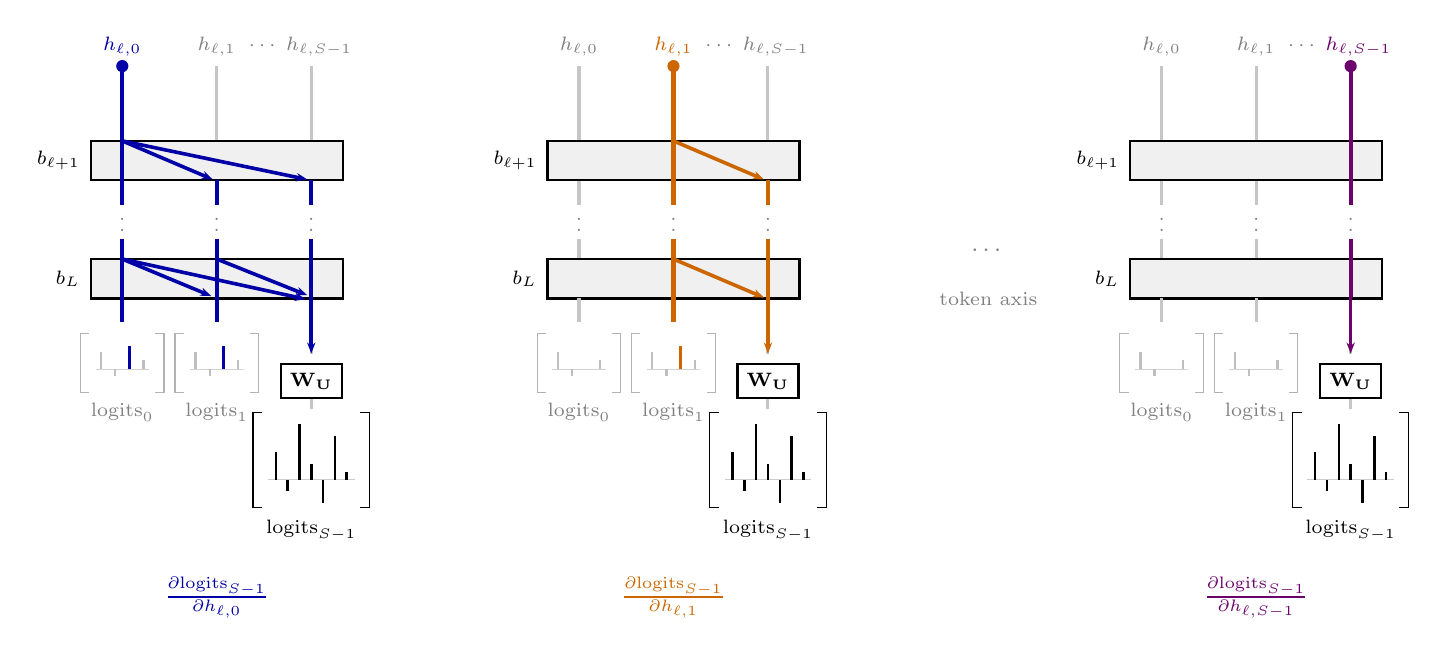
\begin{tikzpicture}[
  cord/.style={line width=1.1pt,gray!45},
  hcord/.style={line width=1.5pt,#1},
  harr/.style={line width=1.3pt,#1,-{Stealth[length=1.4mm]}},
]
%% Three panels, all happening at once: the (t, t' >= t) triangle the lens
%% averages over. Streams at x = -1.2 (pos 0), 0 (pos 1), 1.2 (pos S-1);
%% deliveries = diagonals inside blocks; vdots break every cord.
\foreach \panel/\PX in {0/0,1/5.8,2/13.2}{
\begin{scope}[xshift=\PX cm]
  \foreach \X in {-1.2,0,1.2}{
    \draw[cord] (\X,0.35) -- (\X,-0.6);
    \draw[cord] (\X,-1.1) -- (\X,-1.42);
    \node[jlabS,gray] at (\X,-1.63) {$\vdots$};
    \draw[cord] (\X,-1.84) -- (\X,-2.1);}
  \node[jlabS,gray] at (0.6,0.6) {$\cdots$};
  \node[draw,thick,fill=gray!12,minimum width=32mm,minimum height=5mm] (bA\panel) at (0,-0.85) {};
  \node[jlabS,left] at (bA\panel.west) {$b_{\ell+1}$};
  \node[draw,thick,fill=gray!12,minimum width=32mm,minimum height=5mm] (bB\panel) at (0,-2.35) {};
  \node[jlabS,left] at (bB\panel.west) {$b_{L}$};
  \draw[cord] (-1.2,-2.6) -- (-1.2,-2.9);
  \draw[cord] (0,-2.6) -- (0,-2.9);
  \draw[cord] (1.2,-2.6) -- (1.2,-3.3);
  \node[draw,thick,font=\scriptsize] (WU\panel) at (1.2,-3.65) {$\mathbf{W_U}$};
  \draw[cord] (WU\panel.south) -- (1.2,-4.0);
  \begin{scope}[shift={(1.2,-4.9)}]\jlogits{0}{0}\end{scope}
  \node[jlabS] at (1.2,-5.55) {$\logits_{S-1}$};
  % faint logits at the other positions (every stream admits unembedding)
  \foreach \mx/\mlab in {-1.2/{\logits_0},0/{\logits_1}}{
    \draw[gray!60] (\mx-0.42,-3.05) -| (\mx-0.53,-3.8) -- (\mx-0.42,-3.8);
    \draw[gray!60] (\mx+0.42,-3.05) -| (\mx+0.53,-3.8) -- (\mx+0.42,-3.8);
    \draw[gray!35,thin] (\mx-0.34,-3.5) -- (\mx+0.34,-3.5);
    \foreach \bi/\bv in {0/0.22,1/-0.09,3/0.12}{
      \draw[gray!50,line width=0.8pt] (\mx-0.27+\bi*0.18,-3.5) -- ++(0,\bv);}
    \node[jlabS,gray] at (\mx,-4.05) {$\mlab$};}
\end{scope}}
% ---- panel 1: h_{ell,0} floods every later stream and every logit
\begin{scope}
  \node[jlabS,blue!65!black] at (-1.2,0.6) {$h_{\ell,0}$};
  \node[jlabS,gray] at (0,0.6) {$h_{\ell,1}$};
  \node[jlabS,gray] at (1.3,0.6) {$h_{\ell,S-1}$};
  \fill[blue!65!black] (-1.2,0.35) circle (2.2pt);
  \draw[hcord=blue!65!black] (-1.2,0.35) -- (-1.2,-1.42);
  \draw[hcord=blue!65!black] (-1.2,-1.84) -- (-1.2,-2.6);
  \draw[hcord=blue!65!black] (-1.2,-2.6) -- (-1.2,-2.9);
  \draw[harr=blue!65!black] (-1.2,-0.6) -- (-0.05,-1.09);
  \draw[harr=blue!65!black] (-1.2,-0.6) -- (1.15,-1.09);
  \draw[hcord=blue!65!black] (0,-1.1) -- (0,-1.42);
  \draw[hcord=blue!65!black] (0,-1.84) -- (0,-2.6);
  \draw[hcord=blue!65!black] (0,-2.6) -- (0,-2.9);
  \draw[hcord=blue!65!black] (1.2,-1.1) -- (1.2,-1.42);
  \draw[hcord=blue!65!black] (1.2,-1.84) -- (1.2,-2.6);
  \draw[harr=blue!65!black] (-1.2,-2.1) -- (-0.07,-2.57);
  \draw[harr=blue!65!black] (-1.2,-2.1) -- (1.13,-2.61);
  \draw[harr=blue!65!black] (0,-2.1) -- (1.15,-2.56);
  \draw[harr=blue!65!black] (1.2,-2.6) -- (1.2,-3.3);
  \draw[blue!65!black,line width=1pt] (-1.2+0.09,-3.5) -- ++(0,0.3);
  \draw[blue!65!black,line width=1pt] (0.09,-3.5) -- ++(0,0.3);
  \node[jlab,blue!65!black] at (0,-6.4) {$\frac{\partial \logits_{S-1}}{\partial h_{\ell,0}}$};
\end{scope}
% ---- panel 2: h_{ell,1} reaches its own and later logits, never position 0
\begin{scope}[xshift=5.8cm]
  \node[jlabS,gray] at (-1.2,0.6) {$h_{\ell,0}$};
  \node[jlabS,orange!80!black] at (0,0.6) {$h_{\ell,1}$};
  \node[jlabS,gray] at (1.3,0.6) {$h_{\ell,S-1}$};
  \fill[orange!80!black] (0,0.35) circle (2.2pt);
  \draw[hcord=orange!80!black] (0,0.35) -- (0,-1.42);
  \draw[hcord=orange!80!black] (0,-1.84) -- (0,-2.6);
  \draw[hcord=orange!80!black] (0,-2.6) -- (0,-2.9);
  \draw[harr=orange!80!black] (0,-0.6) -- (1.15,-1.09);
  \draw[hcord=orange!80!black] (1.2,-1.1) -- (1.2,-1.42);
  \draw[hcord=orange!80!black] (1.2,-1.84) -- (1.2,-2.6);
  \draw[harr=orange!80!black] (0,-2.1) -- (1.15,-2.59);
  \draw[harr=orange!80!black] (1.2,-2.6) -- (1.2,-3.3);
  \draw[orange!80!black,line width=1pt] (0.09,-3.5) -- ++(0,0.3);
  \node[jlab,orange!80!black] at (0,-6.4) {$\frac{\partial \logits_{S-1}}{\partial h_{\ell,1}}$};
\end{scope}
% ---- panel 3: h_{ell,S-1}, the straight shot; only its own logits
\begin{scope}[xshift=13.2cm]
  \node[jlabS,gray] at (-1.2,0.6) {$h_{\ell,0}$};
  \node[jlabS,gray] at (0,0.6) {$h_{\ell,1}$};
  \node[jlabS,violet!85!black] at (1.3,0.6) {$h_{\ell,S-1}$};
  \fill[violet!85!black] (1.2,0.35) circle (2.2pt);
  \draw[hcord=violet!85!black] (1.2,0.35) -- (1.2,-1.42);
  \draw[hcord=violet!85!black] (1.2,-1.84) -- (1.2,-2.6);
  \draw[harr=violet!85!black] (1.2,-2.6) -- (1.2,-3.3);
  \node[jlab,violet!85!black] at (0,-6.4) {$\frac{\partial \logits_{S-1}}{\partial h_{\ell,S-1}}$};
\end{scope}
% ellipsis over the token axis, between panel 1 and panel S-1
\node[jlab,gray] at (9.8,-2.0) {$\cdots$};
\node[jlabS,gray,align=center] at (9.8,-2.6) {token axis};
\end{tikzpicture}}
\caption{This figure depicts the \textit{S} \textit{source} latents that affect the final \(\logits_{S-1}\) vector. These three panels are happening \textit{at once}. Each activation deposits some causal influence on \textit{all} logit vectors succeeding it.}
\label{fig:context-strip}
\end{figure}

\begin{figure}[htbp]
\centering
\resizebox{0.8\textwidth}{!}{%
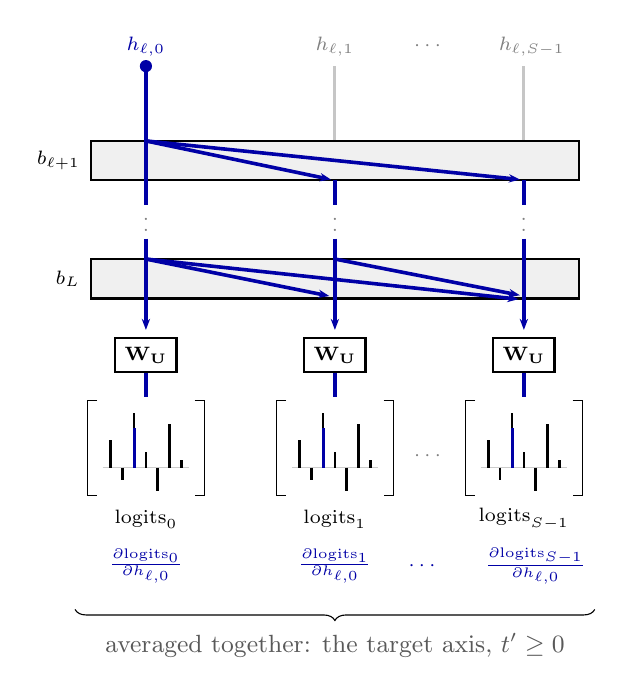
\begin{tikzpicture}[
  cord/.style={line width=1.1pt,gray!45},
  hcord/.style={line width=1.5pt,#1},
  harr/.style={line width=1.3pt,#1,-{Stealth[length=1.4mm]}},
]
\def\hc{blue!65!black}
% streams and stack (wide: full charts and one-row Jacobians below)
\foreach \X in {-2.4,0,2.4}{
  \draw[cord] (\X,0.35) -- (\X,-0.6);
  \draw[cord] (\X,-1.1) -- (\X,-1.42);
  \node[jlabS,gray] at (\X,-1.63) {$\vdots$};
  \draw[cord] (\X,-1.84) -- (\X,-2.1);}
\node[jlabS,gray] at (1.2,0.6) {$\cdots$};
\node[jlabS,\hc] at (-2.4,0.6) {$h_{\ell,0}$};
\node[jlabS,gray] at (0,0.6) {$h_{\ell,1}$};
\node[jlabS,gray] at (2.5,0.6) {$h_{\ell,S-1}$};
\node[draw,thick,fill=gray!12,minimum width=62mm,minimum height=5mm] (fA) at (0,-0.85) {};
\node[jlabS,left] at (fA.west) {$b_{\ell+1}$};
\node[draw,thick,fill=gray!12,minimum width=62mm,minimum height=5mm] (fB) at (0,-2.35) {};
\node[jlabS,left] at (fB.west) {$b_{L}$};
% the tapped latent floods every stream...
\fill[\hc] (-2.4,0.35) circle (2.2pt);
\draw[hcord=\hc] (-2.4,0.35) -- (-2.4,-1.42);
\draw[hcord=\hc] (-2.4,-1.84) -- (-2.4,-2.6);
\draw[harr=\hc] (-2.4,-0.6) -- (-0.05,-1.09);
\draw[harr=\hc] (-2.4,-0.6) -- (2.35,-1.09);
\draw[hcord=\hc] (0,-1.1) -- (0,-1.42);
\draw[hcord=\hc] (0,-1.84) -- (0,-2.6);
\draw[hcord=\hc] (2.4,-1.1) -- (2.4,-1.42);
\draw[hcord=\hc] (2.4,-1.84) -- (2.4,-2.6);
\draw[harr=\hc] (-2.4,-2.1) -- (-0.07,-2.57);
\draw[harr=\hc] (-2.4,-2.1) -- (2.33,-2.61);
\draw[harr=\hc] (0,-2.1) -- (2.35,-2.56);
% ...and every stream admits the (shared) unembedding
\foreach \X/\tl in {-2.4/{\logits_0},0/{\logits_1},2.4/{\logits_{S-1}}}{
  \draw[harr=\hc] (\X,-2.6) -- (\X,-3.0);
  \node[draw,thick,font=\scriptsize] at (\X,-3.32) {$\mathbf{W_U}$};
  \draw[hcord=\hc] (\X,-3.55) -- (\X,-3.85);
  \begin{scope}[shift={(\X,-4.75)}]\jlogits{0}{0}\end{scope}
  \draw[\hc,line width=1.1pt] (\X-0.15,-4.75) -- ++(0,0.5);
  \node[jlabS] at (\X,-5.4) {$\tl$};}
\node[jlabS,gray] at (1.2,-4.6) {$\cdots$};
% the row of Jacobians this fan produces
\node[jlabS,\hc] at (-2.4,-6.0) {$\frac{\partial \logits_0}{\partial h_{\ell,0}}$};
\node[jlabS,\hc] at (0,-6.0) {$\frac{\partial \logits_1}{\partial h_{\ell,0}}$};
\node[jlabS,\hc] at (1.13,-6.0) {$\cdots$};
\node[jlabS,\hc] at (2.55,-6.0) {$\frac{\partial \logits_{S-1}}{\partial h_{\ell,0}}$};
\draw[decorate,decoration={brace,mirror,amplitude=4pt}] (-3.3,-6.55) -- (3.3,-6.55)
      node[midway,below=5pt,jlab,gray!70!black]{averaged together: the target axis, $t' \ge 0$};
\end{tikzpicture}}
\caption{The complement to Figure~\ref{fig:context-strip}. Here, we highlight not the activations affecting a single logit vector, but a single activation and the many logit vectors it influences. One latent, $h_{\ell,0}$, and every logit vector it touches---its causal \textit{tails}.}
\label{fig:fan-out}
\end{figure}


Averaging over token position for a single context \(c_{\mathscr{p}}\)'s latents gives us the mean influence of layer \(\ell\) latents on future layer \(L\) latents.\footnote{It should be made clear that while there are 5050 distinct relationships being averaged together in the above example, we only need \(\dmodel\) iterations to compute this mean for the whole context \(\mathbf{C}_{\mathscr{p}}\). A forward pass seeded at layer \(\ell\) propagates to \textit{all} downstream positions in a single sweep, and the causal mask guarantees a source latent \(h_{\ell,t}\) reaches only targets \(t' \ge t\). So \(\dmodel\) forward probes---one per model dimension---already carry every source's influence to every target it can touch, filling the whole-context Jacobian without ever visiting the 5050 pairs one at a time.}

\[J^{\mathscr{p}}_\ell = \mathbb{E}_{t \le t' < S_{\mathscr{p}}}\left[\frac{\partial h_{L,t'}}{\partial h_{\ell,t}}\right] = \mathbb{E}_{t \le t' < S_{\mathscr{p}}}\left[\frac{\partial R_\ell}{\partial h_{\ell}}\right]\]

Averaging \(|\mathscr{P}|\) of these context-specific Jacobians \(J^{\mathscr{p}}_\ell\) gives us \(J_\ell\).

\[J_\ell = \mathbb{E}_{\mathscr{p} \in \mathscr{P}}\left[J^{\mathscr{p}}_\ell\right]\]

As we saw in the definition above, with \(J_\ell\), we have \(\jlens_\ell\). Composition with \(\mathbf{W_U}\) is the static readout lens for layer \(L\) latents and \(J_\ell\) already approximates the translation from layer \(\ell\). We've tied the directions of layer \(\ell\) latents through layer \(L\) latents to tokens, at positions \(t' \ge t\). This gives \(\jlens\) bearing over future---not past, and not just \textit{immediate} future---verbalization. \footnote{To indulge intuitions about what the \(\jlens\) object is, we should mention that it can be equivalently computed in \(|V|\) \textit{backward} passes as opposed to \(\dmodel\) \textit{forward} passes per context. \(\jlens\) is a full \(\mathbb{R}^{|V| \times \dmodel}\) matrix and it can be iteratively filled by columns (\(\dmodel\) steps) or by rows (\(|V|\) steps). In most LLMs, \(|V|\) is larger than \(\dmodel\), suggesting that we'd be better off going forward and looping only \(\dmodel\) times. But beyond that, in order to fill \(\jlens\) row-by-row, you must differentiate back through \(\mathbf{W_U}\) in every step, even though it is a static matrix---a plain waste of compute. What these expected Jacobians (\(J\) and \(\jlens\)) really bring to the table is an approximation of the expected Jacobian of the \textit{nonlinear} processing of the network. Being a static matrix, \(\mathbf{W_U}\) \textit{is} its own Jacobian. In the typical \(\dmodel\)-iterations case, we do our passes from layer \(\ell\) to \(L\), always going from \(\mathbb{R}^{\dmodel} \to \mathbb{R}^{\dmodel}\), working hard to probe the nonlinearity and nothing else. In the same vein as the column-wise fill, if we wanted to do \(|V|\) row-wise backward passes, we would seed each one with a standard basis vector \(e_v \in \mathbb{R}^{|V|}\) to get each \(v\)-th row of \(\jlens\). Figure~\ref{fig:two-modes} shows the mirror equivalence of the forward (filling each of the \(\dmodel\) columns of \(\jlens\)) and backward (filling each of the \(|V|\) rows of \(\jlens\)) methods and why they're equivalent. } 




\subsection{Insightful Caveats}
What is the epistemological cost of averaging the local Jacobians into a global lens? An individually computed \(\frac{\partial h_{L,t'}}{\partial h_{\ell,t}} \in \mathbb{R}^{\dmodel \times \dmodel}\) is exact, but indexed to a specific point in layer \(\ell\)'s activation space. The earlier \(\ell\) is, the more of \(R_{\ell}\)'s higher-order curvature is being averaged away when we mean---first over positions into each context's \(J^{\mathscr{p}}_{\ell}\) and then over \(|\mathscr{P}|\) contexts---into the single \(J_{\ell}\). We average a layer's map over all (\(|\mathscr{P}| \times S\)) visited activations, pretending like local linear behavior is shared regionally when it really isn't. Figure~\ref{fig:tangents} attempts to stimulate intuitions about the information lost in local linear averaging of non-linear functions.

So then why average over contexts if we're creating an increasingly approximated object by doing so? The goal of \(\jlens\) is not to be an exact \(J\) of a specific \(\logits\) vector, with respect to a specific \(h\)---it is manifestly to be an aggregated, generalized map. While the complexity of the field of local functions defined in \(F\) (by way of \(R\))---the distinct attention paid to every unique context---is exactly what makes these models so powerful, the construction of \(\jlens\) is a \textit{postulation} that there is \textit{some} shared shape across the ways each context inspires speech in the model. Complex as \(F\) necessarily is, it is not some incompressibly arbitrary map.\footnote{Don't you feel that, even though every facial expression you've made is the outcome of a unique circumstance, there might still be an average relationship your best friend could use to predict how you feel and how you may act? Transformers have no faces, they have latent activations; interpretability researchers armed with calculus are the knowing friends who seek to learn their behavior. But your friend doesn't study the physics of your facial expressions to learn how they entail behavior---they build an averaged, general mapping between facial expression, mood, and your behavior.} We lose information when we average local specificity into regional (dare we say) global approximations, but what we retain has general, nontrivial causal insight (as the \href{https://transformer-circuits.pub/2026/workspace/index.html}{paper} shows and we discuss in \S\ref{sec:jfindings}).\footnote{For what it is worth, \textit{training} adheres to the same postulation with respect to the effect of averaging over nonlinearity. It is hard to deny its success in postulating so. \(\jlens\) takes the same kinds of means and shows that---in the trained model, in \textit{activation} space---specificity is not the entire story.}

Averaging is a hypothesis. Here is how we test it: we can measure the magnitude of difference (\(\delta_{\ell,t,t'} = \left\|\frac{\partial h_{L,t'}}{\partial h_{\ell,t}} - J_\ell\right\|^2\)) between each local Jacobian and the global \(J_\ell\), and then average this to get an overall expected \textbf{dispersion} measure (\(\dispersion_\ell = \mathbb{E}_{t' \ge t,\, \mathscr{P}}[\delta_{\ell,t,t'}]\))\footnote{By the law of total variance the total splits as \(\dispersion_\ell = \dispersion^{\mathrm{w}}_\ell + \dispersion^{\mathrm{b}}_\ell\): a \textit{within-context} part \(\dispersion^{\mathrm{w}}_\ell = \mathbb{E}_{\mathscr{p}}\,\mathbb{E}_{t'\ge t}\bigl\lVert\frac{\partial h_{L,t'}}{\partial h_{\ell,t}} - J^{\mathscr{p}}_\ell\bigr\rVert^2\) (atoms scattering around their own prompt's mean---local curvature) plus a \textit{between-context} part \(\dispersion^{\mathrm{b}}_\ell = \mathbb{E}_{\mathscr{p}}\bigl\lVert J^{\mathscr{p}}_\ell - J_\ell\bigr\rVert^2\) (prompt-means disagreeing). We headline the total, but the between-part is the sharper object---it alone asks whether averaging \textit{over contexts} was warranted, i.e.\ how well the lens generalizes across them. The identity is exact provided both stages share one weighting over contexts: automatic for uniform \(S_{\mathscr{p}}\), and for mixed lengths one weights each context by its \((t,t')\) pair-count.} for a given \(J_\ell\).\footnote{Since the readout \(\mathbf{W_U}\) is a shared constant, it drops out of the difference, and only the nonlinear transport actually varies.} \(\dispersion_\ell\) is proportional to (1) the higher-order curvature of \(R_{\ell}\) and (2) variance in the sampled activations \(h_\ell\) in the \(h\)-region sampled. These factors compound, schematically: \(\dispersion_\ell \;\propto\; \left\|\frac{\partial^2 R_\ell}{\partial h_\ell^2}\right\|^2 \cdot \mathbb{E}\|h_\ell-\bar h_\ell\|^2\).


\(\dispersion\) fills in the detail productively smeared by \(J\) and \(\jlens\), complementing but not invalidating their causal importance.\footnote{Good, knowing friendships are not based on facial physics!}

%% The lens as the mean of tangents. Reference as Figure~\ref{fig:tangents}.
\begin{figure}[htbp]
\centering
\resizebox{0.8\textwidth}{!}{%
\begin{tikzpicture}[scale=1.35]
% axes
\draw[-{Stealth[length=1.8mm]}] (-0.2,0) -- (6.9,0);
\draw[-{Stealth[length=1.8mm]}] (0,-0.3) -- (0,2.6) node[jlabS,above] {$R_\ell(h)$ \scriptsize(one coord.\ of $h_L$)};
% the true nonlinear map
\draw[thick] plot[smooth] coordinates {(0.20,0.181) (0.41,0.365) (0.62,0.533) (0.83,0.681) (1.04,0.803) (1.25,0.895) (1.46,0.956) (1.67,0.984) (1.88,0.983) (2.09,0.955) (2.30,0.906) (2.51,0.842) (2.72,0.769) (2.93,0.696) (3.14,0.630) (3.35,0.579) (3.56,0.549) (3.77,0.544) (3.98,0.569) (4.19,0.626) (4.40,0.715) (4.61,0.834) (4.82,0.979) (5.03,1.145) (5.24,1.327) (5.45,1.517) (5.66,1.708) (5.87,1.891) (6.08,2.060) (6.29,2.209) (6.50,2.331)};
\node[jlabS,right] at (6.45,2.32) {$R_\ell$};
% per-context tangents at the visited activations
\draw[gray!55,thin] (1.00,0.956) -- (2.40,1.016);
\draw[gray!55,thin] (1.30,1.069) -- (2.70,0.871);
\draw[gray!55,thin] (1.55,1.100) -- (2.95,0.739);
\draw[gray!55,thin] (1.80,1.076) -- (3.20,0.614);
\draw[gray!55,thin] (2.05,1.005) -- (3.45,0.512);
\draw[gray!55,thin] (2.30,0.899) -- (3.70,0.447);
\draw[gray!55,thin] (2.65,0.719) -- (4.05,0.440);
\draw[gray!55,thin] (3.20,0.460) -- (4.60,0.652);
\fill (1.70,0.986) circle (1.3pt);
\fill (2.00,0.970) circle (1.3pt);
\fill (2.25,0.919) circle (1.3pt);
\fill (2.50,0.845) circle (1.3pt);
\fill (2.75,0.759) circle (1.3pt);
\fill (3.00,0.673) circle (1.3pt);
\fill (3.35,0.579) circle (1.3pt);
\fill (3.90,0.556) circle (1.3pt);
% the mean of the tangents: the lens
\draw[jvio,line width=1.3pt] (0.5,1.171) -- (6.1,0.174);
\node[jlabS,jvio,right] at (6.15,0.36) {$J_\ell$: the mean tangent};
% where the line lies
\draw[gray!60,dashed] (5.4,0.299) -- (5.4,1.472);
\fill[gray!60] (5.4,1.472) circle (1.1pt);
\node[jlabS,gray!70!black,align=center,right] at (5.52,1.0) {far from the data,\\the line lies};
% dispersion note
\node[jlabS,gray!70!black,align=center] at (1.35,2.15) {curvature makes the\\tangents disagree:\\\emph{dispersion}};
\draw[gray!60,thin,-{Stealth[length=1.3mm]}] (1.75,1.85) to[out=-60,in=140] (2.42,1.05);
% ==== dispersion strip: shared h-axis, F and mean removed, delta bars added ====
% faint droplines: each dot above sits directly over its delta bar below (shared h)
\foreach \x/\bt in {1.70/-1.561,2.00/-1.988,2.25/-1.943,2.50/-1.792,2.75/-1.727,3.00/-1.811,3.35/-1.996,3.90/-1.106}{
  \draw[gray!30,thin,dotted] (\x,-0.12) -- (\x,\bt);}
% the bars: delta_i = || J_ell(h_i) - J_ell ||^2, at the same x as each dot above
\foreach \x/\h in {1.70/0.439,2.00/0.012,2.25/0.057,2.50/0.208,2.75/0.273,3.00/0.189,3.35/0.004,3.90/0.894}{
  \fill[jvio!72] (\x-0.055,-2.0) rectangle (\x+0.055,{-2.0+\h});}
% net dispersion = mean bar height, full width
\draw[jvio,dashed,line width=1pt] (0,-1.741) -- (6.9,-1.741);
\node[jlabS,jvio,above] at (5.5,-1.735) {$\dispersion_\ell=\mathbb{E}[\delta]\approx0.029$};
\node[jlabS,gray!70!black,align=center] at (5.15,-1.12) {this context's $\delta$\\ dominates};
\draw[gray!55,thin,-{Stealth[length=1.2mm]}] (4.45,-1.16) to[out=180,in=55] (3.99,-1.18);
% delta-axis (black) at x=0, colinear with the top y-axis
\draw[-{Stealth[length=1.8mm]}] (0,-2.06) -- (0,-0.88) node[jlabS,above left=0pt] {$\delta(h)$};
\node[jlabS,left] at (-0.06,-2.0) {$0$};
% the shared x-axis (black), labeled here beneath the lower panel
\draw[-{Stealth[length=1.8mm]}] (-0.2,-2.0) -- (6.9,-2.0) node[jlabS,below left=1pt] {$h$ \scriptsize(one direction of $\mathbb{R}^{\dmodel}$)};
% region annotation, now beneath the shared axis
\draw[decorate,decoration={brace,mirror,amplitude=3pt}] (1.55,-2.18) -- (4.05,-2.18)
      node[midway,below=3pt,jlabS,gray!70!black] {region visited by real activations};
\end{tikzpicture}}
\caption{What the lens is: the average of the local linear behaviors $J_\ell(h) = \frac{\partial h_L}{\partial h}$---i.e.\ the atom $\frac{\partial h_{L,t'}}{\partial h_{\ell,t}}$ at each visited latent $h = h_{\ell,t}$---across the activations the model actually visits (dots; one gray tangent each). Where $R_\ell$ curves within the visited region, the tangents fan---that spread \emph{is} the dispersion $\dispersion_\ell = \mathbb{E}\|J_\ell(h)-J_\ell\|^2$. And the mean tangent is a local instrument: far from the sampled region, the line and the function part ways. The lower panel makes the spread concrete: each bar is one visited latent's $\delta = \|J_\ell(h)-J_\ell\|^2$---how far its tangent tilts from the mean---and $\dispersion_\ell$ is simply their average, pulled up here by the lone high-curvature latent at the region's right edge.}
\label{fig:tangents}
\end{figure}



\section{J-space}\label{sec:jspace}

Where \(\jlens\) shines in the \textit{synthesis} it makes of causal relationships into a single object, it blinds with its potent density. The \textbf{J-space} is a kind of prism we fit to the information that pours into \(\jlens\), reducing it to its principal components and focusing its information into distinct beams of practical insight. \(\jlens\) colors the \(\dmodel\)-sized latent states of the model with what it means for all \(|V|\) concepts in its available grasp, but do we feel intuitively that every thought in our heads should be put in relation to \textit{every} word we can possibly utter? Any \(h\) must be reducible to only those directions in token space that really count, right? Beyond the reduction the \textbf{J-space} provides for the purposes of interpreting internal state, if we want to affect change in the model's behavior, we'd hope that we wouldn't have to tweak \textit{every single} source, but only a privileged few, right? 

Knowing the normalized alignment vector \(\jlens(h)\) of any latent is valuable, but \(\jlens\) itself (and the vocabulary it speaks to!) is highly redundant. If \(h\) scores highly with an (imaginary) token, ``dog'', then it will likely align with tokens such as ``dogs'', ``canine'', and ``puppy''. Knowing one of these practically tells us the other. Taking the top 10 scoring tokens from \(\jlens(h)\) might only give us 2 or 3 truly distinct concepts.

The \textbf{J-space} \(\jspace\) is defined to bring information-retaining \textbf{sparsity} to the redundancy of \(\jlens\)-space. \(\jspace\) is an \textit{intensionally} as opposed to \textit{extensionally} defined space, never fully enumerated as an object like \(\jlens\) but instead specified by a constrained recipe for finding its members.\footnote{For one thing, it is an \textit{uncountably} infinite space---a union of finitely many cones, but each cone a continuum of points---so we could never compact it into an object like \(\jlens\).} The \textbf{J-space} \textit{decomposition} \(\jspace(h)\) of an activation \(h\) is the closest point \textit{in the \textbf{J-space}} to \(h\) itself.

Once \(\jlens\)-space is made sparse, the meaningful conceptual decomposition of the residual stream is fast-tracked and principled, allowing for efficiently pointed interventions. The torrential information delivered in \(\jlens\) gets its due scrutiny, allowing us to isolate and utilize its (literally) most pointed insights. 

\subsection{Computation}\label{sec:jspacecomp}

The \textbf{J-space} \(\jspace_\ell\) in layer \(\ell\) is defined as the set of all points reachable by a sparse, nonnegative decomposition of up to \(k\) rows of \(\jlens\), where \(k\) is our sparsity constraint. Anthropic denotes it as a \textit{union of cones} in \(\mathbb{R}^{\dmodel}\), where each cone is made up of a set of \(k\) directions (rows drawn from \(\jlens\)), each with a nonnegative coefficient. Writing \(\mathscr{m}_{v}\) for the row of \(\jlens\) belonging to token \(v\), and collecting the coefficients into a single sparse, nonnegative vector \(c \in \mathbb{R}^{|V|}_{\ge 0}\) with at most \(k\) nonzero entries (\(\|c\|_0 \le k\)), the space is
\[ \jspace \;=\; \bigl\{\, \jlens^{\!\top} c \;:\; c \ge 0,\ \|c\|_0 \le k \,\bigr\}, \qquad \jlens^{\!\top} c \;=\; \sum_{v=1}^{|V|} c_v\, \mathscr{m}_{v} \]

The \textbf{J-space} \textit{component} \(\jspace(h)\) of a latent \(h\) is then defined as the point in \(\jspace\) that is closest to \(h\).

\[ \jspace(h) \;=\; \jlens^{\!\top} c^\star, \qquad c^\star \;=\; \argmin_{\substack{c \,\in\, \mathbb{R}^{|V|}_{\ge 0} \\ \|c\|_0 \,\le\, k}} \bigl\| \jlens^{\!\top} c - h \bigr\|_2^2  \]

\(c^\star\) is our prism on the overcomplete white light that is \(\jlens\). Once fit, \(c^\star\)  sifts the principal directions in \(\jlens\)-space (\(\in \mathbb{R}^{\dmodel}\)) that best reconstruct \(h\). If each row of \(\jlens\) denotes a direction of steepest logit-increase for each token, then \(\jspace(h)\) puts together a non-redundant report of the \(k\) directions in token space that best describe the model's disposition.

While the notation defining \(\jspace(h)\) is succinct, choosing the best \(k\) rows out of a \(|V|\)-term dictionary is NP-hard, so we solve it greedily. One objective---\textit{reconstruct \(h\) as closely as possible with only \(k\) rows}---forces two oscillating complementary operations: \textit{select} directions against the residual \(r\) (which progressively shrinks during the optimization), but always \textit{fit} against \(h\). Every \textit{next} direction \(\mathscr{m}\) is the one most aligned with \textit{what still needs to be covered} (the residual, \(r\)). After each next direction selection, we see how well the working set of directions reconstructs the ultimate objective, \textit{h}. \textit{Diversity} among the \(k\) rows of \(\jlens\) that we select is never an imposed rule---it falls out of greedily \textit{selecting} against the residual but \textit{fitting} against the target. The selected rows are not thereby mutually \textit{orthogonal} (with an overcomplete, correlated dictionary they generally are not); what emerges is only that we never spend a slot re-selecting a direction the working set already covers, since after each refit the residual is (near-)orthogonal to everything we have already captured. Algorithm~\ref{alg:jspace} displays the \textit{outer} algorithm for selecting directions, while Algorithm~\ref{alg:fit} specifies how those directions are fit. Because \textsc{Fit} re-solves \textit{all} of the active coefficients against \(h\) at every round---rather than freezing past coefficients and only appending the new one---the procedure is, strictly, \textit{orthogonal} matching pursuit (in fact its nonnegative variant), not the original matching pursuit.\footnote{Orthogonal matching pursuit: Y.~C. Pati, R.~Rezaiifar, and P.~S. Krishnaprasad, \textit{Orthogonal Matching Pursuit: Recursive Function Approximation with Applications to Wavelet Decomposition}, Proc.\ 27th Asilomar Conf.\ on Signals, Systems and Computers, \href{https://doi.org/10.1109/ACSSC.1993.342465}{1993}. The refit is what makes it \textit{orthogonal}: after it, the residual is orthogonal to the span of the active rows.}

% ===== J-space decomposition algorithm (matching pursuit + refit) =====
% Reference it in prose as: Algorithm~\ref{alg:jspace}  (renders "Algorithm 1", clickable via hyperref).
% This is a working draft --- fill in / adjust the steps, comments, and any stopping rule as you like.
\begin{algorithm}[htbp]
\caption{\(\jspace(h)\)}
\label{alg:jspace}
\begin{algorithmic}[1]
\Require latent \(h \in \mathbb{R}^{\dmodel}\);\ \ J-lens rows \(\mathscr{m}_{v}\) for \(v = 0,\dots,|V|-1\);\ \ sparsity budget \(k\)
\Ensure sparse nonnegative \(c \in \mathbb{R}^{|V|}_{\ge 0}\) with \(\|c\|_0 \le k\);\ \ component \(\jspace(h) = \jlens^{\!\top} c\)
\State \(r \gets h\);\quad \(A \gets \varnothing\);\quad \(c \gets \mathbf{0}\) \Comment{residual, active support, coefficients}
\For{\(j = 1\) \textbf{to} \(k\)} \Comment{outer loop: grow the support}
  \State \(\displaystyle v^\star \gets \argmax_{v}\ \frac{\langle \mathscr{m}_{v},\, r\rangle}{\lVert \mathscr{m}_{v}\rVert}\) \Comment{select against the residual \(r\) --- the fastest error drop}
  \State \(A \gets A \cup \{v^\star\}\) \Comment{selecting against \(r\), not \(h\), keeps the support diverse}
  \State \(c_A \gets\) \textsc{Fit}\((A, h)\) \Comment{fit the weights against \(h\) itself (Alg.~\ref{alg:fit})}
  \State \(\displaystyle r \gets h - \sum_{v \in A} (c_A)_v\, \mathscr{m}_{v}\) \Comment{what \(\jspace\) still cannot explain}
\EndFor
\State \Return \(c\) (zero off \(A\)),\ \ \(\jspace(h) = \jlens^{\!\top} c\)
\end{algorithmic}
\end{algorithm}

% ===== The inner fit, called from Algorithm 1 line 5. Reference as Algorithm~\ref{alg:fit}. =====
% Convergence story: projected gradient descent, run until the residual stops shrinking.
% NOTE: the gradient g_v = -<m_v, r> is the SAME alignment-with-residual used to SELECT in Alg 1 ---
% selection picks the single most-aligned row; the fit nudges every active row by its alignment.
\begin{algorithm}[htbp]
\caption{\textsc{Fit}\((A, h)\)}
\label{alg:fit}
\begin{algorithmic}[1]
\Require active support \(A\); latent \(h\); J-lens rows \(\mathscr{m}_{v}\); step size \(\eta\)
\Ensure \(c_A \ge 0\) minimizing \(\bigl\lVert \sum_{v \in A}(c_A)_v\,\mathscr{m}_{v} - h \bigr\rVert_2^2\)
\State \(c_A \gets \mathbf{0}\)
\Repeat
  \State \(\displaystyle r \gets h - \sum_{v \in A}(c_A)_v\,\mathscr{m}_{v}\) \Comment{residual under the current weights}
  \State \(g_v \gets -\langle \mathscr{m}_{v},\, r\rangle \quad \forall\, v \in A\) \Comment{gradient: (minus) each row's alignment with \(r\)}
  \State \(c_A \gets \max\!\bigl(\mathbf{0},\; c_A - \eta\, g\bigr)\) \Comment{descend, then project back onto \(c_A \ge 0\)}
\Until{\(\lVert r\rVert\) stops shrinking}
\State \Return \(c_A\)
\end{algorithmic}
\end{algorithm}


Algorithm~\ref{alg:fit} should seem familiar: it is gradient descent! Write the error as \(e \equiv \hat{s} - h = \sum_w c_w\, m_w - h = -r\), so the loss is
\[ L(c) \;=\; \bigl\lVert \hat{s} - h\bigr\rVert_2^2 \;=\; \lVert e\rVert^2 \;=\; e \cdot e \]
Differentiating with respect to a single coefficient \(c_v\),
\[ \frac{\partial L}{\partial c_v} \;=\; \frac{\partial}{\partial c_v}\,\bigl(e \cdot e\bigr) \;=\; 2\, e \cdot \frac{\partial e}{\partial c_v}. \]
The inner derivative picks out a single term,
\[ \frac{\partial e}{\partial c_v} \;=\; \frac{\partial}{\partial c_v}\Bigl(\sum_w c_w\, m_w - h\Bigr) \;=\; m_v \]
since \(h\) and every \(c_w\) with \(w \neq v\) are constant in \(c_v\). Substituting back,
\[ \frac{\partial L}{\partial c_v} \;=\; 2\, e \cdot m_v \;=\; 2(\hat{s}-h)\cdot m_v \;=\; 2(-r)\cdot m_v \;=\; -2\,\langle m_v,\, r\rangle \]

At every turn of the optimization, \(r\) is the vector representing all of \(h\) that we have not reconstructed. It is a \textit{direction} in which we want to move, not a point at which we want to arrive. The more we nudge \(\sum_{v \in A}(c_A)_v\,\mathscr{m}_{v}\) towards \(r\), the more \(r\) disappears.\footnote{Because \(r = h - \sum_{v \in A}(c_A)_v\,\mathscr{m}_{v}\)!} We want to adjust each coefficient \(c_v\) so it supports this directional goal and brings its corresponding \(\mathscr{m}_v\) to where it needs to be to cancel more of \(r\). What is the relationship between \(c_v\) and \(r\)? It is exactly (proportional to) \(\langle m_v,\, r\rangle\)!

The motivation for the \textbf{J-space} decomposition \(\jspace(h)\) of a latent \(h\) is plain: positively include the \(k\) distinct token-influence directions of \(h\)-space that can reconstruct \(h\) the best. The \textit{algorithm} for computing it, though, is even more plain and elegant. At every turn of the outer algorithm, select the direction that best eats up the work we have left to do (\(r\))---this is what buys us the diversity noted above. Then for each working set of directions, figure out the best way to combine them to reconstruct the information we actually want to reconstruct, \(h\). The algorithm is so nice because its goal is so interpretable and intuitive and its methods are so familiar to anyone who has worked with neural networks. Interestingly, it was originally introduced (under the name of \textit{matching pursuit}) in the context of continuous signal processing by Mallat and Zhang \href{https://doi.org/10.1109/78.258082}{(1993)}.\footnote{S.~G. Mallat and Z.~Zhang, \textit{Matching Pursuits with Time-Frequency Dictionaries}, IEEE Trans.\ Signal Processing, 41(12):3397--3415, 1993.} Continuous sinusoidal waves that are composed of pure frequencies, each at a specific coefficient (and phase), resemble vectors that are composed of different directions. The motivation to deconstruct them is the same: \textit{which frequencies are present in this signal?} Better yet, \textit{what are the top k frequencies that could approximate this signal?} Each pure frequency brings something distinct to the table, like each orthogonal direction of a vector space. How do you find the single pure frequency that best aligns with a sinusoid (be it a raw signal or a residual!)? Dot product, Discrete Fourier Transform. If you have a set of choice pure frequencies, how do you you figure out their best combination to reconstruct a sinusoid? Gradient descent!  Figure~\ref{fig:jspace-freq} celebrates this alignment in methods and motivations, honoring the original instantiation of the matching pursuit algorithm which we use to compute \(\jspace(h)\), and stimulating your intuition for what reconstruction really looks like. 

\begin{figure}[htbp]
\centering
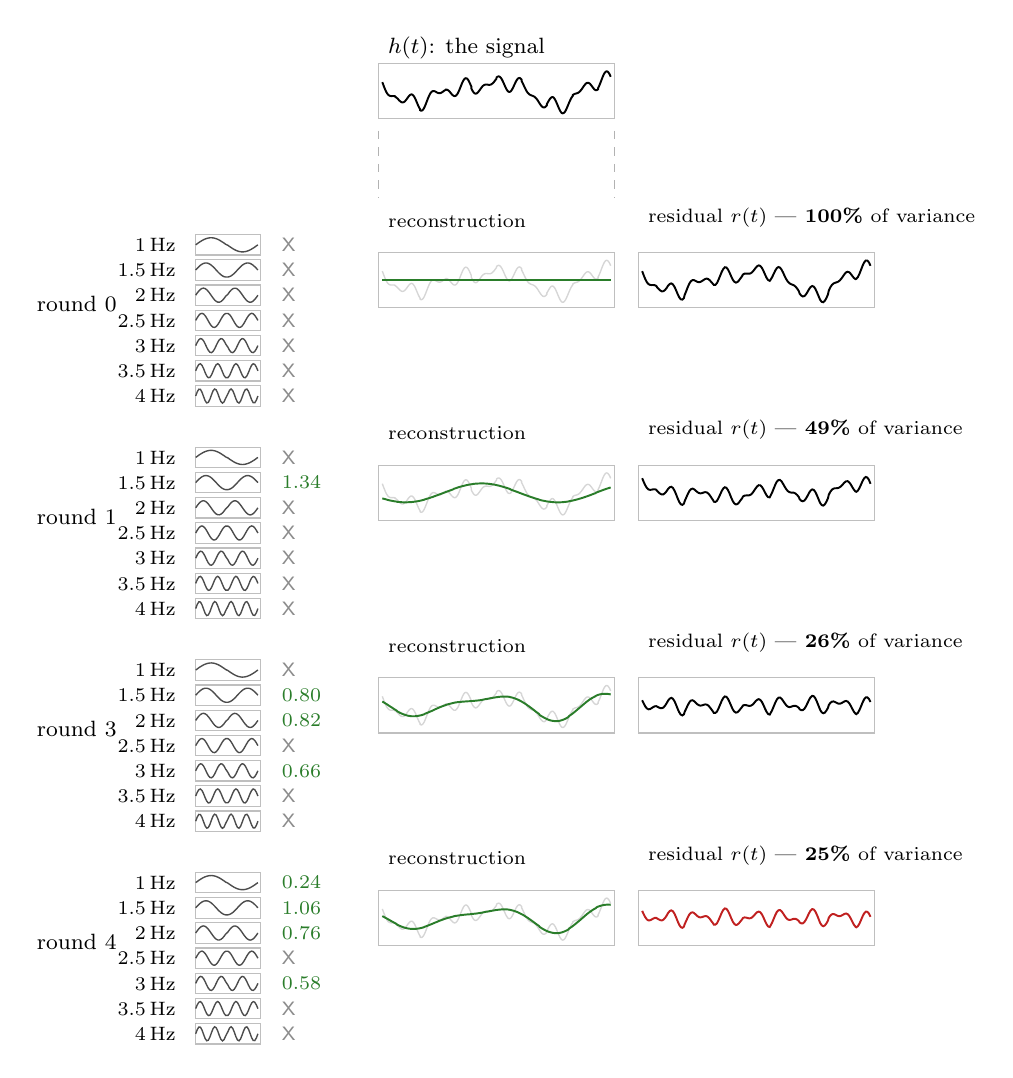
\begin{tikzpicture}[x=1cm,y=1cm,lab/.style={font=\footnotesize},lil/.style={font=\scriptsize},wv/.style={line width=.7pt},bx/.style={draw=black!25,line width=.4pt}]
% ghost h(t): the true signal shifted into the reconstruction cell (y-1.7), drawn faint behind
% each round's green reconstruction so the convergence toward h is visible round by round.
\def\hghost{%
(2.95,-0.684) (2.96,-0.711) (2.97,-0.738) (2.98,-0.763) (2.99,-0.787) (3.00,-0.808) (3.01,-0.825) (3.02,-0.839) (3.03,-0.849) (3.04,-0.855)
(3.05,-0.859) (3.06,-0.861) (3.07,-0.861) (3.08,-0.860) (3.09,-0.860) (3.10,-0.861) (3.11,-0.863) (3.11,-0.867) (3.12,-0.873) (3.13,-0.881)
(3.14,-0.890) (3.15,-0.900) (3.16,-0.911) (3.17,-0.921) (3.18,-0.930) (3.19,-0.937) (3.20,-0.941) (3.21,-0.941) (3.22,-0.939) (3.23,-0.933)
(3.24,-0.924) (3.25,-0.912) (3.26,-0.899) (3.27,-0.885) (3.28,-0.871) (3.29,-0.859) (3.30,-0.849) (3.31,-0.842) (3.32,-0.840) (3.33,-0.842)
(3.34,-0.850) (3.35,-0.862) (3.36,-0.878) (3.37,-0.898) (3.38,-0.921) (3.39,-0.945) (3.40,-0.969) (3.41,-0.992) (3.42,-1.012) (3.43,-1.028)
(3.43,-1.040) (3.44,-1.046) (3.45,-1.046) (3.46,-1.041) (3.47,-1.029) (3.48,-1.013) (3.49,-0.992) (3.50,-0.968) (3.51,-0.942) (3.52,-0.916)
(3.53,-0.890) (3.54,-0.866) (3.55,-0.845) (3.56,-0.827) (3.57,-0.813) (3.58,-0.804) (3.59,-0.798) (3.60,-0.797) (3.61,-0.798) (3.62,-0.802)
(3.63,-0.807) (3.64,-0.813) (3.65,-0.818) (3.66,-0.822) (3.67,-0.824) (3.68,-0.824) (3.69,-0.822) (3.70,-0.818) (3.71,-0.812) (3.72,-0.805)
(3.73,-0.797) (3.74,-0.790) (3.75,-0.785) (3.76,-0.781) (3.76,-0.779) (3.77,-0.780) (3.78,-0.784) (3.79,-0.791) (3.80,-0.800) (3.81,-0.811)
(3.82,-0.823) (3.83,-0.835) (3.84,-0.845) (3.85,-0.854) (3.86,-0.860) (3.87,-0.861) (3.88,-0.859) (3.89,-0.851) (3.90,-0.839) (3.91,-0.823)
(3.92,-0.802) (3.93,-0.779) (3.94,-0.754) (3.95,-0.729) (3.96,-0.704) (3.97,-0.681) (3.98,-0.662) (3.99,-0.647) (4.00,-0.638) (4.01,-0.634)
(4.02,-0.636) (4.03,-0.643) (4.04,-0.656) (4.05,-0.673) (4.06,-0.694) (4.07,-0.716) (4.08,-0.739) (4.08,-0.762) (4.09,-0.783) (4.10,-0.801)
(4.11,-0.815) (4.12,-0.825) (4.13,-0.830) (4.14,-0.830) (4.15,-0.826) (4.16,-0.818) (4.17,-0.807) (4.18,-0.794) (4.19,-0.780) (4.20,-0.766)
(4.21,-0.752) (4.22,-0.740) (4.23,-0.730) (4.24,-0.723) (4.25,-0.718) (4.26,-0.715) (4.27,-0.714) (4.28,-0.715) (4.29,-0.716) (4.30,-0.718)
(4.31,-0.718) (4.32,-0.717) (4.33,-0.714) (4.34,-0.708) (4.35,-0.700) (4.36,-0.690) (4.37,-0.679) (4.38,-0.666) (4.39,-0.652) (4.40,-0.639)
(4.40,-0.626) (4.41,-0.617) (4.42,-0.612) (4.43,-0.611) (4.44,-0.615) (4.45,-0.623) (4.46,-0.636) (4.47,-0.652) (4.48,-0.672) (4.49,-0.694)
(4.50,-0.717) (4.51,-0.740) (4.52,-0.761) (4.53,-0.779) (4.54,-0.794) (4.55,-0.804) (4.56,-0.808) (4.57,-0.807) (4.58,-0.801) (4.59,-0.789)
(4.60,-0.773) (4.61,-0.754) (4.62,-0.733) (4.63,-0.711) (4.64,-0.690) (4.65,-0.670) (4.66,-0.654) (4.67,-0.641) (4.68,-0.634) (4.69,-0.631)
(4.70,-0.634) (4.71,-0.642) (4.72,-0.655) (4.72,-0.671) (4.73,-0.691) (4.74,-0.712) (4.75,-0.734) (4.76,-0.755) (4.77,-0.775) (4.78,-0.794)
(4.79,-0.810) (4.80,-0.823) (4.81,-0.833) (4.82,-0.841) (4.83,-0.847) (4.84,-0.851) (4.85,-0.855) (4.86,-0.858) (4.87,-0.863) (4.88,-0.868)
(4.89,-0.876) (4.90,-0.886) (4.91,-0.897) (4.92,-0.911) (4.93,-0.926) (4.94,-0.942) (4.95,-0.958) (4.96,-0.973) (4.97,-0.986) (4.98,-0.996)
(4.99,-1.003) (5.00,-1.006) (5.01,-1.005) (5.02,-0.999) (5.03,-0.990) (5.04,-0.977) (5.04,-0.961) (5.05,-0.944) (5.06,-0.927) (5.07,-0.910)
(5.08,-0.895) (5.09,-0.883) (5.10,-0.876) (5.11,-0.873) (5.12,-0.876) (5.13,-0.886) (5.14,-0.899) (5.15,-0.917) (5.16,-0.939) (5.17,-0.962)
(5.18,-0.987) (5.19,-1.010) (5.20,-1.032) (5.21,-1.051) (5.22,-1.066) (5.23,-1.076) (5.24,-1.080) (5.25,-1.078) (5.26,-1.071) (5.27,-1.059)
(5.28,-1.042) (5.29,-1.021) (5.30,-0.998) (5.31,-0.974) (5.32,-0.950) (5.33,-0.927) (5.34,-0.905) (5.35,-0.886) (5.36,-0.870) (5.37,-0.857)
(5.37,-0.847) (5.38,-0.840) (5.39,-0.835) (5.40,-0.831) (5.41,-0.829) (5.42,-0.826) (5.43,-0.822) (5.44,-0.817) (5.45,-0.810) (5.46,-0.800)
(5.47,-0.789) (5.48,-0.777) (5.49,-0.762) (5.50,-0.748) (5.51,-0.733) (5.52,-0.720) (5.53,-0.708) (5.54,-0.699) (5.55,-0.694) (5.56,-0.692)
(5.57,-0.694) (5.58,-0.699) (5.59,-0.708) (5.60,-0.720) (5.61,-0.733) (5.62,-0.747) (5.63,-0.760) (5.64,-0.772) (5.65,-0.781) (5.66,-0.786)
(5.67,-0.787) (5.68,-0.782) (5.69,-0.773) (5.69,-0.759) (5.70,-0.740) (5.71,-0.717) (5.72,-0.692) (5.73,-0.666) (5.74,-0.639) (5.75,-0.614)
(5.76,-0.591) (5.77,-0.572) (5.78,-0.558) (5.79,-0.549) (5.80,-0.547) (5.81,-0.550) (5.82,-0.559) (5.83,-0.573) (5.84,-0.591) (5.85,-0.616)}
\node[lab,anchor=west] at (2.9,1.45){$h(t)$: the signal};
\draw[bx] (2.9,0.55) rectangle (5.9,1.25);
\draw[wv,black] plot coordinates {
(2.95,1.016) (2.96,0.989) (2.97,0.962) (2.98,0.937) (2.99,0.913) (3.00,0.892) (3.01,0.875) (3.02,0.861) (3.03,0.851) (3.04,0.845)
(3.05,0.841) (3.06,0.839) (3.07,0.839) (3.08,0.840) (3.09,0.840) (3.10,0.839) (3.11,0.837) (3.11,0.833) (3.12,0.827) (3.13,0.819)
(3.14,0.810) (3.15,0.800) (3.16,0.789) (3.17,0.779) (3.18,0.770) (3.19,0.763) (3.20,0.759) (3.21,0.759) (3.22,0.761) (3.23,0.767)
(3.24,0.776) (3.25,0.788) (3.26,0.801) (3.27,0.815) (3.28,0.829) (3.29,0.841) (3.30,0.851) (3.31,0.858) (3.32,0.860) (3.33,0.858)
(3.34,0.850) (3.35,0.838) (3.36,0.822) (3.37,0.802) (3.38,0.779) (3.39,0.755) (3.40,0.731) (3.41,0.708) (3.42,0.688) (3.43,0.672)
(3.43,0.660) (3.44,0.654) (3.45,0.654) (3.46,0.659) (3.47,0.671) (3.48,0.687) (3.49,0.708) (3.50,0.732) (3.51,0.758) (3.52,0.784)
(3.53,0.810) (3.54,0.834) (3.55,0.855) (3.56,0.873) (3.57,0.887) (3.58,0.896) (3.59,0.902) (3.60,0.903) (3.61,0.902) (3.62,0.898)
(3.63,0.893) (3.64,0.887) (3.65,0.882) (3.66,0.878) (3.67,0.876) (3.68,0.876) (3.69,0.878) (3.70,0.882) (3.71,0.888) (3.72,0.895)
(3.73,0.903) (3.74,0.910) (3.75,0.915) (3.76,0.919) (3.76,0.921) (3.77,0.920) (3.78,0.916) (3.79,0.909) (3.80,0.900) (3.81,0.889)
(3.82,0.877) (3.83,0.865) (3.84,0.855) (3.85,0.846) (3.86,0.840) (3.87,0.839) (3.88,0.841) (3.89,0.849) (3.90,0.861) (3.91,0.877)
(3.92,0.898) (3.93,0.921) (3.94,0.946) (3.95,0.971) (3.96,0.996) (3.97,1.019) (3.98,1.038) (3.99,1.053) (4.00,1.062) (4.01,1.066)
(4.02,1.064) (4.03,1.057) (4.04,1.044) (4.05,1.027) (4.06,1.006) (4.07,0.984) (4.08,0.961) (4.08,0.938) (4.09,0.917) (4.10,0.899)
(4.11,0.885) (4.12,0.875) (4.13,0.870) (4.14,0.870) (4.15,0.874) (4.16,0.882) (4.17,0.893) (4.18,0.906) (4.19,0.920) (4.20,0.934)
(4.21,0.948) (4.22,0.960) (4.23,0.970) (4.24,0.977) (4.25,0.982) (4.26,0.985) (4.27,0.986) (4.28,0.985) (4.29,0.984) (4.30,0.982)
(4.31,0.982) (4.32,0.983) (4.33,0.986) (4.34,0.992) (4.35,1.000) (4.36,1.010) (4.37,1.021) (4.38,1.034) (4.39,1.048) (4.40,1.061)
(4.40,1.074) (4.41,1.083) (4.42,1.088) (4.43,1.089) (4.44,1.085) (4.45,1.077) (4.46,1.064) (4.47,1.048) (4.48,1.028) (4.49,1.006)
(4.50,0.983) (4.51,0.960) (4.52,0.939) (4.53,0.921) (4.54,0.906) (4.55,0.896) (4.56,0.892) (4.57,0.893) (4.58,0.899) (4.59,0.911)
(4.60,0.927) (4.61,0.946) (4.62,0.967) (4.63,0.989) (4.64,1.010) (4.65,1.030) (4.66,1.046) (4.67,1.059) (4.68,1.066) (4.69,1.069)
(4.70,1.066) (4.71,1.058) (4.72,1.045) (4.72,1.029) (4.73,1.009) (4.74,0.988) (4.75,0.966) (4.76,0.945) (4.77,0.925) (4.78,0.906)
(4.79,0.890) (4.80,0.877) (4.81,0.867) (4.82,0.859) (4.83,0.853) (4.84,0.849) (4.85,0.845) (4.86,0.842) (4.87,0.837) (4.88,0.832)
(4.89,0.824) (4.90,0.814) (4.91,0.803) (4.92,0.789) (4.93,0.774) (4.94,0.758) (4.95,0.742) (4.96,0.727) (4.97,0.714) (4.98,0.704)
(4.99,0.697) (5.00,0.694) (5.01,0.695) (5.02,0.701) (5.03,0.710) (5.04,0.723) (5.04,0.739) (5.05,0.756) (5.06,0.773) (5.07,0.790)
(5.08,0.805) (5.09,0.817) (5.10,0.824) (5.11,0.827) (5.12,0.824) (5.13,0.814) (5.14,0.801) (5.15,0.783) (5.16,0.761) (5.17,0.738)
(5.18,0.713) (5.19,0.690) (5.20,0.668) (5.21,0.649) (5.22,0.634) (5.23,0.624) (5.24,0.620) (5.25,0.622) (5.26,0.629) (5.27,0.641)
(5.28,0.658) (5.29,0.679) (5.30,0.702) (5.31,0.726) (5.32,0.750) (5.33,0.773) (5.34,0.795) (5.35,0.814) (5.36,0.830) (5.37,0.843)
(5.37,0.853) (5.38,0.860) (5.39,0.865) (5.40,0.869) (5.41,0.871) (5.42,0.874) (5.43,0.878) (5.44,0.883) (5.45,0.890) (5.46,0.900)
(5.47,0.911) (5.48,0.923) (5.49,0.938) (5.50,0.952) (5.51,0.967) (5.52,0.980) (5.53,0.992) (5.54,1.001) (5.55,1.006) (5.56,1.008)
(5.57,1.006) (5.58,1.001) (5.59,0.992) (5.60,0.980) (5.61,0.967) (5.62,0.953) (5.63,0.940) (5.64,0.928) (5.65,0.919) (5.66,0.914)
(5.67,0.913) (5.68,0.918) (5.69,0.927) (5.69,0.941) (5.70,0.960) (5.71,0.983) (5.72,1.008) (5.73,1.034) (5.74,1.061) (5.75,1.086)
(5.76,1.109) (5.77,1.128) (5.78,1.142) (5.79,1.151) (5.80,1.153) (5.81,1.150) (5.82,1.141) (5.83,1.127) (5.84,1.109) (5.85,1.084)
};
\draw[black!30,dashed,line width=.4pt] (2.9,0.4)--(2.9,-0.45); \draw[black!30,dashed,line width=.4pt] (5.9,0.4)--(5.9,-0.45);
\begin{scope}[shift={(0,-0.7)}]
\node[lab,anchor=east] at (-0.3,-1.1){round 0};
\node[lil,anchor=east] at (0.45,-0.35){1\,Hz};
\draw[bx] (0.58,-0.48) rectangle (1.4,-0.22);
\draw[black!70,line width=.5pt] plot coordinates {
(0.58,-0.350) (0.60,-0.336) (0.62,-0.321) (0.64,-0.308) (0.66,-0.296) (0.68,-0.285) (0.70,-0.276) (0.72,-0.269) (0.74,-0.264) (0.76,-0.261) (0.78,-0.260) (0.80,-0.262)
(0.82,-0.266) (0.84,-0.272) (0.86,-0.280) (0.88,-0.290) (0.90,-0.302) (0.92,-0.315) (0.94,-0.328) (0.96,-0.343) (0.99,-0.357) (1.01,-0.372) (1.03,-0.385) (1.05,-0.398)
(1.07,-0.410) (1.09,-0.420) (1.11,-0.428) (1.13,-0.434) (1.15,-0.438) (1.17,-0.440) (1.19,-0.439) (1.21,-0.436) (1.23,-0.431) (1.25,-0.424) (1.27,-0.415) (1.29,-0.404)
(1.31,-0.392) (1.33,-0.379) (1.35,-0.364) (1.37,-0.350)
};
\node[lil,black!45,anchor=west] at (1.55,-0.35){\textsf{X}};
\node[lil,anchor=east] at (0.45,-0.67){1.5\,Hz};
\draw[bx] (0.58,-0.80) rectangle (1.4,-0.54);
\draw[black!70,line width=.5pt] plot coordinates {
(0.58,-0.670) (0.60,-0.648) (0.62,-0.628) (0.64,-0.610) (0.66,-0.596) (0.68,-0.586) (0.70,-0.581) (0.72,-0.581) (0.74,-0.586) (0.76,-0.596) (0.78,-0.610) (0.80,-0.628)
(0.82,-0.648) (0.84,-0.670) (0.86,-0.692) (0.88,-0.712) (0.90,-0.730) (0.92,-0.744) (0.94,-0.754) (0.96,-0.759) (0.99,-0.759) (1.01,-0.754) (1.03,-0.744) (1.05,-0.730)
(1.07,-0.712) (1.09,-0.692) (1.11,-0.670) (1.13,-0.648) (1.15,-0.628) (1.17,-0.610) (1.19,-0.596) (1.21,-0.586) (1.23,-0.581) (1.25,-0.581) (1.27,-0.586) (1.29,-0.596)
(1.31,-0.610) (1.33,-0.628) (1.35,-0.648) (1.37,-0.670)
};
\node[lil,black!45,anchor=west] at (1.55,-0.67){\textsf{X}};
\node[lil,anchor=east] at (0.45,-0.99){2\,Hz};
\draw[bx] (0.58,-1.12) rectangle (1.4,-0.86);
\draw[black!70,line width=.5pt] plot coordinates {
(0.58,-0.990) (0.60,-0.961) (0.62,-0.936) (0.64,-0.916) (0.66,-0.904) (0.68,-0.900) (0.70,-0.906) (0.72,-0.920) (0.74,-0.942) (0.76,-0.968) (0.78,-0.997) (0.80,-1.025)
(0.82,-1.050) (0.84,-1.068) (0.86,-1.078) (0.88,-1.079) (0.90,-1.071) (0.92,-1.055) (0.94,-1.032) (0.96,-1.004) (0.99,-0.976) (1.01,-0.948) (1.03,-0.925) (1.05,-0.909)
(1.07,-0.901) (1.09,-0.902) (1.11,-0.912) (1.13,-0.930) (1.15,-0.955) (1.17,-0.983) (1.19,-1.012) (1.21,-1.038) (1.23,-1.060) (1.25,-1.074) (1.27,-1.080) (1.29,-1.076)
(1.31,-1.064) (1.33,-1.044) (1.35,-1.019) (1.37,-0.990)
};
\node[lil,black!45,anchor=west] at (1.55,-0.99){\textsf{X}};
\node[lil,anchor=east] at (0.45,-1.31){2.5\,Hz};
\draw[bx] (0.58,-1.44) rectangle (1.4,-1.18);
\draw[black!70,line width=.5pt] plot coordinates {
(0.58,-1.310) (0.60,-1.275) (0.62,-1.245) (0.64,-1.226) (0.66,-1.220) (0.68,-1.229) (0.70,-1.250) (0.72,-1.281) (0.74,-1.317) (0.76,-1.352) (0.78,-1.380) (0.80,-1.396)
(0.82,-1.399) (0.84,-1.388) (0.86,-1.364) (0.88,-1.332) (0.90,-1.296) (0.92,-1.262) (0.94,-1.236) (0.96,-1.222) (0.99,-1.222) (1.01,-1.236) (1.03,-1.262) (1.05,-1.296)
(1.07,-1.332) (1.09,-1.364) (1.11,-1.388) (1.13,-1.399) (1.15,-1.396) (1.17,-1.380) (1.19,-1.352) (1.21,-1.317) (1.23,-1.281) (1.25,-1.250) (1.27,-1.229) (1.29,-1.220)
(1.31,-1.226) (1.33,-1.245) (1.35,-1.275) (1.37,-1.310)
};
\node[lil,black!45,anchor=west] at (1.55,-1.31){\textsf{X}};
\node[lil,anchor=east] at (0.45,-1.63){3\,Hz};
\draw[bx] (0.58,-1.76) rectangle (1.4,-1.50);
\draw[black!70,line width=.5pt] plot coordinates {
(0.58,-1.630) (0.60,-1.588) (0.62,-1.556) (0.64,-1.541) (0.66,-1.546) (0.68,-1.570) (0.70,-1.608) (0.72,-1.652) (0.74,-1.690) (0.76,-1.714) (0.78,-1.719) (0.80,-1.704)
(0.82,-1.672) (0.84,-1.630) (0.86,-1.588) (0.88,-1.556) (0.90,-1.541) (0.92,-1.546) (0.94,-1.570) (0.96,-1.608) (0.99,-1.652) (1.01,-1.690) (1.03,-1.714) (1.05,-1.719)
(1.07,-1.704) (1.09,-1.672) (1.11,-1.630) (1.13,-1.588) (1.15,-1.556) (1.17,-1.541) (1.19,-1.546) (1.21,-1.570) (1.23,-1.608) (1.25,-1.652) (1.27,-1.690) (1.29,-1.714)
(1.31,-1.719) (1.33,-1.704) (1.35,-1.672) (1.37,-1.630)
};
\node[lil,black!45,anchor=west] at (1.55,-1.63){\textsf{X}};
\node[lil,anchor=east] at (0.45,-1.95){3.5\,Hz};
\draw[bx] (0.58,-2.08) rectangle (1.4,-1.82);
\draw[black!70,line width=.5pt] plot coordinates {
(0.58,-1.950) (0.60,-1.902) (0.62,-1.869) (0.64,-1.861) (0.66,-1.880) (0.68,-1.921) (0.70,-1.972) (0.72,-2.015) (0.74,-2.038) (0.76,-2.034) (0.78,-2.004) (0.80,-1.957)
(0.82,-1.908) (0.84,-1.872) (0.86,-1.860) (0.88,-1.876) (0.90,-1.915) (0.92,-1.964) (0.94,-2.010) (0.96,-2.036) (0.99,-2.036) (1.01,-2.010) (1.03,-1.964) (1.05,-1.915)
(1.07,-1.876) (1.09,-1.860) (1.11,-1.872) (1.13,-1.908) (1.15,-1.957) (1.17,-2.004) (1.19,-2.034) (1.21,-2.038) (1.23,-2.015) (1.25,-1.972) (1.27,-1.921) (1.29,-1.880)
(1.31,-1.861) (1.33,-1.869) (1.35,-1.902) (1.37,-1.950)
};
\node[lil,black!45,anchor=west] at (1.55,-1.95){\textsf{X}};
\node[lil,anchor=east] at (0.45,-2.27){4\,Hz};
\draw[bx] (0.58,-2.40) rectangle (1.4,-2.14);
\draw[black!70,line width=.5pt] plot coordinates {
(0.58,-2.270) (0.60,-2.216) (0.62,-2.184) (0.64,-2.186) (0.66,-2.222) (0.68,-2.277) (0.70,-2.330) (0.72,-2.358) (0.74,-2.351) (0.76,-2.312) (0.78,-2.256) (0.80,-2.205)
(0.82,-2.181) (0.84,-2.192) (0.86,-2.235) (0.88,-2.292) (0.90,-2.340) (0.92,-2.360) (0.94,-2.344) (0.96,-2.299) (0.99,-2.241) (1.01,-2.196) (1.03,-2.180) (1.05,-2.200)
(1.07,-2.248) (1.09,-2.305) (1.11,-2.348) (1.13,-2.359) (1.15,-2.335) (1.17,-2.284) (1.19,-2.228) (1.21,-2.189) (1.23,-2.182) (1.25,-2.210) (1.27,-2.263) (1.29,-2.318)
(1.31,-2.354) (1.33,-2.356) (1.35,-2.324) (1.37,-2.270)
};
\node[lil,black!45,anchor=west] at (1.55,-2.27){\textsf{X}};
\node[lil,anchor=south west] at (2.9,-0.25){reconstruction};
\draw[bx] (2.9,-1.15) rectangle (5.9,-0.45);
\draw[black,opacity=0.16,line width=.5pt] plot coordinates {\hghost};
\draw[wv,fgrab] plot coordinates {
(2.95,-0.800) (2.97,-0.800) (2.99,-0.800) (3.01,-0.800) (3.03,-0.800) (3.05,-0.800) (3.07,-0.800) (3.09,-0.800) (3.11,-0.800) (3.13,-0.800)
(3.14,-0.800) (3.16,-0.800) (3.18,-0.800) (3.20,-0.800) (3.22,-0.800) (3.24,-0.800) (3.26,-0.800) (3.28,-0.800) (3.30,-0.800) (3.32,-0.800)
(3.34,-0.800) (3.36,-0.800) (3.38,-0.800) (3.40,-0.800) (3.42,-0.800) (3.44,-0.800) (3.46,-0.800) (3.48,-0.800) (3.49,-0.800) (3.51,-0.800)
(3.53,-0.800) (3.55,-0.800) (3.57,-0.800) (3.59,-0.800) (3.61,-0.800) (3.63,-0.800) (3.65,-0.800) (3.67,-0.800) (3.69,-0.800) (3.71,-0.800)
(3.73,-0.800) (3.75,-0.800) (3.77,-0.800) (3.79,-0.800) (3.81,-0.800) (3.83,-0.800) (3.85,-0.800) (3.86,-0.800) (3.88,-0.800) (3.90,-0.800)
(3.92,-0.800) (3.94,-0.800) (3.96,-0.800) (3.98,-0.800) (4.00,-0.800) (4.02,-0.800) (4.04,-0.800) (4.06,-0.800) (4.08,-0.800) (4.10,-0.800)
(4.12,-0.800) (4.14,-0.800) (4.16,-0.800) (4.18,-0.800) (4.20,-0.800) (4.22,-0.800) (4.23,-0.800) (4.25,-0.800) (4.27,-0.800) (4.29,-0.800)
(4.31,-0.800) (4.33,-0.800) (4.35,-0.800) (4.37,-0.800) (4.39,-0.800) (4.41,-0.800) (4.43,-0.800) (4.45,-0.800) (4.47,-0.800) (4.49,-0.800)
(4.51,-0.800) (4.53,-0.800) (4.55,-0.800) (4.57,-0.800) (4.58,-0.800) (4.60,-0.800) (4.62,-0.800) (4.64,-0.800) (4.66,-0.800) (4.68,-0.800)
(4.70,-0.800) (4.72,-0.800) (4.74,-0.800) (4.76,-0.800) (4.78,-0.800) (4.80,-0.800) (4.82,-0.800) (4.84,-0.800) (4.86,-0.800) (4.88,-0.800)
(4.90,-0.800) (4.92,-0.800) (4.94,-0.800) (4.95,-0.800) (4.97,-0.800) (4.99,-0.800) (5.01,-0.800) (5.03,-0.800) (5.05,-0.800) (5.07,-0.800)
(5.09,-0.800) (5.11,-0.800) (5.13,-0.800) (5.15,-0.800) (5.17,-0.800) (5.19,-0.800) (5.21,-0.800) (5.23,-0.800) (5.25,-0.800) (5.27,-0.800)
(5.29,-0.800) (5.31,-0.800) (5.32,-0.800) (5.34,-0.800) (5.36,-0.800) (5.38,-0.800) (5.40,-0.800) (5.42,-0.800) (5.44,-0.800) (5.46,-0.800)
(5.48,-0.800) (5.50,-0.800) (5.52,-0.800) (5.54,-0.800) (5.56,-0.800) (5.58,-0.800) (5.60,-0.800) (5.62,-0.800) (5.64,-0.800) (5.66,-0.800)
(5.67,-0.800) (5.69,-0.800) (5.71,-0.800) (5.73,-0.800) (5.75,-0.800) (5.77,-0.800) (5.79,-0.800) (5.81,-0.800) (5.83,-0.800) (5.85,-0.800)
};
\node[lil,anchor=south west] at (6.2,-0.25){residual $r(t)$ --- \textbf{100\%} of variance};
\draw[bx] (6.2,-1.15) rectangle (9.2,-0.45);
\draw[wv,black] plot coordinates {
(6.25,-0.684) (6.27,-0.738) (6.29,-0.787) (6.31,-0.825) (6.33,-0.849) (6.35,-0.859) (6.37,-0.861) (6.39,-0.860) (6.41,-0.863) (6.43,-0.873)
(6.44,-0.890) (6.46,-0.911) (6.48,-0.930) (6.50,-0.941) (6.52,-0.939) (6.54,-0.924) (6.56,-0.899) (6.58,-0.868) (6.60,-0.847) (6.62,-0.840)
(6.64,-0.852) (6.66,-0.882) (6.68,-0.925) (6.70,-0.974) (6.72,-1.016) (6.74,-1.042) (6.76,-1.046) (6.78,-1.026) (6.79,-0.987) (6.81,-0.937)
(6.83,-0.885) (6.85,-0.841) (6.87,-0.811) (6.89,-0.798) (6.91,-0.799) (6.93,-0.809) (6.95,-0.820) (6.97,-0.825) (6.99,-0.821) (7.01,-0.810)
(7.03,-0.796) (7.05,-0.784) (7.07,-0.779) (7.09,-0.785) (7.11,-0.802) (7.13,-0.825) (7.15,-0.847) (7.16,-0.860) (7.18,-0.858) (7.20,-0.836)
(7.22,-0.793) (7.24,-0.744) (7.26,-0.695) (7.28,-0.656) (7.30,-0.635) (7.32,-0.638) (7.34,-0.663) (7.36,-0.703) (7.38,-0.749) (7.40,-0.791)
(7.42,-0.819) (7.44,-0.830) (7.46,-0.823) (7.48,-0.802) (7.50,-0.774) (7.52,-0.747) (7.53,-0.727) (7.55,-0.716) (7.57,-0.715) (7.59,-0.717)
(7.61,-0.717) (7.63,-0.711) (7.65,-0.695) (7.67,-0.671) (7.69,-0.644) (7.71,-0.622) (7.73,-0.611) (7.75,-0.618) (7.77,-0.642) (7.79,-0.681)
(7.81,-0.726) (7.83,-0.769) (7.85,-0.798) (7.87,-0.808) (7.88,-0.794) (7.90,-0.762) (7.92,-0.720) (7.94,-0.678) (7.96,-0.646) (7.98,-0.632)
(8.00,-0.639) (8.02,-0.664) (8.04,-0.703) (8.06,-0.747) (8.08,-0.787) (8.10,-0.818) (8.12,-0.838) (8.14,-0.849) (8.16,-0.857) (8.18,-0.866)
(8.20,-0.883) (8.22,-0.908) (8.24,-0.939) (8.25,-0.970) (8.27,-0.994) (8.29,-1.006) (8.31,-1.001) (8.33,-0.980) (8.35,-0.948) (8.37,-0.913)
(8.39,-0.885) (8.41,-0.873) (8.43,-0.881) (8.45,-0.910) (8.47,-0.953) (8.49,-1.001) (8.51,-1.048) (8.53,-1.074) (8.55,-1.079) (8.57,-1.061)
(8.59,-1.026) (8.61,-0.979) (8.62,-0.931) (8.64,-0.890) (8.66,-0.859) (8.68,-0.841) (8.70,-0.832) (8.72,-0.826) (8.74,-0.818) (8.76,-0.802)
(8.78,-0.779) (8.80,-0.751) (8.82,-0.722) (8.84,-0.699) (8.86,-0.692) (8.88,-0.699) (8.90,-0.720) (8.92,-0.747) (8.94,-0.772) (8.96,-0.786)
(8.97,-0.782) (8.99,-0.759) (9.01,-0.717) (9.03,-0.666) (9.05,-0.614) (9.07,-0.572) (9.09,-0.549) (9.11,-0.550) (9.13,-0.573) (9.15,-0.616)
};
\end{scope}
\begin{scope}[shift={(0,-3.4000000000000004)}]
\node[lab,anchor=east] at (-0.3,-1.1){round 1};
\node[lil,anchor=east] at (0.45,-0.35){1\,Hz};
\draw[bx] (0.58,-0.48) rectangle (1.4,-0.22);
\draw[black!70,line width=.5pt] plot coordinates {
(0.58,-0.350) (0.60,-0.336) (0.62,-0.321) (0.64,-0.308) (0.66,-0.296) (0.68,-0.285) (0.70,-0.276) (0.72,-0.269) (0.74,-0.264) (0.76,-0.261) (0.78,-0.260) (0.80,-0.262)
(0.82,-0.266) (0.84,-0.272) (0.86,-0.280) (0.88,-0.290) (0.90,-0.302) (0.92,-0.315) (0.94,-0.328) (0.96,-0.343) (0.99,-0.357) (1.01,-0.372) (1.03,-0.385) (1.05,-0.398)
(1.07,-0.410) (1.09,-0.420) (1.11,-0.428) (1.13,-0.434) (1.15,-0.438) (1.17,-0.440) (1.19,-0.439) (1.21,-0.436) (1.23,-0.431) (1.25,-0.424) (1.27,-0.415) (1.29,-0.404)
(1.31,-0.392) (1.33,-0.379) (1.35,-0.364) (1.37,-0.350)
};
\node[lil,black!45,anchor=west] at (1.55,-0.35){\textsf{X}};
\node[lil,anchor=east] at (0.45,-0.67){1.5\,Hz};
\draw[bx] (0.58,-0.80) rectangle (1.4,-0.54);
\draw[black!70,line width=.5pt] plot coordinates {
(0.58,-0.670) (0.60,-0.648) (0.62,-0.628) (0.64,-0.610) (0.66,-0.596) (0.68,-0.586) (0.70,-0.581) (0.72,-0.581) (0.74,-0.586) (0.76,-0.596) (0.78,-0.610) (0.80,-0.628)
(0.82,-0.648) (0.84,-0.670) (0.86,-0.692) (0.88,-0.712) (0.90,-0.730) (0.92,-0.744) (0.94,-0.754) (0.96,-0.759) (0.99,-0.759) (1.01,-0.754) (1.03,-0.744) (1.05,-0.730)
(1.07,-0.712) (1.09,-0.692) (1.11,-0.670) (1.13,-0.648) (1.15,-0.628) (1.17,-0.610) (1.19,-0.596) (1.21,-0.586) (1.23,-0.581) (1.25,-0.581) (1.27,-0.586) (1.29,-0.596)
(1.31,-0.610) (1.33,-0.628) (1.35,-0.648) (1.37,-0.670)
};
\node[lil,fgrab,anchor=west] at (1.55,-0.67){1.34};
\node[lil,anchor=east] at (0.45,-0.99){2\,Hz};
\draw[bx] (0.58,-1.12) rectangle (1.4,-0.86);
\draw[black!70,line width=.5pt] plot coordinates {
(0.58,-0.990) (0.60,-0.961) (0.62,-0.936) (0.64,-0.916) (0.66,-0.904) (0.68,-0.900) (0.70,-0.906) (0.72,-0.920) (0.74,-0.942) (0.76,-0.968) (0.78,-0.997) (0.80,-1.025)
(0.82,-1.050) (0.84,-1.068) (0.86,-1.078) (0.88,-1.079) (0.90,-1.071) (0.92,-1.055) (0.94,-1.032) (0.96,-1.004) (0.99,-0.976) (1.01,-0.948) (1.03,-0.925) (1.05,-0.909)
(1.07,-0.901) (1.09,-0.902) (1.11,-0.912) (1.13,-0.930) (1.15,-0.955) (1.17,-0.983) (1.19,-1.012) (1.21,-1.038) (1.23,-1.060) (1.25,-1.074) (1.27,-1.080) (1.29,-1.076)
(1.31,-1.064) (1.33,-1.044) (1.35,-1.019) (1.37,-0.990)
};
\node[lil,black!45,anchor=west] at (1.55,-0.99){\textsf{X}};
\node[lil,anchor=east] at (0.45,-1.31){2.5\,Hz};
\draw[bx] (0.58,-1.44) rectangle (1.4,-1.18);
\draw[black!70,line width=.5pt] plot coordinates {
(0.58,-1.310) (0.60,-1.275) (0.62,-1.245) (0.64,-1.226) (0.66,-1.220) (0.68,-1.229) (0.70,-1.250) (0.72,-1.281) (0.74,-1.317) (0.76,-1.352) (0.78,-1.380) (0.80,-1.396)
(0.82,-1.399) (0.84,-1.388) (0.86,-1.364) (0.88,-1.332) (0.90,-1.296) (0.92,-1.262) (0.94,-1.236) (0.96,-1.222) (0.99,-1.222) (1.01,-1.236) (1.03,-1.262) (1.05,-1.296)
(1.07,-1.332) (1.09,-1.364) (1.11,-1.388) (1.13,-1.399) (1.15,-1.396) (1.17,-1.380) (1.19,-1.352) (1.21,-1.317) (1.23,-1.281) (1.25,-1.250) (1.27,-1.229) (1.29,-1.220)
(1.31,-1.226) (1.33,-1.245) (1.35,-1.275) (1.37,-1.310)
};
\node[lil,black!45,anchor=west] at (1.55,-1.31){\textsf{X}};
\node[lil,anchor=east] at (0.45,-1.63){3\,Hz};
\draw[bx] (0.58,-1.76) rectangle (1.4,-1.50);
\draw[black!70,line width=.5pt] plot coordinates {
(0.58,-1.630) (0.60,-1.588) (0.62,-1.556) (0.64,-1.541) (0.66,-1.546) (0.68,-1.570) (0.70,-1.608) (0.72,-1.652) (0.74,-1.690) (0.76,-1.714) (0.78,-1.719) (0.80,-1.704)
(0.82,-1.672) (0.84,-1.630) (0.86,-1.588) (0.88,-1.556) (0.90,-1.541) (0.92,-1.546) (0.94,-1.570) (0.96,-1.608) (0.99,-1.652) (1.01,-1.690) (1.03,-1.714) (1.05,-1.719)
(1.07,-1.704) (1.09,-1.672) (1.11,-1.630) (1.13,-1.588) (1.15,-1.556) (1.17,-1.541) (1.19,-1.546) (1.21,-1.570) (1.23,-1.608) (1.25,-1.652) (1.27,-1.690) (1.29,-1.714)
(1.31,-1.719) (1.33,-1.704) (1.35,-1.672) (1.37,-1.630)
};
\node[lil,black!45,anchor=west] at (1.55,-1.63){\textsf{X}};
\node[lil,anchor=east] at (0.45,-1.95){3.5\,Hz};
\draw[bx] (0.58,-2.08) rectangle (1.4,-1.82);
\draw[black!70,line width=.5pt] plot coordinates {
(0.58,-1.950) (0.60,-1.902) (0.62,-1.869) (0.64,-1.861) (0.66,-1.880) (0.68,-1.921) (0.70,-1.972) (0.72,-2.015) (0.74,-2.038) (0.76,-2.034) (0.78,-2.004) (0.80,-1.957)
(0.82,-1.908) (0.84,-1.872) (0.86,-1.860) (0.88,-1.876) (0.90,-1.915) (0.92,-1.964) (0.94,-2.010) (0.96,-2.036) (0.99,-2.036) (1.01,-2.010) (1.03,-1.964) (1.05,-1.915)
(1.07,-1.876) (1.09,-1.860) (1.11,-1.872) (1.13,-1.908) (1.15,-1.957) (1.17,-2.004) (1.19,-2.034) (1.21,-2.038) (1.23,-2.015) (1.25,-1.972) (1.27,-1.921) (1.29,-1.880)
(1.31,-1.861) (1.33,-1.869) (1.35,-1.902) (1.37,-1.950)
};
\node[lil,black!45,anchor=west] at (1.55,-1.95){\textsf{X}};
\node[lil,anchor=east] at (0.45,-2.27){4\,Hz};
\draw[bx] (0.58,-2.40) rectangle (1.4,-2.14);
\draw[black!70,line width=.5pt] plot coordinates {
(0.58,-2.270) (0.60,-2.216) (0.62,-2.184) (0.64,-2.186) (0.66,-2.222) (0.68,-2.277) (0.70,-2.330) (0.72,-2.358) (0.74,-2.351) (0.76,-2.312) (0.78,-2.256) (0.80,-2.205)
(0.82,-2.181) (0.84,-2.192) (0.86,-2.235) (0.88,-2.292) (0.90,-2.340) (0.92,-2.360) (0.94,-2.344) (0.96,-2.299) (0.99,-2.241) (1.01,-2.196) (1.03,-2.180) (1.05,-2.200)
(1.07,-2.248) (1.09,-2.305) (1.11,-2.348) (1.13,-2.359) (1.15,-2.335) (1.17,-2.284) (1.19,-2.228) (1.21,-2.189) (1.23,-2.182) (1.25,-2.210) (1.27,-2.263) (1.29,-2.318)
(1.31,-2.354) (1.33,-2.356) (1.35,-2.324) (1.37,-2.270)
};
\node[lil,black!45,anchor=west] at (1.55,-2.27){\textsf{X}};
\node[lil,anchor=south west] at (2.9,-0.25){reconstruction};
\draw[bx] (2.9,-1.15) rectangle (5.9,-0.45);
\draw[black,opacity=0.16,line width=.5pt] plot coordinates {\hghost};
\draw[wv,fgrab] plot coordinates {
(2.95,-0.870) (2.97,-0.876) (2.99,-0.881) (3.01,-0.887) (3.03,-0.892) (3.05,-0.897) (3.07,-0.901) (3.09,-0.905) (3.11,-0.908) (3.13,-0.911)
(3.14,-0.914) (3.16,-0.916) (3.18,-0.918) (3.20,-0.919) (3.22,-0.920) (3.24,-0.920) (3.26,-0.920) (3.28,-0.919) (3.30,-0.918) (3.32,-0.917)
(3.34,-0.915) (3.36,-0.912) (3.38,-0.909) (3.40,-0.906) (3.42,-0.902) (3.44,-0.898) (3.46,-0.893) (3.48,-0.888) (3.49,-0.883) (3.51,-0.877)
(3.53,-0.871) (3.55,-0.865) (3.57,-0.858) (3.59,-0.852) (3.61,-0.844) (3.63,-0.837) (3.65,-0.830) (3.67,-0.822) (3.69,-0.815) (3.71,-0.807)
(3.73,-0.800) (3.75,-0.792) (3.77,-0.785) (3.79,-0.777) (3.81,-0.770) (3.83,-0.763) (3.85,-0.755) (3.86,-0.748) (3.88,-0.742) (3.90,-0.735)
(3.92,-0.728) (3.94,-0.722) (3.96,-0.717) (3.98,-0.712) (4.00,-0.707) (4.02,-0.702) (4.04,-0.698) (4.06,-0.694) (4.08,-0.691) (4.10,-0.688)
(4.12,-0.685) (4.14,-0.683) (4.16,-0.682) (4.18,-0.681) (4.20,-0.680) (4.22,-0.680) (4.23,-0.680) (4.25,-0.681) (4.27,-0.682) (4.29,-0.684)
(4.31,-0.686) (4.33,-0.689) (4.35,-0.692) (4.37,-0.695) (4.39,-0.699) (4.41,-0.704) (4.43,-0.708) (4.45,-0.714) (4.47,-0.719) (4.49,-0.725)
(4.51,-0.731) (4.53,-0.737) (4.55,-0.744) (4.57,-0.751) (4.58,-0.758) (4.60,-0.765) (4.62,-0.773) (4.64,-0.780) (4.66,-0.787) (4.68,-0.795)
(4.70,-0.803) (4.72,-0.810) (4.74,-0.818) (4.76,-0.825) (4.78,-0.832) (4.80,-0.840) (4.82,-0.847) (4.84,-0.854) (4.86,-0.860) (4.88,-0.867)
(4.90,-0.873) (4.92,-0.879) (4.94,-0.885) (4.95,-0.890) (4.97,-0.895) (4.99,-0.899) (5.01,-0.903) (5.03,-0.907) (5.05,-0.910) (5.07,-0.913)
(5.09,-0.915) (5.11,-0.917) (5.13,-0.919) (5.15,-0.920) (5.17,-0.920) (5.19,-0.920) (5.21,-0.920) (5.23,-0.919) (5.25,-0.917) (5.27,-0.915)
(5.29,-0.913) (5.31,-0.910) (5.32,-0.907) (5.34,-0.903) (5.36,-0.899) (5.38,-0.895) (5.40,-0.890) (5.42,-0.885) (5.44,-0.879) (5.46,-0.873)
(5.48,-0.867) (5.50,-0.861) (5.52,-0.854) (5.54,-0.847) (5.56,-0.840) (5.58,-0.833) (5.60,-0.825) (5.62,-0.818) (5.64,-0.810) (5.66,-0.803)
(5.67,-0.795) (5.69,-0.788) (5.71,-0.780) (5.73,-0.773) (5.75,-0.765) (5.77,-0.758) (5.79,-0.751) (5.81,-0.744) (5.83,-0.738) (5.85,-0.731)
};
\node[lil,anchor=south west] at (6.2,-0.25){residual $r(t)$ --- \textbf{49\%} of variance};
\draw[bx] (6.2,-1.15) rectangle (9.2,-0.45);
\draw[wv,black] plot coordinates {
(6.25,-0.614) (6.27,-0.662) (6.29,-0.705) (6.31,-0.738) (6.33,-0.757) (6.35,-0.762) (6.37,-0.760) (6.39,-0.755) (6.41,-0.754) (6.43,-0.761)
(6.44,-0.776) (6.46,-0.795) (6.48,-0.812) (6.50,-0.821) (6.52,-0.819) (6.54,-0.803) (6.56,-0.779) (6.58,-0.749) (6.60,-0.729) (6.62,-0.723)
(6.64,-0.737) (6.66,-0.770) (6.68,-0.816) (6.70,-0.868) (6.72,-0.914) (6.74,-0.944) (6.76,-0.953) (6.78,-0.938) (6.79,-0.905) (6.81,-0.860)
(6.83,-0.814) (6.85,-0.776) (6.87,-0.753) (6.89,-0.746) (6.91,-0.755) (6.93,-0.772) (6.95,-0.790) (6.97,-0.802) (6.99,-0.807) (7.01,-0.803)
(7.03,-0.796) (7.05,-0.791) (7.07,-0.794) (7.09,-0.808) (7.11,-0.832) (7.13,-0.863) (7.15,-0.892) (7.16,-0.912) (7.18,-0.916) (7.20,-0.901)
(7.22,-0.865) (7.24,-0.822) (7.26,-0.778) (7.28,-0.744) (7.30,-0.729) (7.32,-0.736) (7.34,-0.765) (7.36,-0.808) (7.38,-0.858) (7.40,-0.903)
(7.42,-0.934) (7.44,-0.947) (7.46,-0.942) (7.48,-0.922) (7.50,-0.894) (7.52,-0.868) (7.53,-0.847) (7.55,-0.835) (7.57,-0.833) (7.59,-0.833)
(7.61,-0.831) (7.63,-0.822) (7.65,-0.803) (7.67,-0.775) (7.69,-0.745) (7.71,-0.718) (7.73,-0.703) (7.75,-0.704) (7.77,-0.723) (7.79,-0.756)
(7.81,-0.795) (7.83,-0.832) (7.85,-0.855) (7.87,-0.857) (7.88,-0.836) (7.90,-0.797) (7.92,-0.747) (7.94,-0.698) (7.96,-0.658) (7.98,-0.637)
(8.00,-0.636) (8.02,-0.654) (8.04,-0.686) (8.06,-0.722) (8.08,-0.754) (8.10,-0.778) (8.12,-0.791) (8.14,-0.796) (8.16,-0.796) (8.18,-0.799)
(8.20,-0.810) (8.22,-0.829) (8.24,-0.854) (8.25,-0.880) (8.27,-0.900) (8.29,-0.907) (8.31,-0.898) (8.33,-0.873) (8.35,-0.838) (8.37,-0.800)
(8.39,-0.770) (8.41,-0.756) (8.43,-0.763) (8.45,-0.790) (8.47,-0.832) (8.49,-0.881) (8.51,-0.928) (8.53,-0.955) (8.55,-0.962) (8.57,-0.946)
(8.59,-0.912) (8.61,-0.869) (8.62,-0.824) (8.64,-0.786) (8.66,-0.760) (8.68,-0.746) (8.70,-0.742) (8.72,-0.741) (8.74,-0.738) (8.76,-0.729)
(8.78,-0.712) (8.80,-0.690) (8.82,-0.668) (8.84,-0.653) (8.86,-0.652) (8.88,-0.667) (8.90,-0.694) (8.92,-0.729) (8.94,-0.761) (8.96,-0.783)
(8.97,-0.787) (8.99,-0.771) (9.01,-0.737) (9.03,-0.693) (9.05,-0.648) (9.07,-0.614) (9.09,-0.598) (9.11,-0.606) (9.13,-0.635) (9.15,-0.685)
};
\end{scope}
\begin{scope}[shift={(0,-6.1000000000000005)}]
\node[lab,anchor=east] at (-0.3,-1.1){round 3};
\node[lil,anchor=east] at (0.45,-0.35){1\,Hz};
\draw[bx] (0.58,-0.48) rectangle (1.4,-0.22);
\draw[black!70,line width=.5pt] plot coordinates {
(0.58,-0.350) (0.60,-0.336) (0.62,-0.321) (0.64,-0.308) (0.66,-0.296) (0.68,-0.285) (0.70,-0.276) (0.72,-0.269) (0.74,-0.264) (0.76,-0.261) (0.78,-0.260) (0.80,-0.262)
(0.82,-0.266) (0.84,-0.272) (0.86,-0.280) (0.88,-0.290) (0.90,-0.302) (0.92,-0.315) (0.94,-0.328) (0.96,-0.343) (0.99,-0.357) (1.01,-0.372) (1.03,-0.385) (1.05,-0.398)
(1.07,-0.410) (1.09,-0.420) (1.11,-0.428) (1.13,-0.434) (1.15,-0.438) (1.17,-0.440) (1.19,-0.439) (1.21,-0.436) (1.23,-0.431) (1.25,-0.424) (1.27,-0.415) (1.29,-0.404)
(1.31,-0.392) (1.33,-0.379) (1.35,-0.364) (1.37,-0.350)
};
\node[lil,black!45,anchor=west] at (1.55,-0.35){\textsf{X}};
\node[lil,anchor=east] at (0.45,-0.67){1.5\,Hz};
\draw[bx] (0.58,-0.80) rectangle (1.4,-0.54);
\draw[black!70,line width=.5pt] plot coordinates {
(0.58,-0.670) (0.60,-0.648) (0.62,-0.628) (0.64,-0.610) (0.66,-0.596) (0.68,-0.586) (0.70,-0.581) (0.72,-0.581) (0.74,-0.586) (0.76,-0.596) (0.78,-0.610) (0.80,-0.628)
(0.82,-0.648) (0.84,-0.670) (0.86,-0.692) (0.88,-0.712) (0.90,-0.730) (0.92,-0.744) (0.94,-0.754) (0.96,-0.759) (0.99,-0.759) (1.01,-0.754) (1.03,-0.744) (1.05,-0.730)
(1.07,-0.712) (1.09,-0.692) (1.11,-0.670) (1.13,-0.648) (1.15,-0.628) (1.17,-0.610) (1.19,-0.596) (1.21,-0.586) (1.23,-0.581) (1.25,-0.581) (1.27,-0.586) (1.29,-0.596)
(1.31,-0.610) (1.33,-0.628) (1.35,-0.648) (1.37,-0.670)
};
\node[lil,fgrab,anchor=west] at (1.55,-0.67){0.80};
\node[lil,anchor=east] at (0.45,-0.99){2\,Hz};
\draw[bx] (0.58,-1.12) rectangle (1.4,-0.86);
\draw[black!70,line width=.5pt] plot coordinates {
(0.58,-0.990) (0.60,-0.961) (0.62,-0.936) (0.64,-0.916) (0.66,-0.904) (0.68,-0.900) (0.70,-0.906) (0.72,-0.920) (0.74,-0.942) (0.76,-0.968) (0.78,-0.997) (0.80,-1.025)
(0.82,-1.050) (0.84,-1.068) (0.86,-1.078) (0.88,-1.079) (0.90,-1.071) (0.92,-1.055) (0.94,-1.032) (0.96,-1.004) (0.99,-0.976) (1.01,-0.948) (1.03,-0.925) (1.05,-0.909)
(1.07,-0.901) (1.09,-0.902) (1.11,-0.912) (1.13,-0.930) (1.15,-0.955) (1.17,-0.983) (1.19,-1.012) (1.21,-1.038) (1.23,-1.060) (1.25,-1.074) (1.27,-1.080) (1.29,-1.076)
(1.31,-1.064) (1.33,-1.044) (1.35,-1.019) (1.37,-0.990)
};
\node[lil,fgrab,anchor=west] at (1.55,-0.99){0.82};
\node[lil,anchor=east] at (0.45,-1.31){2.5\,Hz};
\draw[bx] (0.58,-1.44) rectangle (1.4,-1.18);
\draw[black!70,line width=.5pt] plot coordinates {
(0.58,-1.310) (0.60,-1.275) (0.62,-1.245) (0.64,-1.226) (0.66,-1.220) (0.68,-1.229) (0.70,-1.250) (0.72,-1.281) (0.74,-1.317) (0.76,-1.352) (0.78,-1.380) (0.80,-1.396)
(0.82,-1.399) (0.84,-1.388) (0.86,-1.364) (0.88,-1.332) (0.90,-1.296) (0.92,-1.262) (0.94,-1.236) (0.96,-1.222) (0.99,-1.222) (1.01,-1.236) (1.03,-1.262) (1.05,-1.296)
(1.07,-1.332) (1.09,-1.364) (1.11,-1.388) (1.13,-1.399) (1.15,-1.396) (1.17,-1.380) (1.19,-1.352) (1.21,-1.317) (1.23,-1.281) (1.25,-1.250) (1.27,-1.229) (1.29,-1.220)
(1.31,-1.226) (1.33,-1.245) (1.35,-1.275) (1.37,-1.310)
};
\node[lil,black!45,anchor=west] at (1.55,-1.31){\textsf{X}};
\node[lil,anchor=east] at (0.45,-1.63){3\,Hz};
\draw[bx] (0.58,-1.76) rectangle (1.4,-1.50);
\draw[black!70,line width=.5pt] plot coordinates {
(0.58,-1.630) (0.60,-1.588) (0.62,-1.556) (0.64,-1.541) (0.66,-1.546) (0.68,-1.570) (0.70,-1.608) (0.72,-1.652) (0.74,-1.690) (0.76,-1.714) (0.78,-1.719) (0.80,-1.704)
(0.82,-1.672) (0.84,-1.630) (0.86,-1.588) (0.88,-1.556) (0.90,-1.541) (0.92,-1.546) (0.94,-1.570) (0.96,-1.608) (0.99,-1.652) (1.01,-1.690) (1.03,-1.714) (1.05,-1.719)
(1.07,-1.704) (1.09,-1.672) (1.11,-1.630) (1.13,-1.588) (1.15,-1.556) (1.17,-1.541) (1.19,-1.546) (1.21,-1.570) (1.23,-1.608) (1.25,-1.652) (1.27,-1.690) (1.29,-1.714)
(1.31,-1.719) (1.33,-1.704) (1.35,-1.672) (1.37,-1.630)
};
\node[lil,fgrab,anchor=west] at (1.55,-1.63){0.66};
\node[lil,anchor=east] at (0.45,-1.95){3.5\,Hz};
\draw[bx] (0.58,-2.08) rectangle (1.4,-1.82);
\draw[black!70,line width=.5pt] plot coordinates {
(0.58,-1.950) (0.60,-1.902) (0.62,-1.869) (0.64,-1.861) (0.66,-1.880) (0.68,-1.921) (0.70,-1.972) (0.72,-2.015) (0.74,-2.038) (0.76,-2.034) (0.78,-2.004) (0.80,-1.957)
(0.82,-1.908) (0.84,-1.872) (0.86,-1.860) (0.88,-1.876) (0.90,-1.915) (0.92,-1.964) (0.94,-2.010) (0.96,-2.036) (0.99,-2.036) (1.01,-2.010) (1.03,-1.964) (1.05,-1.915)
(1.07,-1.876) (1.09,-1.860) (1.11,-1.872) (1.13,-1.908) (1.15,-1.957) (1.17,-2.004) (1.19,-2.034) (1.21,-2.038) (1.23,-2.015) (1.25,-1.972) (1.27,-1.921) (1.29,-1.880)
(1.31,-1.861) (1.33,-1.869) (1.35,-1.902) (1.37,-1.950)
};
\node[lil,black!45,anchor=west] at (1.55,-1.95){\textsf{X}};
\node[lil,anchor=east] at (0.45,-2.27){4\,Hz};
\draw[bx] (0.58,-2.40) rectangle (1.4,-2.14);
\draw[black!70,line width=.5pt] plot coordinates {
(0.58,-2.270) (0.60,-2.216) (0.62,-2.184) (0.64,-2.186) (0.66,-2.222) (0.68,-2.277) (0.70,-2.330) (0.72,-2.358) (0.74,-2.351) (0.76,-2.312) (0.78,-2.256) (0.80,-2.205)
(0.82,-2.181) (0.84,-2.192) (0.86,-2.235) (0.88,-2.292) (0.90,-2.340) (0.92,-2.360) (0.94,-2.344) (0.96,-2.299) (0.99,-2.241) (1.01,-2.196) (1.03,-2.180) (1.05,-2.200)
(1.07,-2.248) (1.09,-2.305) (1.11,-2.348) (1.13,-2.359) (1.15,-2.335) (1.17,-2.284) (1.19,-2.228) (1.21,-2.189) (1.23,-2.182) (1.25,-2.210) (1.27,-2.263) (1.29,-2.318)
(1.31,-2.354) (1.33,-2.356) (1.35,-2.324) (1.37,-2.270)
};
\node[lil,black!45,anchor=west] at (1.55,-2.27){\textsf{X}};
\node[lil,anchor=south west] at (2.9,-0.25){reconstruction};
\draw[bx] (2.9,-1.15) rectangle (5.9,-0.45);
\draw[black,opacity=0.16,line width=.5pt] plot coordinates {\hghost};
\draw[wv,fgrab] plot coordinates {
(2.95,-0.750) (2.97,-0.762) (2.99,-0.774) (3.01,-0.787) (3.03,-0.800) (3.05,-0.813) (3.07,-0.826) (3.09,-0.839) (3.11,-0.852) (3.13,-0.864)
(3.14,-0.875) (3.16,-0.886) (3.18,-0.896) (3.20,-0.905) (3.22,-0.913) (3.24,-0.920) (3.26,-0.926) (3.28,-0.931) (3.30,-0.934) (3.32,-0.937)
(3.34,-0.937) (3.36,-0.937) (3.38,-0.936) (3.40,-0.933) (3.42,-0.929) (3.44,-0.925) (3.46,-0.919) (3.48,-0.913) (3.49,-0.906) (3.51,-0.898)
(3.53,-0.890) (3.55,-0.881) (3.57,-0.873) (3.59,-0.864) (3.61,-0.854) (3.63,-0.845) (3.65,-0.836) (3.67,-0.827) (3.69,-0.819) (3.71,-0.811)
(3.73,-0.804) (3.75,-0.797) (3.77,-0.790) (3.79,-0.784) (3.81,-0.779) (3.83,-0.774) (3.85,-0.769) (3.86,-0.766) (3.88,-0.762) (3.90,-0.759)
(3.92,-0.757) (3.94,-0.755) (3.96,-0.753) (3.98,-0.751) (4.00,-0.750) (4.02,-0.748) (4.04,-0.747) (4.06,-0.746) (4.08,-0.744) (4.10,-0.743)
(4.12,-0.741) (4.14,-0.739) (4.16,-0.737) (4.18,-0.735) (4.20,-0.732) (4.22,-0.729) (4.23,-0.726) (4.25,-0.722) (4.27,-0.719) (4.29,-0.715)
(4.31,-0.711) (4.33,-0.707) (4.35,-0.704) (4.37,-0.700) (4.39,-0.697) (4.41,-0.694) (4.43,-0.691) (4.45,-0.689) (4.47,-0.688) (4.49,-0.687)
(4.51,-0.687) (4.53,-0.687) (4.55,-0.689) (4.57,-0.692) (4.58,-0.696) (4.60,-0.700) (4.62,-0.706) (4.64,-0.713) (4.66,-0.721) (4.68,-0.730)
(4.70,-0.740) (4.72,-0.751) (4.74,-0.763) (4.76,-0.775) (4.78,-0.789) (4.80,-0.803) (4.82,-0.817) (4.84,-0.832) (4.86,-0.847) (4.88,-0.862)
(4.90,-0.879) (4.92,-0.893) (4.94,-0.908) (4.95,-0.922) (4.97,-0.935) (4.99,-0.947) (5.01,-0.958) (5.03,-0.968) (5.05,-0.977) (5.07,-0.985)
(5.09,-0.991) (5.11,-0.995) (5.13,-0.998) (5.15,-0.999) (5.17,-0.999) (5.19,-0.997) (5.21,-0.993) (5.23,-0.987) (5.25,-0.980) (5.27,-0.971)
(5.29,-0.961) (5.31,-0.949) (5.32,-0.936) (5.34,-0.922) (5.36,-0.908) (5.38,-0.892) (5.40,-0.876) (5.42,-0.859) (5.44,-0.842) (5.46,-0.825)
(5.48,-0.808) (5.50,-0.791) (5.52,-0.774) (5.54,-0.757) (5.56,-0.742) (5.58,-0.727) (5.60,-0.714) (5.62,-0.702) (5.64,-0.691) (5.66,-0.681)
(5.67,-0.673) (5.69,-0.666) (5.71,-0.660) (5.73,-0.656) (5.75,-0.653) (5.77,-0.652) (5.79,-0.652) (5.81,-0.653) (5.83,-0.656) (5.85,-0.660)
};
\node[lil,anchor=south west] at (6.2,-0.25){residual $r(t)$ --- \textbf{26\%} of variance};
\draw[bx] (6.2,-1.15) rectangle (9.2,-0.45);
\draw[wv,black] plot coordinates {
(6.25,-0.734) (6.27,-0.775) (6.29,-0.813) (6.31,-0.838) (6.33,-0.849) (6.35,-0.846) (6.37,-0.834) (6.39,-0.821) (6.41,-0.811) (6.43,-0.809)
(6.44,-0.815) (6.46,-0.825) (6.48,-0.834) (6.50,-0.835) (6.52,-0.826) (6.54,-0.804) (6.56,-0.773) (6.58,-0.737) (6.60,-0.713) (6.62,-0.703)
(6.64,-0.714) (6.66,-0.745) (6.68,-0.790) (6.70,-0.841) (6.72,-0.886) (6.74,-0.917) (6.76,-0.927) (6.78,-0.913) (6.79,-0.881) (6.81,-0.839)
(6.83,-0.795) (6.85,-0.759) (6.87,-0.738) (6.89,-0.734) (6.91,-0.746) (6.93,-0.764) (6.95,-0.784) (6.97,-0.797) (6.99,-0.802) (7.01,-0.799)
(7.03,-0.792) (7.05,-0.787) (7.07,-0.789) (7.09,-0.801) (7.11,-0.824) (7.13,-0.851) (7.15,-0.878) (7.16,-0.895) (7.18,-0.895) (7.20,-0.877)
(7.22,-0.837) (7.24,-0.790) (7.26,-0.742) (7.28,-0.705) (7.30,-0.686) (7.32,-0.690) (7.34,-0.716) (7.36,-0.757) (7.38,-0.804) (7.40,-0.848)
(7.42,-0.878) (7.44,-0.891) (7.46,-0.886) (7.48,-0.868) (7.50,-0.842) (7.52,-0.818) (7.53,-0.801) (7.55,-0.794) (7.57,-0.796) (7.59,-0.802)
(7.61,-0.806) (7.63,-0.803) (7.65,-0.791) (7.67,-0.771) (7.69,-0.747) (7.71,-0.728) (7.73,-0.720) (7.75,-0.729) (7.77,-0.754) (7.79,-0.794)
(7.81,-0.840) (7.83,-0.881) (7.85,-0.909) (7.87,-0.916) (7.88,-0.899) (7.90,-0.862) (7.92,-0.814) (7.94,-0.765) (7.96,-0.725) (7.98,-0.702)
(8.00,-0.699) (8.02,-0.714) (8.04,-0.741) (8.06,-0.771) (8.08,-0.798) (8.10,-0.815) (8.12,-0.821) (8.14,-0.817) (8.16,-0.810) (8.18,-0.804)
(8.20,-0.805) (8.22,-0.815) (8.24,-0.831) (8.25,-0.848) (8.27,-0.860) (8.29,-0.859) (8.31,-0.843) (8.33,-0.811) (8.35,-0.770) (8.37,-0.728)
(8.39,-0.695) (8.41,-0.678) (8.43,-0.683) (8.45,-0.710) (8.47,-0.754) (8.49,-0.804) (8.51,-0.855) (8.53,-0.887) (8.55,-0.899) (8.57,-0.891)
(8.59,-0.865) (8.61,-0.830) (8.62,-0.795) (8.64,-0.767) (8.66,-0.752) (8.68,-0.749) (8.70,-0.756) (8.72,-0.767) (8.74,-0.776) (8.76,-0.778)
(8.78,-0.771) (8.80,-0.760) (8.82,-0.748) (8.84,-0.743) (8.86,-0.750) (8.88,-0.772) (8.90,-0.805) (8.92,-0.845) (8.94,-0.881) (8.96,-0.905)
(8.97,-0.910) (8.99,-0.893) (9.01,-0.857) (9.03,-0.810) (9.05,-0.761) (9.07,-0.720) (9.09,-0.698) (9.11,-0.697) (9.13,-0.717) (9.15,-0.756)
};
\end{scope}
\begin{scope}[shift={(0,-8.8)}]
\node[lab,anchor=east] at (-0.3,-1.1){round 4};
\node[lil,anchor=east] at (0.45,-0.35){1\,Hz};
\draw[bx] (0.58,-0.48) rectangle (1.4,-0.22);
\draw[black!70,line width=.5pt] plot coordinates {
(0.58,-0.350) (0.60,-0.336) (0.62,-0.321) (0.64,-0.308) (0.66,-0.296) (0.68,-0.285) (0.70,-0.276) (0.72,-0.269) (0.74,-0.264) (0.76,-0.261) (0.78,-0.260) (0.80,-0.262)
(0.82,-0.266) (0.84,-0.272) (0.86,-0.280) (0.88,-0.290) (0.90,-0.302) (0.92,-0.315) (0.94,-0.328) (0.96,-0.343) (0.99,-0.357) (1.01,-0.372) (1.03,-0.385) (1.05,-0.398)
(1.07,-0.410) (1.09,-0.420) (1.11,-0.428) (1.13,-0.434) (1.15,-0.438) (1.17,-0.440) (1.19,-0.439) (1.21,-0.436) (1.23,-0.431) (1.25,-0.424) (1.27,-0.415) (1.29,-0.404)
(1.31,-0.392) (1.33,-0.379) (1.35,-0.364) (1.37,-0.350)
};
\node[lil,fgrab,anchor=west] at (1.55,-0.35){0.24};
\node[lil,anchor=east] at (0.45,-0.67){1.5\,Hz};
\draw[bx] (0.58,-0.80) rectangle (1.4,-0.54);
\draw[black!70,line width=.5pt] plot coordinates {
(0.58,-0.670) (0.60,-0.648) (0.62,-0.628) (0.64,-0.610) (0.66,-0.596) (0.68,-0.586) (0.70,-0.581) (0.72,-0.581) (0.74,-0.586) (0.76,-0.596) (0.78,-0.610) (0.80,-0.628)
(0.82,-0.648) (0.84,-0.670) (0.86,-0.692) (0.88,-0.712) (0.90,-0.730) (0.92,-0.744) (0.94,-0.754) (0.96,-0.759) (0.99,-0.759) (1.01,-0.754) (1.03,-0.744) (1.05,-0.730)
(1.07,-0.712) (1.09,-0.692) (1.11,-0.670) (1.13,-0.648) (1.15,-0.628) (1.17,-0.610) (1.19,-0.596) (1.21,-0.586) (1.23,-0.581) (1.25,-0.581) (1.27,-0.586) (1.29,-0.596)
(1.31,-0.610) (1.33,-0.628) (1.35,-0.648) (1.37,-0.670)
};
\node[lil,fgrab,anchor=west] at (1.55,-0.67){1.06};
\node[lil,anchor=east] at (0.45,-0.99){2\,Hz};
\draw[bx] (0.58,-1.12) rectangle (1.4,-0.86);
\draw[black!70,line width=.5pt] plot coordinates {
(0.58,-0.990) (0.60,-0.961) (0.62,-0.936) (0.64,-0.916) (0.66,-0.904) (0.68,-0.900) (0.70,-0.906) (0.72,-0.920) (0.74,-0.942) (0.76,-0.968) (0.78,-0.997) (0.80,-1.025)
(0.82,-1.050) (0.84,-1.068) (0.86,-1.078) (0.88,-1.079) (0.90,-1.071) (0.92,-1.055) (0.94,-1.032) (0.96,-1.004) (0.99,-0.976) (1.01,-0.948) (1.03,-0.925) (1.05,-0.909)
(1.07,-0.901) (1.09,-0.902) (1.11,-0.912) (1.13,-0.930) (1.15,-0.955) (1.17,-0.983) (1.19,-1.012) (1.21,-1.038) (1.23,-1.060) (1.25,-1.074) (1.27,-1.080) (1.29,-1.076)
(1.31,-1.064) (1.33,-1.044) (1.35,-1.019) (1.37,-0.990)
};
\node[lil,fgrab,anchor=west] at (1.55,-0.99){0.76};
\node[lil,anchor=east] at (0.45,-1.31){2.5\,Hz};
\draw[bx] (0.58,-1.44) rectangle (1.4,-1.18);
\draw[black!70,line width=.5pt] plot coordinates {
(0.58,-1.310) (0.60,-1.275) (0.62,-1.245) (0.64,-1.226) (0.66,-1.220) (0.68,-1.229) (0.70,-1.250) (0.72,-1.281) (0.74,-1.317) (0.76,-1.352) (0.78,-1.380) (0.80,-1.396)
(0.82,-1.399) (0.84,-1.388) (0.86,-1.364) (0.88,-1.332) (0.90,-1.296) (0.92,-1.262) (0.94,-1.236) (0.96,-1.222) (0.99,-1.222) (1.01,-1.236) (1.03,-1.262) (1.05,-1.296)
(1.07,-1.332) (1.09,-1.364) (1.11,-1.388) (1.13,-1.399) (1.15,-1.396) (1.17,-1.380) (1.19,-1.352) (1.21,-1.317) (1.23,-1.281) (1.25,-1.250) (1.27,-1.229) (1.29,-1.220)
(1.31,-1.226) (1.33,-1.245) (1.35,-1.275) (1.37,-1.310)
};
\node[lil,black!45,anchor=west] at (1.55,-1.31){\textsf{X}};
\node[lil,anchor=east] at (0.45,-1.63){3\,Hz};
\draw[bx] (0.58,-1.76) rectangle (1.4,-1.50);
\draw[black!70,line width=.5pt] plot coordinates {
(0.58,-1.630) (0.60,-1.588) (0.62,-1.556) (0.64,-1.541) (0.66,-1.546) (0.68,-1.570) (0.70,-1.608) (0.72,-1.652) (0.74,-1.690) (0.76,-1.714) (0.78,-1.719) (0.80,-1.704)
(0.82,-1.672) (0.84,-1.630) (0.86,-1.588) (0.88,-1.556) (0.90,-1.541) (0.92,-1.546) (0.94,-1.570) (0.96,-1.608) (0.99,-1.652) (1.01,-1.690) (1.03,-1.714) (1.05,-1.719)
(1.07,-1.704) (1.09,-1.672) (1.11,-1.630) (1.13,-1.588) (1.15,-1.556) (1.17,-1.541) (1.19,-1.546) (1.21,-1.570) (1.23,-1.608) (1.25,-1.652) (1.27,-1.690) (1.29,-1.714)
(1.31,-1.719) (1.33,-1.704) (1.35,-1.672) (1.37,-1.630)
};
\node[lil,fgrab,anchor=west] at (1.55,-1.63){0.58};
\node[lil,anchor=east] at (0.45,-1.95){3.5\,Hz};
\draw[bx] (0.58,-2.08) rectangle (1.4,-1.82);
\draw[black!70,line width=.5pt] plot coordinates {
(0.58,-1.950) (0.60,-1.902) (0.62,-1.869) (0.64,-1.861) (0.66,-1.880) (0.68,-1.921) (0.70,-1.972) (0.72,-2.015) (0.74,-2.038) (0.76,-2.034) (0.78,-2.004) (0.80,-1.957)
(0.82,-1.908) (0.84,-1.872) (0.86,-1.860) (0.88,-1.876) (0.90,-1.915) (0.92,-1.964) (0.94,-2.010) (0.96,-2.036) (0.99,-2.036) (1.01,-2.010) (1.03,-1.964) (1.05,-1.915)
(1.07,-1.876) (1.09,-1.860) (1.11,-1.872) (1.13,-1.908) (1.15,-1.957) (1.17,-2.004) (1.19,-2.034) (1.21,-2.038) (1.23,-2.015) (1.25,-1.972) (1.27,-1.921) (1.29,-1.880)
(1.31,-1.861) (1.33,-1.869) (1.35,-1.902) (1.37,-1.950)
};
\node[lil,black!45,anchor=west] at (1.55,-1.95){\textsf{X}};
\node[lil,anchor=east] at (0.45,-2.27){4\,Hz};
\draw[bx] (0.58,-2.40) rectangle (1.4,-2.14);
\draw[black!70,line width=.5pt] plot coordinates {
(0.58,-2.270) (0.60,-2.216) (0.62,-2.184) (0.64,-2.186) (0.66,-2.222) (0.68,-2.277) (0.70,-2.330) (0.72,-2.358) (0.74,-2.351) (0.76,-2.312) (0.78,-2.256) (0.80,-2.205)
(0.82,-2.181) (0.84,-2.192) (0.86,-2.235) (0.88,-2.292) (0.90,-2.340) (0.92,-2.360) (0.94,-2.344) (0.96,-2.299) (0.99,-2.241) (1.01,-2.196) (1.03,-2.180) (1.05,-2.200)
(1.07,-2.248) (1.09,-2.305) (1.11,-2.348) (1.13,-2.359) (1.15,-2.335) (1.17,-2.284) (1.19,-2.228) (1.21,-2.189) (1.23,-2.182) (1.25,-2.210) (1.27,-2.263) (1.29,-2.318)
(1.31,-2.354) (1.33,-2.356) (1.35,-2.324) (1.37,-2.270)
};
\node[lil,black!45,anchor=west] at (1.55,-2.27){\textsf{X}};
\node[lil,anchor=south west] at (2.9,-0.25){reconstruction};
\draw[bx] (2.9,-1.15) rectangle (5.9,-0.45);
\draw[black,opacity=0.16,line width=.5pt] plot coordinates {\hghost};
\draw[wv,fgrab] plot coordinates {
(2.95,-0.775) (2.97,-0.786) (2.99,-0.797) (3.01,-0.808) (3.03,-0.819) (3.05,-0.831) (3.07,-0.842) (3.09,-0.853) (3.11,-0.864) (3.13,-0.875)
(3.14,-0.885) (3.16,-0.894) (3.18,-0.903) (3.20,-0.911) (3.22,-0.918) (3.24,-0.924) (3.26,-0.929) (3.28,-0.933) (3.30,-0.936) (3.32,-0.938)
(3.34,-0.938) (3.36,-0.938) (3.38,-0.937) (3.40,-0.934) (3.42,-0.931) (3.44,-0.927) (3.46,-0.922) (3.48,-0.916) (3.49,-0.910) (3.51,-0.903)
(3.53,-0.895) (3.55,-0.887) (3.57,-0.879) (3.59,-0.871) (3.61,-0.862) (3.63,-0.854) (3.65,-0.846) (3.67,-0.837) (3.69,-0.830) (3.71,-0.822)
(3.73,-0.815) (3.75,-0.808) (3.77,-0.802) (3.79,-0.796) (3.81,-0.791) (3.83,-0.786) (3.85,-0.781) (3.86,-0.777) (3.88,-0.773) (3.90,-0.770)
(3.92,-0.767) (3.94,-0.764) (3.96,-0.762) (3.98,-0.759) (4.00,-0.757) (4.02,-0.755) (4.04,-0.753) (4.06,-0.752) (4.08,-0.750) (4.10,-0.747)
(4.12,-0.745) (4.14,-0.743) (4.16,-0.740) (4.18,-0.737) (4.20,-0.734) (4.22,-0.731) (4.23,-0.728) (4.25,-0.724) (4.27,-0.720) (4.29,-0.717)
(4.31,-0.713) (4.33,-0.709) (4.35,-0.706) (4.37,-0.702) (4.39,-0.699) (4.41,-0.696) (4.43,-0.694) (4.45,-0.692) (4.47,-0.690) (4.49,-0.690)
(4.51,-0.690) (4.53,-0.690) (4.55,-0.692) (4.57,-0.695) (4.58,-0.698) (4.60,-0.703) (4.62,-0.708) (4.64,-0.715) (4.66,-0.722) (4.68,-0.731)
(4.70,-0.741) (4.72,-0.751) (4.74,-0.762) (4.76,-0.774) (4.78,-0.787) (4.80,-0.800) (4.82,-0.814) (4.84,-0.828) (4.86,-0.843) (4.88,-0.857)
(4.90,-0.873) (4.92,-0.887) (4.94,-0.901) (4.95,-0.914) (4.97,-0.927) (4.99,-0.939) (5.01,-0.950) (5.03,-0.960) (5.05,-0.969) (5.07,-0.976)
(5.09,-0.982) (5.11,-0.987) (5.13,-0.990) (5.15,-0.992) (5.17,-0.992) (5.19,-0.991) (5.21,-0.987) (5.23,-0.982) (5.25,-0.975) (5.27,-0.967)
(5.29,-0.958) (5.31,-0.947) (5.32,-0.935) (5.34,-0.922) (5.36,-0.908) (5.38,-0.893) (5.40,-0.877) (5.42,-0.860) (5.44,-0.844) (5.46,-0.827)
(5.48,-0.809) (5.50,-0.792) (5.52,-0.775) (5.54,-0.757) (5.56,-0.741) (5.58,-0.726) (5.60,-0.712) (5.62,-0.698) (5.64,-0.686) (5.66,-0.675)
(5.67,-0.664) (5.69,-0.655) (5.71,-0.648) (5.73,-0.642) (5.75,-0.637) (5.77,-0.633) (5.79,-0.631) (5.81,-0.630) (5.83,-0.630) (5.85,-0.632)
};
\node[lil,anchor=south west] at (6.2,-0.25){residual $r(t)$ --- \textbf{25\%} of variance};
\draw[bx] (6.2,-1.15) rectangle (9.2,-0.45);
\draw[wv,frem] plot coordinates {
(6.25,-0.709) (6.27,-0.752) (6.29,-0.790) (6.31,-0.817) (6.33,-0.830) (6.35,-0.828) (6.37,-0.819) (6.39,-0.807) (6.41,-0.798) (6.43,-0.798)
(6.44,-0.805) (6.46,-0.817) (6.48,-0.827) (6.50,-0.830) (6.52,-0.821) (6.54,-0.800) (6.56,-0.770) (6.58,-0.735) (6.60,-0.711) (6.62,-0.702)
(6.64,-0.713) (6.66,-0.744) (6.68,-0.789) (6.70,-0.839) (6.72,-0.885) (6.74,-0.915) (6.76,-0.924) (6.78,-0.910) (6.79,-0.878) (6.81,-0.834)
(6.83,-0.790) (6.85,-0.753) (6.87,-0.732) (6.89,-0.727) (6.91,-0.737) (6.93,-0.755) (6.95,-0.774) (6.97,-0.787) (6.99,-0.792) (7.01,-0.788)
(7.03,-0.781) (7.05,-0.775) (7.07,-0.777) (7.09,-0.789) (7.11,-0.812) (7.13,-0.840) (7.15,-0.866) (7.16,-0.883) (7.18,-0.884) (7.20,-0.866)
(7.22,-0.827) (7.24,-0.780) (7.26,-0.733) (7.28,-0.696) (7.30,-0.678) (7.32,-0.683) (7.34,-0.709) (7.36,-0.751) (7.38,-0.799) (7.40,-0.843)
(7.42,-0.874) (7.44,-0.888) (7.46,-0.883) (7.48,-0.865) (7.50,-0.840) (7.52,-0.816) (7.53,-0.799) (7.55,-0.792) (7.57,-0.794) (7.59,-0.800)
(7.61,-0.804) (7.63,-0.801) (7.65,-0.789) (7.67,-0.769) (7.69,-0.745) (7.71,-0.726) (7.73,-0.718) (7.75,-0.726) (7.77,-0.752) (7.79,-0.791)
(7.81,-0.837) (7.83,-0.878) (7.85,-0.907) (7.87,-0.914) (7.88,-0.896) (7.90,-0.859) (7.92,-0.811) (7.94,-0.763) (7.96,-0.723) (7.98,-0.701)
(8.00,-0.698) (8.02,-0.713) (8.04,-0.741) (8.06,-0.772) (8.08,-0.800) (8.10,-0.818) (8.12,-0.824) (8.14,-0.821) (8.16,-0.814) (8.18,-0.809)
(8.20,-0.811) (8.22,-0.821) (8.24,-0.838) (8.25,-0.856) (8.27,-0.867) (8.29,-0.867) (8.31,-0.851) (8.33,-0.820) (8.35,-0.779) (8.37,-0.737)
(8.39,-0.703) (8.41,-0.686) (8.43,-0.691) (8.45,-0.718) (8.47,-0.760) (8.49,-0.810) (8.51,-0.861) (8.53,-0.892) (8.55,-0.904) (8.57,-0.894)
(8.59,-0.868) (8.61,-0.832) (8.62,-0.796) (8.64,-0.768) (8.66,-0.752) (8.68,-0.749) (8.70,-0.755) (8.72,-0.766) (8.74,-0.774) (8.76,-0.776)
(8.78,-0.770) (8.80,-0.758) (8.82,-0.747) (8.84,-0.742) (8.86,-0.750) (8.88,-0.773) (8.90,-0.808) (8.92,-0.848) (8.94,-0.886) (8.96,-0.911)
(8.97,-0.918) (8.99,-0.903) (9.01,-0.870) (9.03,-0.824) (9.05,-0.777) (9.07,-0.739) (9.09,-0.719) (9.11,-0.720) (9.13,-0.743) (9.15,-0.784)
};
\end{scope}
\end{tikzpicture}
% CAPTION STUB (Ben to expand)
\caption{Matching pursuit on a continuous signal, round by round: each round selects the pure frequency (left) most aligned with the current residual, refits the active coefficients to reconstruct the target signal $h(t)$ (center; the true signal is ghosted behind the running reconstruction), and shrinks the residual (right, its variance falling from 100\%). The same select--fit--shrink loop computes $\jspace(h)$.}
\label{fig:jspace-freq}
\end{figure}




\subsection{Insightful Caveats}
So we can reconstruct any latent \(h\) with a selection of a few key disposition vectors...what about the rest of the directions are tied up in \(h\)? In the same vein of asking what we lose when we average local Jacobians \(J\) to get \(\jlens\), we can ask about the epistemological consequences of very shrewdly dismissing \textit{most} of our \(\jlens\) vectors to get \(\jspace\) and \(\jspace(h)\). What information are we losing? A first thought might be: we only keep \(k\) directions to reconstruct all of \(h\), so we only keep \(\frac{k}{\dmodel}\) of the information. This would only be true if the rows of \(\jlens\) (from which we draw our \(k\)) were orthogonal and linearly independent. This is manifestly not the case.\footnote{For one thing, there are (typically) more rows (\(|V|\)) in \(\jlens\) than dimensions in each row \(\dmodel\). So even if every row could only be a basis vector, some would be duplicates, hence killing orthogonality.} Trained neural networks do not spread information uniformly through the spaces their afforded. Training is a process of \textit{compressing}, \textit{abstracting}, and \textit{discovering} useful redundancies when it comes to representing and apprehending information. Because of this, the causal tendrils flowing from any given node within the model are braided and entangled, giving the model the power to make high-leverage decisions, but also blinding the path backwards through those decisions. The \(\jlens\), as we know, was explicitly constructed by pulling derivatives backward, trying to reverse the causal course that determined the behavior we observed. 

So if \(\jlens\) is highly redundant, then maybe \(k\) directions really can reconstruct almost all of the information in a given \(h\)...can it? At this point in the discussion, we have to ask ourselves what we mean by \textit{information}. Information content is always in the eye of the beholder. What was the gaze that guided our constructed \(\jlens\)? How does it \textit{see} the raw data stored in a single latent? 

- a latent is a fully specified point or direction
- it contains tons of raw information, if you just look at its basic, unqualified variance
- but jlens doesnt care about that---it specifically looks  for one kind of information in any datapoint that it is faced with

- so is it going to be good at fully reconstructing the point? hell no. 
- is it going to only see points for their behavioral influence? hell yes. 

so in a literal sense, it only reconstructs somehting like 10-15 percent of a latent's variance. but practically, it explains almost all of its influence on behavior as expressed in logits!

for intuition here we should think about dna. the j lens looks at dna with a known-protein amino-acid filter. does this strip produce a protein found in the body? if yes, it's an active dna region that we cna interpret. if no, then...eh, genetics are complex. yes! so much higher order interaction is entailed in a single latent. so much fo this information cancels out as the network churns ahead through layers. what we care about are those end products: the tokens it lens shine in the logit vector. the proteins it synthesizes!

so just as we'dnt look at dna through the general/vague view of raw information content and instead look at how it mints proteins, we look at latents for how they mint logits. are the non-coding regions worthless? absolutely not. but are the regions that directly produce vital proteins absolute nonnegotiables? yes. if we fuck with them, we fuck with the proteins they produce. if we fuck with the other parts....eh, yes we will mess things up and htose proteins will not be made. but those higher order, later interactiosn are resilient, and they may let us still land on our feet and live. now if we fuck with the noncoding parts, but force the coding parts to stay the same, will we fuck with those proteins? hell no!





\section{J-vision In Language Models}\label{jvizllm}
\textit{The} \textbf{J-lens} is only day one. We need to expand interpretability, safety, training, and transparent use with \textbf{J-vision}. 
\subsection{J-action}
High leverage, directed intervention!
\subsection{Findings}\label{sec:jfindings}
Swaps, nudges, blocks, safety probing.

%% The three-pronged swap experiment (probe-swap / two-hop). Reference as
%% Figure~\ref{fig:three-prong}.
\begin{figure}[htbp]
\centering
\resizebox{\textwidth}{!}{%
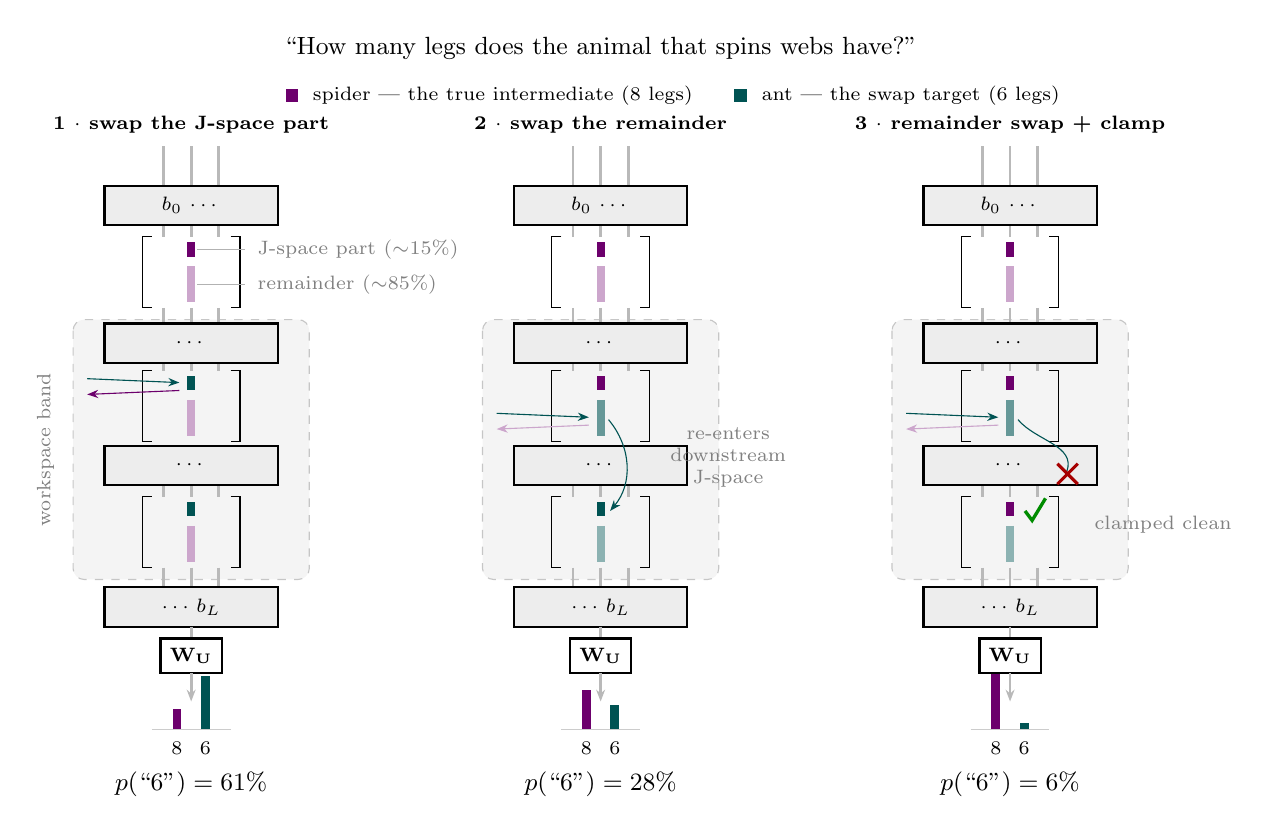
\begin{tikzpicture}
% ---- the prompt, once, at the top
\node[jlab] at (5.2,1.6) {``How many legs does the animal that spins webs have?''};
\fill[jvio] (1.2,0.92) rectangle +(0.16,0.16);
\node[jlabS,right] at (1.42,1.0) {spider --- the true intermediate (8 legs)};
\fill[jtea] (6.9,0.92) rectangle +(0.16,0.16);
\node[jlabS,right] at (7.12,1.0) {ant --- the swap target (6 legs)};
% ---- three panels: the common stack, then per-prong content
\foreach \PX in {0,5.2,10.4}{
\begin{scope}[xshift=\PX cm]
  % the workspace band, behind everything
  \fill[gray!9,rounded corners=4pt] (-1.5,-1.85) rectangle (1.5,-5.15);
  \draw[gray!45,dashed,rounded corners=4pt] (-1.5,-1.85) rectangle (1.5,-5.15);
  % cords (all token positions, bundled)
  \foreach \X in {-0.35,0,0.35}{
    \draw[cordJ] (\X,0.35) -- (\X,-0.15);
    \draw[cordJ] (\X,-0.65) -- (\X,-0.8);
    \draw[cordJ] (\X,-1.7) -- (\X,-1.9);
    \draw[cordJ] (\X,-2.4) -- (\X,-2.5);
    \draw[cordJ] (\X,-3.95) -- (\X,-4.1);
    \draw[cordJ] (\X,-5.0) -- (\X,-5.25);}
  % blocks
  \node[jband] at (0,-0.4) {$b_0\,\cdots$};
  \node[jband] at (0,-2.15) {$\cdots$};
  \node[jband] at (0,-3.7) {$\cdots$};
  \node[jband] at (0,-5.5) {$\cdots\,b_L$};
  \draw[cordJ] (0,-5.75) -- (0,-5.9);
  \node[draw,thick,font=\scriptsize] at (0,-6.12) {$\mathbf{W_U}$};
  \draw[cordJ,-{Stealth[length=1.5mm]}] (0,-6.34) -- (0,-6.7);
  % outcome axis + token labels
  \draw[gray!40] (-0.5,-7.05) -- (0.5,-7.05);
  \node[jlabS] at (-0.18,-7.3) {8};
  \node[jlabS] at (0.18,-7.3) {6};
\end{scope}}
% ---- panel 1: swap the J-space part
\begin{scope}
  \node[jlabS] at (0,0.62) {\textbf{1 $\cdot$ swap the J-space part}};
  \jglyph{-1.25}{jvio}{jvio!35}
  \jglyph{-2.95}{jtea}{jvio!35}
  \jglyph{-4.55}{jtea}{jvio!35}
  \draw[jtea,-{Stealth[length=1.4mm]}] (-1.32,-2.6) -- (-0.15,-2.65);
  \draw[jvio,-{Stealth[length=1.4mm]}] (-0.15,-2.75) -- (-1.32,-2.8);
  % anatomy labels, once
  \node[jlabS,gray,right] at (0.72,-0.96) {J-space part ($\sim$15\%)};
  \draw[gray!60,thin] (0.68,-0.96) -- (0.08,-0.96);
  \node[jlabS,gray,right] at (0.72,-1.4) {remainder ($\sim$85\%)};
  \draw[gray!60,thin] (0.68,-1.4) -- (0.08,-1.4);
  % band label
  \node[jlabS,gray,rotate=90] at (-1.85,-3.5) {workspace band};
  % outcome
  \draw[jvio,line width=3.2pt] (-0.18,-7.05) -- ++(0,0.26);
  \draw[jtea,line width=3.2pt] (0.18,-7.05) -- ++(0,0.67);
  \node[jlab] at (0,-7.75) {$p(\text{``6''}) = 61\%$};
\end{scope}
% ---- panel 2: swap the remainder; it re-enters downstream J-space
\begin{scope}[xshift=5.2cm]
  \node[jlabS] at (0,0.62) {\textbf{2 $\cdot$ swap the remainder}};
  \jglyph{-1.25}{jvio}{jvio!35}
  \jglyph{-2.95}{jvio}{jtea!60}
  \jglyph{-4.55}{jtea}{jtea!45}
  \draw[jtea,-{Stealth[length=1.4mm]}] (-1.32,-3.04) -- (-0.15,-3.09);
  \draw[jvio!35,-{Stealth[length=1.4mm]}] (-0.15,-3.19) -- (-1.32,-3.24);
  \draw[jtea,thin,-{Stealth[length=1.4mm]}] (0.1,-3.12) to[out=-50,in=50] (0.12,-4.28);
  \node[jlabS,gray,align=center] at (1.62,-3.6) {re-enters\\downstream\\J-space};
  \draw[jvio,line width=3.2pt] (-0.18,-7.05) -- ++(0,0.5);
  \draw[jtea,line width=3.2pt] (0.18,-7.05) -- ++(0,0.31);
  \node[jlab] at (0,-7.75) {$p(\text{``6''}) = 28\%$};
\end{scope}
% ---- panel 3: remainder swap + clamp the downstream J-space
\begin{scope}[xshift=10.4cm]
  \node[jlabS] at (0,0.62) {\textbf{3 $\cdot$ remainder swap + clamp}};
  \jglyph{-1.25}{jvio}{jvio!35}
  \jglyph{-2.95}{jvio}{jtea!60}
  \jglyph{-4.55}{jvio}{jtea!45}
  \draw[jtea,-{Stealth[length=1.4mm]}] (-1.32,-3.04) -- (-0.15,-3.09);
  \draw[jvio!35,-{Stealth[length=1.4mm]}] (-0.15,-3.19) -- (-1.32,-3.24);
  \draw[jtea,thin] (0.1,-3.12) to[out=-50,in=70] (0.72,-3.78);
  \draw[jdn,line width=1.1pt] (0.6,-3.68) -- (0.86,-3.94);
  \draw[jdn,line width=1.1pt] (0.6,-3.94) -- (0.86,-3.68);
  \draw[jgrn,line width=1.2pt] (0.19,-4.28) -- (0.28,-4.4) -- (0.45,-4.12);
  \node[jlabS,gray,right] at (0.95,-4.45) {clamped clean};
  \draw[jvio,line width=3.2pt] (-0.18,-7.05) -- ++(0,0.7);
  \draw[jtea,line width=3.2pt] (0.18,-7.05) -- ++(0,0.08);
  \node[jlab] at (0,-7.75) {$p(\text{``6''}) = 6\%$};
\end{scope}
\end{tikzpicture}}
\caption{The three-pronged swap. The probe direction for the unspoken intermediate (spider) splits into a J-space part---a sparse nonnegative combination of $k{=}25$ lens rows, only ${\sim}15\%$ of the probe's variance---and the ${\sim}85\%$ remainder. All interventions act at every layer of the workspace band, at every token position. \textbf{(1)} Swapping just the J-space part for ant's flips the answer $61\%$ of the time. \textbf{(2)} Swapping only the remainder still works $28\%$ of the time---but only because downstream layers read the moved content and re-express it into their own J-space (teal arrow). \textbf{(3)} Same remainder swap with the downstream J-space coordinates clamped to their clean (spider) values: the re-entry is blocked and the effect collapses to $6\%$. The ${\sim}15\%$ carries the causal freight; the ${\sim}85\%$ moves behavior only by being re-admitted into J-space.}
\label{fig:three-prong}
\end{figure}




\subsection{Further Questions Askable}
Tracing dispositional alignment as abstraction, tracing robustness of dispositional abstraction.


% ============================================================================
% RELOCATED FROM THE INTRO (this was the lofty opening of Section 1). Moved
% here at Ben's request so the paper opens practical/intuitive and closes on
% this crystallizing reflection.
% TODO (Ben):
%   - Title this section (candidates: 'Causal Privilege' / 'Legible Cause' /
%     'The Privilege We Beckoned'). Placeholder below --- rename.
%   - Dedupe against the whistling coda that follows AND your standalone
%     cause/privilege draft --- all three overlap.
%   - Decide whether this or 'J-vision, Generally' should be the true finale
%     (this currently precedes it; swap if you want it last).
% ============================================================================
\section{Causal Privilege}

Calculus is the language of cause. To influence a system purposefully, to understand it to the point of intervention, one must map its elements for their causal privilege.

Through the Jacobian Lens (\textbf{J-lens}), Anthropic has \href{https://transformer-circuits.pub/2026/workspace/index.html}{found} the \textbf{J-space}: a causally privileged set of levers that training discovered, bootstrapped, and put to use. Through it, we begin to wrest the most vexing curse of deep learning. Ceding the manual construction of a hierarchy of causal privilege, we let backpropagation---whose perceptual field and logic of influence is calculus---deliver us a coherent system to the understanding of whose logic we held no initial claim. Stunning proficiency outran stable understanding. That we've now found this leverage and made it legible in a system that draws such due awe is an achievement to behold---and to excite.

The \textbf{J-space} is not an end reached, but the first revelation of the internal coherence we let emerge. Endowed with too much representational and algorithmic capacity, these systems crystallized an obvious coherence. For such a jungle to behave so coherently, there had to have been hierarchies formed, the effective complexity had to have collapsed, local tendencies had to be bent \textit{upward} in service of a productive coarse-graining. This is causal emergence.\footnote{\textit{Causal emergence} is a technical notion (Hoel, Albantakis, and Tononi, 2013): a coarse-grained \textit{macro}-scale of a system can hold \textit{more} causal power---a higher \textit{effective information}---than the fine-grained \textit{micro}-scale beneath it. It is invoked here deliberately rather than as loose metaphor: the model's behavior is steered by a few macro-directions that training distilled from a vastly over-parameterized micro-substrate---the very privilege that later sections render legible and manipulable.} What better equipment with which to re-discover the causal structures we've coerced to emerge than the language of cause itself?

% EXPAND (Ben, prose): the 'organized hierarchically ... success without' sentence and 'reflected our choice domain' below are the crux but dense --- worth unpacking (within/without = internal structure vs external competence; 'choice domain' = the domain we chose to situate the model in).
Coloring the network with legible causal links is an old achievement. Only when the models proved to have organized hierarchically, to have allocated privilege non-uniformly within as evidenced by the non-trivial success without, was it time to peel the layers back and find that privilege. Random networks can be interpreted end-to-end in terms of legible cause. Only when they evidenced to have reflected our choice domain into their internal mechanism did we have---at once---the ability and obligation to find that reflection in the form of privileged neural circuits.


% ============================================================================
% SEED (Ben --- for the Causal Privilege thesis; prose is yours). PERSUADABILITY.
%
% Ben's core: causal privilege is deeply tied to PERSUADABILITY (Michael Levin's
% sense). It relates to causal emergence and to low entropy. The point --- you can
% intervene on and steer the system very THINLY and very far UPSTREAM, and here
% very LEGIBLY (the swaps), without micromanaging weights or mechanism. The system
% is one of NESTED COMPETENCY: stable enough to interpret a high-level change and
% land on its feet. The key quantity is a leverage ratio, SizeOfActionCaused /
% SizeOfPrompt (where 'size' is doing heavy, ambiguous work). Human beings are
% amazing because one spark in the tiny neurons of a small brain can, by thinly
% intervening on other humans, move mountains. You need no biology to get your dog
% to sit; no muscle fibers or chemistry to get yourself out of bed and make the
% coffee you WANT. J-space is showing itself as one of these highly-levered
% persuadability protocols --- one that, I think, both we AND the model itself
% have independently discovered.
%
% CONNECTIONS to lean on:
%   - Levin (TAME / 'agential materials'): you address a competent system at the
%     level it can be *convinced*, not rewired --- e.g. bioelectric goal-signals
%     reprogram morphology without editing the genome. Same shape: high-level
%     setpoint in, coherent low-level reorganization out, hardware left untouched.
%   - Causal emergence (the S6 footnote): the lever lives on a coarse-grained
%     MACRO variable --- which is exactly why a thin macro-nudge has coherent reach.
%   - Low entropy: the control manifold is tiny (a few dozen directions) next to
%     the full state --- a compressed, low-entropy channel INTO the system.
%   - The swaps (three-prong figure): the empirical anchor --- ~15% of the probe's
%     variance carries ~60% of the behavior. Leverage, measured.
%   - The whistling section (S7) already carries the sibling idea: high-level goals
%     filtering down through nested mechanism; fibers; 'executive steering'.
%     Persuadability is that family --- decide whether it lives here, there, or
%     bridges the two (standing risk: three overlapping codas).
%
% WARNINGS / to sharpen before it becomes prose:
%   - The ratio ALONE is not the concept. Chaos also has huge effect/cause ratios
%     (the butterfly) yet is neither steerable nor legible. Persuadability =
%     leverage + PREDICTABILITY + the system's self-stabilizing competence to
%     absorb the nudge and land on its feet. Say this or a reader will conflate
%     leverage with mere sensitivity.
%   - Define 'size'. Bits? Description length? Dimensionality? Norm? It is load-
%     bearing --- pick a reading (I'd lean description-length / dimensionality of
%     the intervention vs. the coherent scope of the downstream change) and name it.
%   - 'Both we and the model independently discovered it' is a strong, lovely claim
%     --- ground it in the finding that downstream weights AMPLIFY J-space
%     directions (the model built its own high-leverage control surface; we merely
%     learned to read and push it). Mirrors S7's 'internal apprehension of high-
%     leverage states'.
%   - Levin is a specific researcher with specific empirical claims (bioelectricity,
%     regeneration). Frame as resonance/analogy, not equivalence; cite him as such
%     and don't imply he said anything about LLMs.
% ============================================================================
\section{The Horizons of J-vision}

As I wrote this document, I stepped out to pick up dinner and indulged in a whistle-along car ride. I am a good whistler, but tonight there was unusual accord between the sounds I wanted and those that were broadcast from my mouth. It stirred me to think about the control my brain was exerting over many distinct modules of my body. The physics of human whistling are far beyond my competency, and I know for sure its theorems and equations are etched nowhere in my brain. All that my brain needs to know to realize my conviction---which we won't bother interrogating today---is a \textbf{J-lens} differentiating \textit{whistled frequency} with respect to what I am loosely imagining as a stream of \textit{electrical command vectors} propagating from my brain to my diaphragm, lungs, throat, lips, and tongue. The algorithm does not need realization, only \(\mathbb{E} [\frac {\partial \mathbf{Pitch}}  {\partial \mathbf{Command}}]\) does (and even this quantity is not \textit{realized}, but baked into the machinery).

Why \(\mathbb{E}\)? I can whistle with similar aptitude across many different physical contexts; wet lips after a shower, dry lips on a cold winter day, laying on my back, walking on the treadmill, engaging my tongue or not, optimizing for volume or exactness...In each context, the machine to control is slightly different, but the function that describes how to change notes in any of these contexts is overwhelmingly quite similar. Whatever the realization of the whistling \textbf{J-lens} in my brain, it is an average over contexts. I can pick up whistling without having any conscious awareness of the moisture on my lips or in the air. Sure, once this information is known, there's some steering and tuning that occurs (the \textbf{J-lens} is not all-seeing, the \textbf{J-space} does not exist or act alone!), but there is a directional map of where to go in \textit{electrical command space} to reach a desired location in \textit{whistled frequency space}. 

One more feature of the whistling lens bears mentioning here, as it relates to robustness of disposition. The map from \textit{command space} to \textit{frequency space} is \textit{non-injective,} meaning it exhibits \textbf{many-to-one} relationships. There are many, many specific commands my brain can stream that will achieve the same frequency, especially when the diverse contexts above are considered. There is, then, a notion of \textit{fibers} with respect to this map. There are directions in command space that can be traversed that will not change the corresponding output in frequency space. If I want to stay on tune and remain alive, I must breathe through my performance; my brain evidently has found invariant fibers along which it should travel in command space as the periods of respiration occur. The same idea goes for the moisture of my lips, which is constantly changing, especially when I whistle. There are circuits in the brain that can pin the required invariant---pitch---with a proficient honoring of the fibers admitted under the \textbf{J-lens}. \textbf{J-vision} gives us a new intuitive vocabulary with which to explain cybernetics---in differentiable and non-differentiable machines alike. 

The mystery of how high-level mental goals filter down through mechanism into realization has always tantalized me. \textbf{J-vision} is the beginning of the answer. Anthropic's results suggested that Claude's downstream weights specifically amplify privileged \textbf{J-space} directions internally, and we have to imagine that such a privileged space (in any layer \(\ell\)) developed in concert with other parameters (in layers \(\ell' < \ell\)) that learned to exert high-leverage influence on the future behavior of the model by manifesting changes in  \(h_\ell\). But beyond a system's internal apprehension (by way of \textbf{J-vision}) of its high leverage states, we as machine learning engineers are tantalized by \textit{our own} interventional opportunities as \textit{external} agents. If the brain has modules akin to language models, we can imagine that higher-level systems have found their own levered hooks informed by \textbf{J-vision} as well that can enable executive steering. 

\textbf{J-vision} is both the generalized ability to map changes in high-leverage control variables to those in downstream domains of behavior \textit{as well as} the disposition to think about and look at hierarchical systems in this framing. \textbf{J-vision} seeks \textbf{J-vision}. We've just gotten our first \textbf{J-glimpse}. 

\end{document}

